\documentclass{cmspaper}
\usepackage{graphicx}
\usepackage{amsmath}
\usepackage{amssymb}
\usepackage{subfigure}
\usepackage{multirow}
\usepackage[pdfborder=0 0 0,
            colorlinks,
            urlcolor = blue,
            linkcolor = black,
            citecolor = black,
            menucolor = black,]
           {hyperref}
%% \usepackage[colorlinks]{hyperref}
%% \usepackage{url}
\usepackage[toc,page]{appendix}
\usepackage{varioref} 
\renewcommand{\appendixname}{Appendix}
%% \renewcommand{\appendixtocname}{List of appendices}

% % useful definitions

% processes
\def\dyee {\ensuremath{Z/\gamma^*\to ee}}
\def\dymm {\ensuremath{Z/\gamma^*\to\mu\mu}}
\def\dytt {\ensuremath{Z/\gamma^*\to\tau\tau}}
\def\zee {\ensuremath{Z\to ee}}
\def\zmm {\ensuremath{Z\to\mu\mu}}
\def\ztt {\ensuremath{Z\to\tau\tau}}
\def\ttbar {\ensuremath{t\bar{t}}}
\def\wwll {\ensuremath{WW\to l^+l^-}}
\def\wwlulu{\ensuremath{WW\to l^+\nu l^-\bar{\nu}}}
\def\ww {\ensuremath{WW}}
\def\hww {\ensuremath{H\to WW}}
\def\wz{\ensuremath{WZ}}
\def\zz{\ensuremath{ZZ}}
\def\wgamma{\ensuremath{W\gamma}}
\def\wjets{\ensuremath{W+}jets} 
\def\tw{\ensuremath{tW}} 
\def\singletopt{\ensuremath{t} ($t$-chan)} 
\def\singletops{\ensuremath{t} ($s$-chan)} 
\def\all{all}
\def\ee{\ensuremath{ee}}
\def\emu{\ensuremath{e\mu}}
\def\mm{\ensuremath{\mu\mu}}

%units
\newcommand{\TeV}{\ensuremath{\mathrm{Te\kern -0.1em V}}}
\newcommand{\GeV}{\ensuremath{\mathrm{Ge\kern -0.1em V}}}

%others
\def\pt{\ensuremath{p_T}}
\def\ipb{pb\ensuremath{^{-1}}}
\def\ifb{fb\ensuremath{^{-1}}}
\def\et{\ensuremath{E_T}}
\def\met{\ensuremath{E\!\!\!\!/_T}}
\def\fBrem{\ensuremath{f_{\rm brem}}}
\def\pin{\ensuremath{p_{\rm in}}}
\def\pout{\ensuremath{p_{\rm out}}}

\newcommand{\CLs}{\ensuremath{CL_\mathrm{s}}}
\newcommand{\CLb}{\ensuremath{CL_\mathrm{b}}}
\newcommand{\CLsb}{\ensuremath{CL_\mathrm{s+b}}}

\newcommand{\GeV}{\ensuremath{\mathrm{Ge\kern -0.1em V}}}
\newcommand{\TeV}{\ensuremath{\mathrm{Te\kern -0.1em V}}}
\newcommand{\TeVcc}{\ensuremath{\,\mathrm{Te\kern -0.1em V\!/c}^2}}
\newcommand{\GeVcc}{\ensuremath{\,\mathrm{Ge\kern -0.1em V\!/c}^2}}
\newcommand{\MeVcc}{\ensuremath{\,\mathrm{Me\kern -0.1em V\!/c}^2}}
\newcommand{\GeVc}{\ensuremath{\mathrm{Ge\kern -0.1em V}\!/c}}
\newcommand{\nanob}{\mbox{{\rm ~nb}~}}
\newcommand{\fb}{\ensuremath{\mathrm{fb}}}
\newcommand{\pb}{\ensuremath{\mathrm{pb}}}
\newcommand{\ifb}{\ensuremath{\mathrm{fb^{-1}}}}
\newcommand{\ipb}{\ensuremath{\mathrm{pb^{-1}}}}
\newcommand{\grad}{\ensuremath{^{\circ}}}
%
% Special user made math symbols
%
\newcommand{\lsim}{\raisebox{-1.5mm}{$\:\stackrel{\textstyle{<}}{\textstyle{\sim}}\:$}}
\newcommand{\gsim}{\raisebox{-1.5mm}{$\:\stackrel{\textstyle{>}}{\textstyle{\sim}}\:$}}

% particles

\newcommand{\pipm}{\ensuremath{\pi^{\pm}}}
\newcommand{\pizero}{\ensuremath{\pi^{0}}}
\newcommand{\Hi}{\ensuremath{\mathrm{H}}}
\newcommand{\W}{\ensuremath{\mathrm{W}}}
\newcommand{\Wjets}{\ensuremath{\mathrm{W+jets}}}
\newcommand{\Zjets}{\ensuremath{\mathrm{Z+jets}}}
\newcommand{\Wt}{\ensuremath{\mathrm{Wt}}}
\newcommand{\Wstar}{\ensuremath{\mathrm{W}^{*}}}
\newcommand{\Wparenthesisstar}{\ensuremath{\mathrm{W}^{(*)}}}
\newcommand{\WW}{\ensuremath{\W^+\W^-}}
\newcommand{\Z}{\ensuremath{\mathrm{Z}}}
\newcommand{\Zstar}{\ensuremath{\mathrm{Z}^{*}}}
\newcommand{\Astar}{\ensuremath{\mathrm{\gamma}^{*}}}
\newcommand{\ZZ}{\ensuremath{\Z\Z}}
\newcommand{\WZ}{\ensuremath{\W\Z}}
\newcommand{\Wgstar}{\ensuremath{\W\Astar}}
\newcommand{\E}{\ensuremath{\mathrm{e}}}
\newcommand{\Ep}{\ensuremath{\mathrm{e}^{+}}}
\newcommand{\Em}{\ensuremath{\mathrm{e}^{-}}}
\newcommand{\Epm}{\ensuremath{\mathrm{e}^{\pm}}}
\newcommand{\Emp}{\ensuremath{\mathrm{e}^{\mp}}}
\newcommand{\M}{\ensuremath{\mu}}
\newcommand{\Mp}{\ensuremath{\mu^{+}}}
\newcommand{\Mm}{\ensuremath{\mu^{-}}}
\newcommand{\Mpm}{\ensuremath{\mu^{\pm}}}
\newcommand{\Mmp}{\ensuremath{\mu^{\mp}}}
\newcommand{\Tau}{\ensuremath{\tau}}
\newcommand{\Nu}{\ensuremath{\nu}}
\newcommand{\Nubar}{\ensuremath{\bar{\nu}}}
\newcommand{\Lep}{\ensuremath{\ell}}
\newcommand{\Lepp}{\ensuremath{\ell^{+}}}
\newcommand{\Lepm}{\ensuremath{\ell^{-}}}
\newcommand{\Lprime}{\ensuremath{\Lep^{\prime}}}
\newcommand{\Prot}{\ensuremath{\mathrm{p}}}
\newcommand{\Pbar}{\ensuremath{\bar{\mathrm{p}}}}
\newcommand{\PP}{\Prot\Prot}
\newcommand{\PPbar}{\Prot\Pbar}
\newcommand{\ttbar}{\ensuremath{\mathrm{t}\bar{\mathrm{t}}}}
\newcommand{\qq}{\ensuremath{\mathrm{q}\mathrm{q}}}
%\newcommand{\bbbar}{\ensuremath{\mathrm{b}\bar{\mathrm{b}}}}
\newcommand{\Wtb}{\ensuremath{\W\mathrm{t}\mathrm{b}}}
\newcommand{\Top}{\ensuremath{\mathrm{t}}}
\newcommand{\Bot}{\ensuremath{\mathrm{b}}}
\newcommand{\Atop}{\ensuremath{\bar{\mathrm{t}}}}
\newcommand{\Abot}{\ensuremath{\bar{\mathrm{b}}}}
% arrow
\newcommand{\To}{\ensuremath{\rightarrow}}

% masses
\newcommand{\mHi}{\ensuremath{m_{\mathrm{H}}}}
\newcommand{\mW}{\ensuremath{m_{\mathrm{W}}}}
\newcommand{\mZ}{\ensuremath{m_{\mathrm{Z}}}}
\newcommand{\mll}{\ensuremath{m_{\Lep\Lep}}}
\newcommand{\mt}{\ensuremath{m_{\mathrm{T}}}}

% kinematics
\newcommand{\pt}{\ensuremath{p_\mathrm{T}}}
\newcommand{\ptveto}{\ensuremath{\pt^\mathrm{veto}}}
\newcommand{\ptl}{\ensuremath{p_\perp^{\Lep}}}
\newcommand{\ptlmax}{\ensuremath{p_{\mathrm{T}}^{\Lep,\mathrm{max}}}}
\newcommand{\ptlmin}{\ensuremath{p_{\mathrm{T}}^{\Lep,\mathrm{min}}}}
\newcommand{\met}{\ensuremath{\Et^{\mathrm{miss}}}}
\newcommand{\delphill}{\ensuremath{\Delta\phi_{\Lep\Lep}}}
\newcommand{\deletall}{\ensuremath{\Delta\eta_{\Lep\Lep}}}
\newcommand{\delphimetl}{\ensuremath{\Delta\phi_{\met\Lep}}}
\newcommand{\Et}{\ensuremath{E_\mathrm{T}}}
\newcommand{\delR}{\ensuremath{\Delta R}}
\newcommand{\Eta}{\ensuremath{\eta}}

%efficiencies
\newcommand{\effsig}{\ensuremath{\varepsilon_{\mathrm{bkg}}^{\mathrm{S}}}}
\newcommand{\effnorm}{\ensuremath{\varepsilon_{\mathrm{bkg}}^{\mathrm{N}}}}
\newcommand{\Nsig}{\ensuremath{N_{\mathrm{bkg}}^{\mathrm{S}}}}
\newcommand{\Nnorm}{\ensuremath{N_{\mathrm{bkg}}^{\mathrm{N}}}}

% processes
\newcommand{\dyee}{\ensuremath{Z/\gamma^*\to ee}}
\newcommand{\dymm}{\ensuremath{Z/\gamma^*\to\mu\mu}}
\newcommand{\dytt}{\ensuremath{Z/\gamma^*\to\tau\tau}}
\newcommand{\dyll}{\ensuremath{Z/\gamma^*\to\ell\ell}}
\newcommand{\dy}{\ensuremath{Z/\gamma^*}}
\newcommand{\zee}{\ensuremath{Z\to ee}}
\newcommand{\zmm}{\ensuremath{Z\to\mu\mu}}
\newcommand{\ztt}{\ensuremath{Z\to\tau\tau}}
%\newcommand{\ttbar}{\ensuremath{t\bar{t}}}
\newcommand{\ppww}{\ensuremath{pp \to W^+W^-}}
\newcommand{\wwll}{\ensuremath{WW\to \ell^+\ell^-}}
\newcommand{\wwlnln}{\ensuremath{W^+W^-\to \ell^+\nu \ell^-\bar{\nu}}}
\newcommand{\ww}{\ensuremath{WW}}
\newcommand{\wwpm}{\ensuremath{W^+W^-}}
\newcommand{\hww}{\ensuremath{H\to W^+W^-}}
\newcommand{\wz}{\ensuremath{WZ}}
\newcommand{\zz}{\ensuremath{ZZ}}
\newcommand{\wgamma}{\ensuremath{W\gamma}}
\newcommand{\wjets}{\ensuremath{W+}jets} 
\newcommand{\tw}{\ensuremath{tW}} 
\newcommand{\singletopt}{\ensuremath{t} ($t$-chan)} 
\newcommand{\singletops}{\ensuremath{t} ($s$-chan)} 
\newcommand{\zx}{\ensuremath{\mathrm{DY/WZ/ZZ}}}
\newcommand{\zv}{\ensuremath{\mathrm{WZ/ZZ}}}
\newcommand{\z}{\ensuremath{\mathrm{Z}}}
\newcommand{\routin}{\ensuremath{R_{out/in}}}

%other 
\def\fixme{({\bf FixMe})}
\newcommand{\ee}{\ensuremath{ee}}
\newcommand{\emu}{\ensuremath{e\mu}}
\def\mm{\ensuremath{\mu\mu}}

% integrated luminosity
\newcommand{\intlumiSevenTeV}{4.92~\ifb}
\newcommand{\intlumiEightTeV}{1.62~\ifb}

%%%%%%%%%%%
%
\newcounter{myfootertablecounter}

\newcommand\myfootnotemark{%
  %\refstepcounter{footnote}%
  \addtocounter{footnote}{1}%
  \footnotemark[\thefootnote]%
}%

\newcommand\myfootnotetext[1]{%
  \addtocounter{myfootertablecounter}{1}
  \footnotetext[\value{myfootertablecounter}]{#1}
}

% from now on, myfootnote has to be used rather than footnote to
% adapt the myfootercounter
\newcommand\myfootnote[1]{%
  \addtocounter{myfootertablecounter}{1}
  \footnote{#1}
}%



\setcounter{topnumber}{1}
\setcounter{bottomnumber}{1}
\setcounter{secnumdepth}{6}
%===================================================================================================
\begin{document}
\begin{titlepage}

  \analysisnote{2012/XXX}

  \date{\today}

  \title{A 2-dimensional Shape Analysis for Higgs Boson Search in the Fully Leptonic $W^+W^-$ Final State}

  \begin{Authlist}
%
L.~Bauerdick, K.~Burkett, I.~Fisk, Y.~Gao, O.~Gutsche, B.~Hooberman, S.~Jindariani, S.~Tkaczyk, V. Martinez Outschoorn, 
\Instfoot{fnal}{Fermilab National Accelerator Laboratory, Batavia, USA}
%
G.~Bauer, J.~Bendavid, E.~Butz, M.~Chan, V.~Dutta, G.~G\'omez-Ceballos, M.~Goncharov, K.~Hahn, P.~Harris, M.~Klute, S.~Nahn, C.~Paus, D.~Ralph, F.~Stoeckli, K.~Sumorok, K.~Sung, R.~Wolf, S.~Xie, M.~Yang, M.~Zanetti
\Instfoot{mit}{Laboratory for Nuclear Science, Massachusetts Institute of Technology, Cambridge, USA}
%
D.~Barge, C.~Campagnari, D.~Kovalskyi, V.~Krutelyov
\Instfoot{ucsb}{University of California, Santa Barbara, Santa Barbara, USA}
%
W.~Andrews, G.~Cerati, D.~Evans, F.~Golf, I.~MacNeill, S.~Padhi, Y.~Tu, F.~W\"urthwein, A.~Yagil, J.~Yoo
\Instfoot{ucsd}{University of California, San Diego, San Diego, USA}
%
I.~Kravchenko
\Instfoot{unl}{University of Nebraska-Lincoln, USA}

\end{Authlist}


  \begin{abstract}
    This note describes a 2-dimensional shape analysis searching
	for the Higgs boson in the $W^+W^- \to 2\ell2\nu$ final state. 
	The study is done with events in $e\mu$ final states containing 
	0 or 1 reconstructed jets. We report expected significances 
	in \intlumiEightTeV at $\sqrt s = 8~\TeV$ as well as projection
	to 20~\ifb.  
  \end{abstract} 

\end{titlepage}
\tableofcontents
%\listoftables
%\listoffigures
\newpage 

%===================================================================================================
\section{Introduction}
  \label{sec:overview}
  Precision measurement of the gauge boson couplings is a well known
method to look for physics beyond the Standard Model. In the case of
the triple gauge boson couplings, new physics contributions can be
expressed in the form of an effective Lagrangian. The most general
form of such a Lagrangian has 14 complex couplings (7 for $WWZ$ and 7 for
$WW\gamma$). Assuming electromagnetic gauge invariance, and C and P
symmetry conservation that number is reduced to five:
$\Delta\kappa_Z$, $\Delta g^Z_1$, $\Delta\kappa_{\gamma}$, $\lambda_Z$
and $\lambda_{\gamma}$. Applying gauge constraints:
\begin{align}
  \Delta\kappa_Z &= \Delta g^Z_1- \Delta\kappa_{\gamma}\tan^2\theta_W \\
  \lambda_Z &= \lambda_{\gamma}
\end{align}
further reduces the number of independent couplings to three. In the
Standard Model all five couplings are zero. 
 
CMS performed a first measurement of the anomalous couplings with
35/pb of data at 7 TeV~\cite{blah}. The measurement was performed with
and without a form factor that helps to avoid unitarity violation by
introducing an effective cutoff scale where a coupling is switched
off.  In this study we have two orders of magnitude more data and
experimental constraints on the couplings are more stringent then the
unitarity constraint. Therefore all the anomalous couplings are
form-factor free.

This analysis is based on the $W^+W^-$ production cross-section
measurement in $\intlumi$ of $pp$ collision data at $\sqrt{s} = $
7~$\TeV$ (the full 2011 dataset) \cite{ref:WWXS2011}. 

measurement~\cite{ref:WWXS2011}. Here we just briefly summarize the event
selection showing mostly kinematic requirements that may affect the
leading lepton pt distribution, which is used as a main observable.

The kinematic observable used in this analysis is 
the transverse momentum (\pt) of the leading lepton,
shown in Figure \ref{fig:pas_pt1_incl} after all event selections
have been applied.

\begin{figure}[hb]
\subfigure[Linear scale]{\label{subfig:pas_pt1_incl}
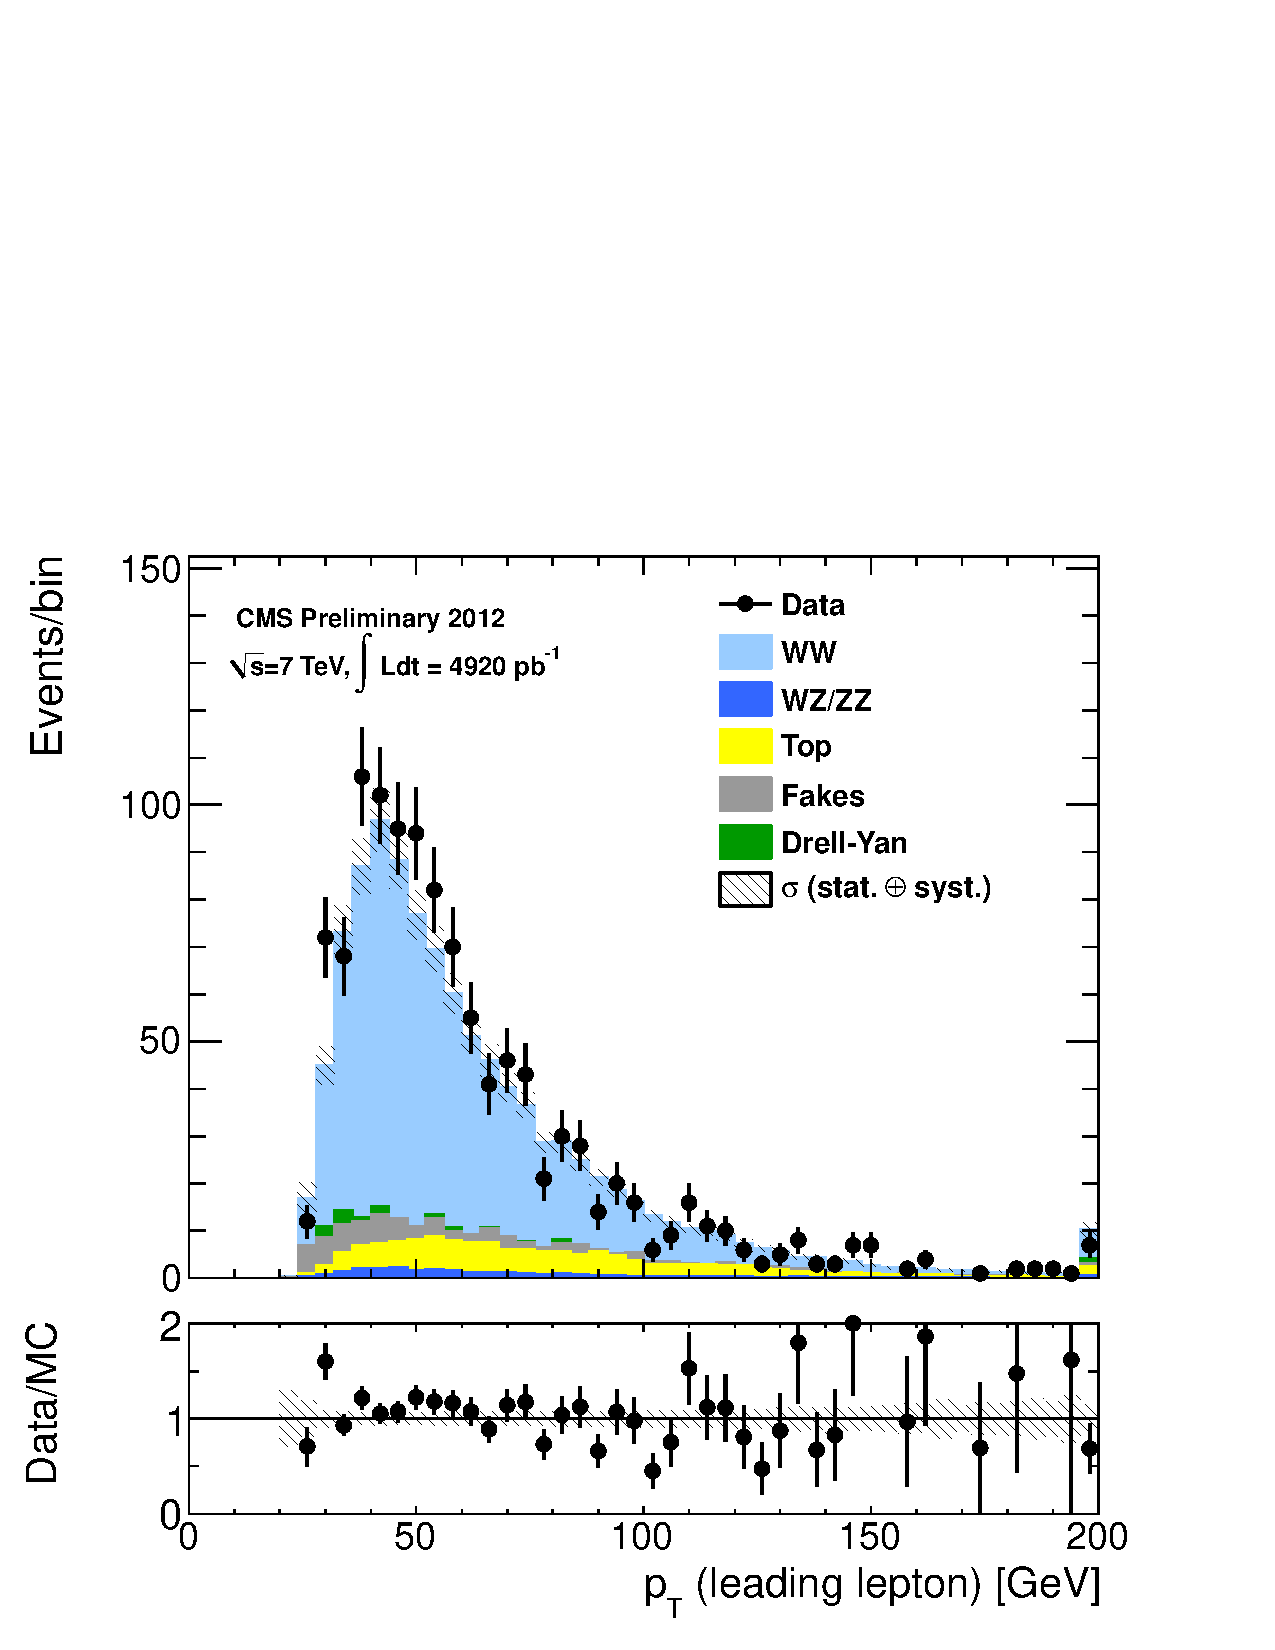
\includegraphics[width=.45\textwidth]{figures/pas_pt1_incl.pdf}}
\subfigure[Log scale]{\label{subfig:pas_pt1_incl_log}
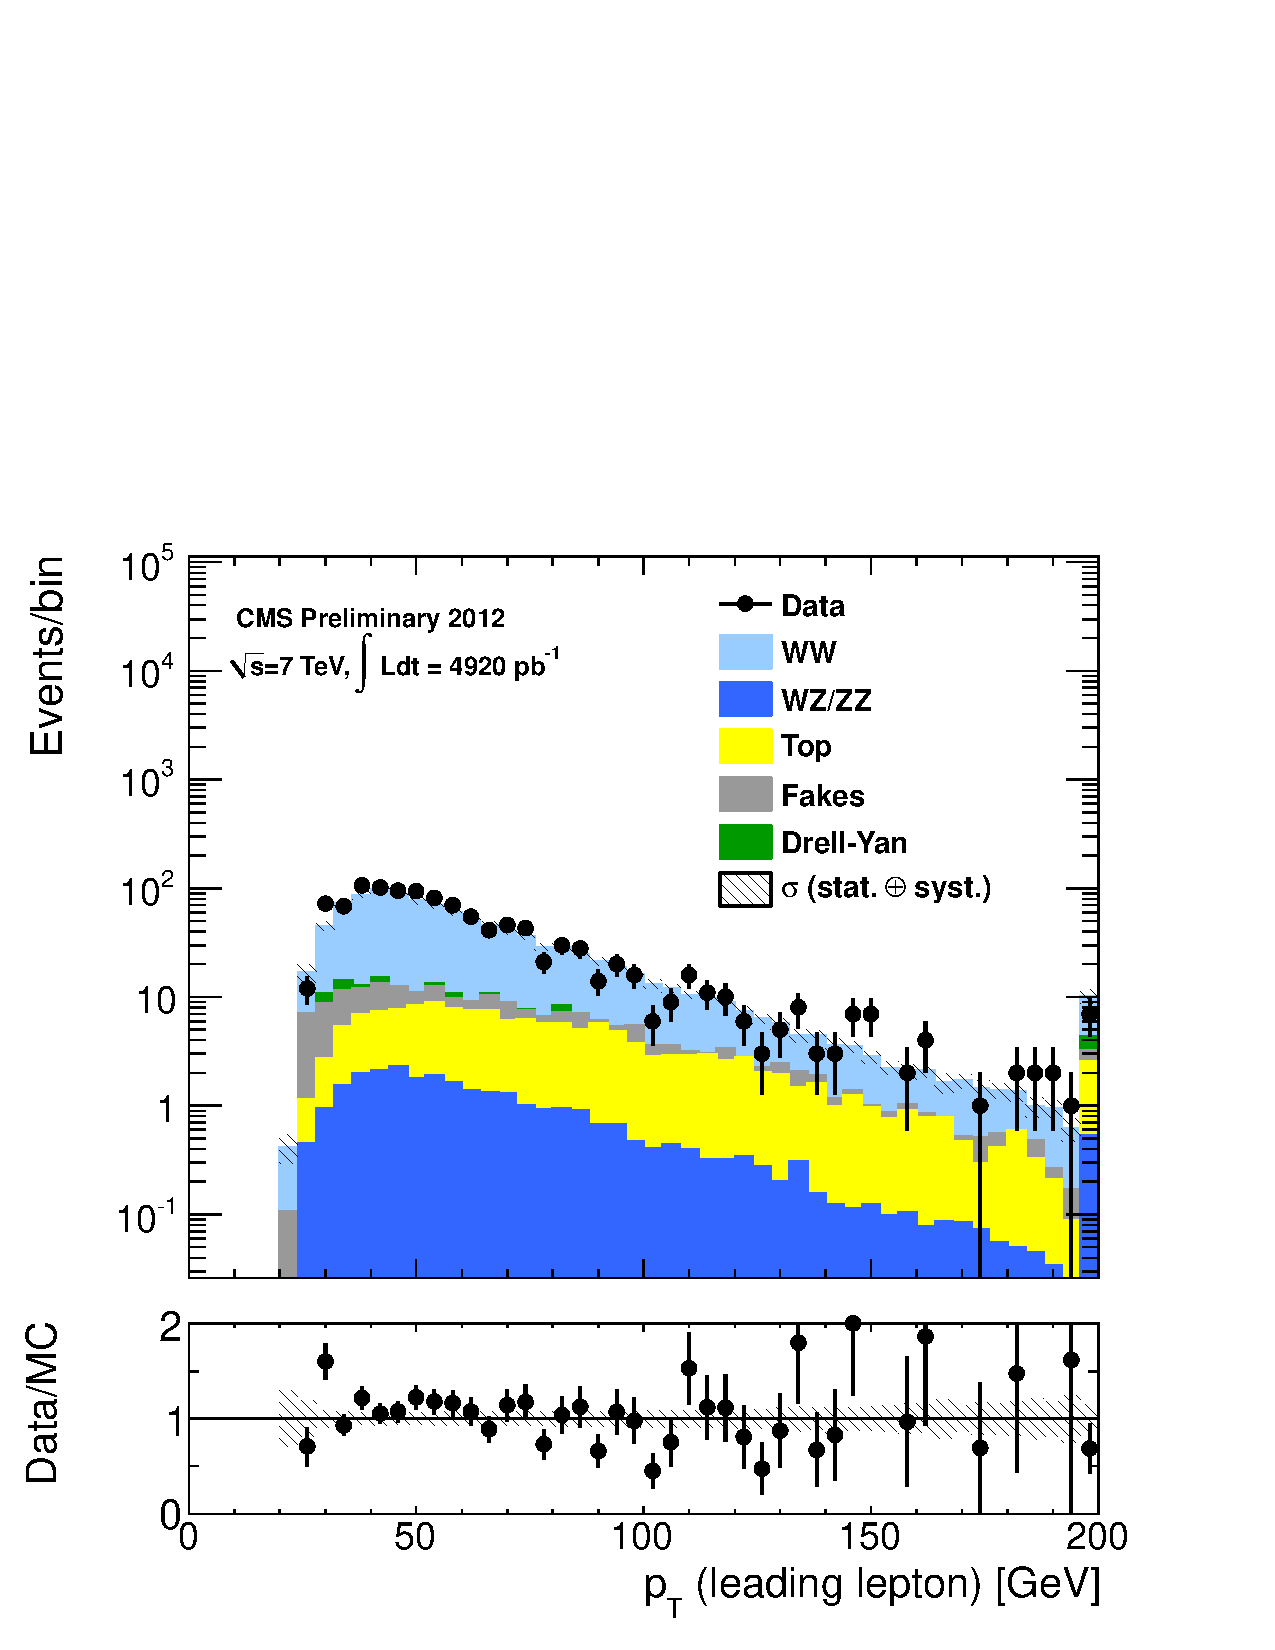
\includegraphics[width=.45\textwidth]{figures/pas_pt1_incl_log.pdf}}
\caption{Leading lepton \pt.}
\label{fig:pas_pt1_incl}
\end{figure}



%
\newpage
\section{Method}
  \label{sec:method}
  This section describes the details of the 2D method,
choice of variables, event selection, bin size, range, and 
unrolling technique. Then, follow 2D and unrolled templates
for signal and background processe. The last subsection 
describes shape uncertainties.


  \subsection{Choice of variables}
  \label{sec:choice_var}
  
The 2D templates are constructed using The \mll~and \mt~ variables.
These variables are defined as follows:

%
\begin{itemize}
\item the dilepton mass $\mll$;
\item transverse Higgs mass, 
$\mt^{\ell\ell\met} = \sqrt{2\pt^{ll}\met(1-cos(\Delta\phi_{\ell\ell-\met}))}$ where 
$\Delta\phi_{\ell\ell-\met}$ is the angle between dilepton
direction and \met in the transverse plane.
\end{itemize} 

Example templates are shown in 
Figure~\ref{fig:templates_125_ex} 
for the Higgs boson signal with a mass \mHi = 125 \GeV~(left) and 
the dominant \qqww~background (right). As expected, the 
\qqww~background peaks at higher values of \mll~than the signal.

%
\begin{figure}[!hbtp]
	
	%
	\centering
	\subfigure[Signal]{
	\centering
	\label{subfig:template_signal_125}
		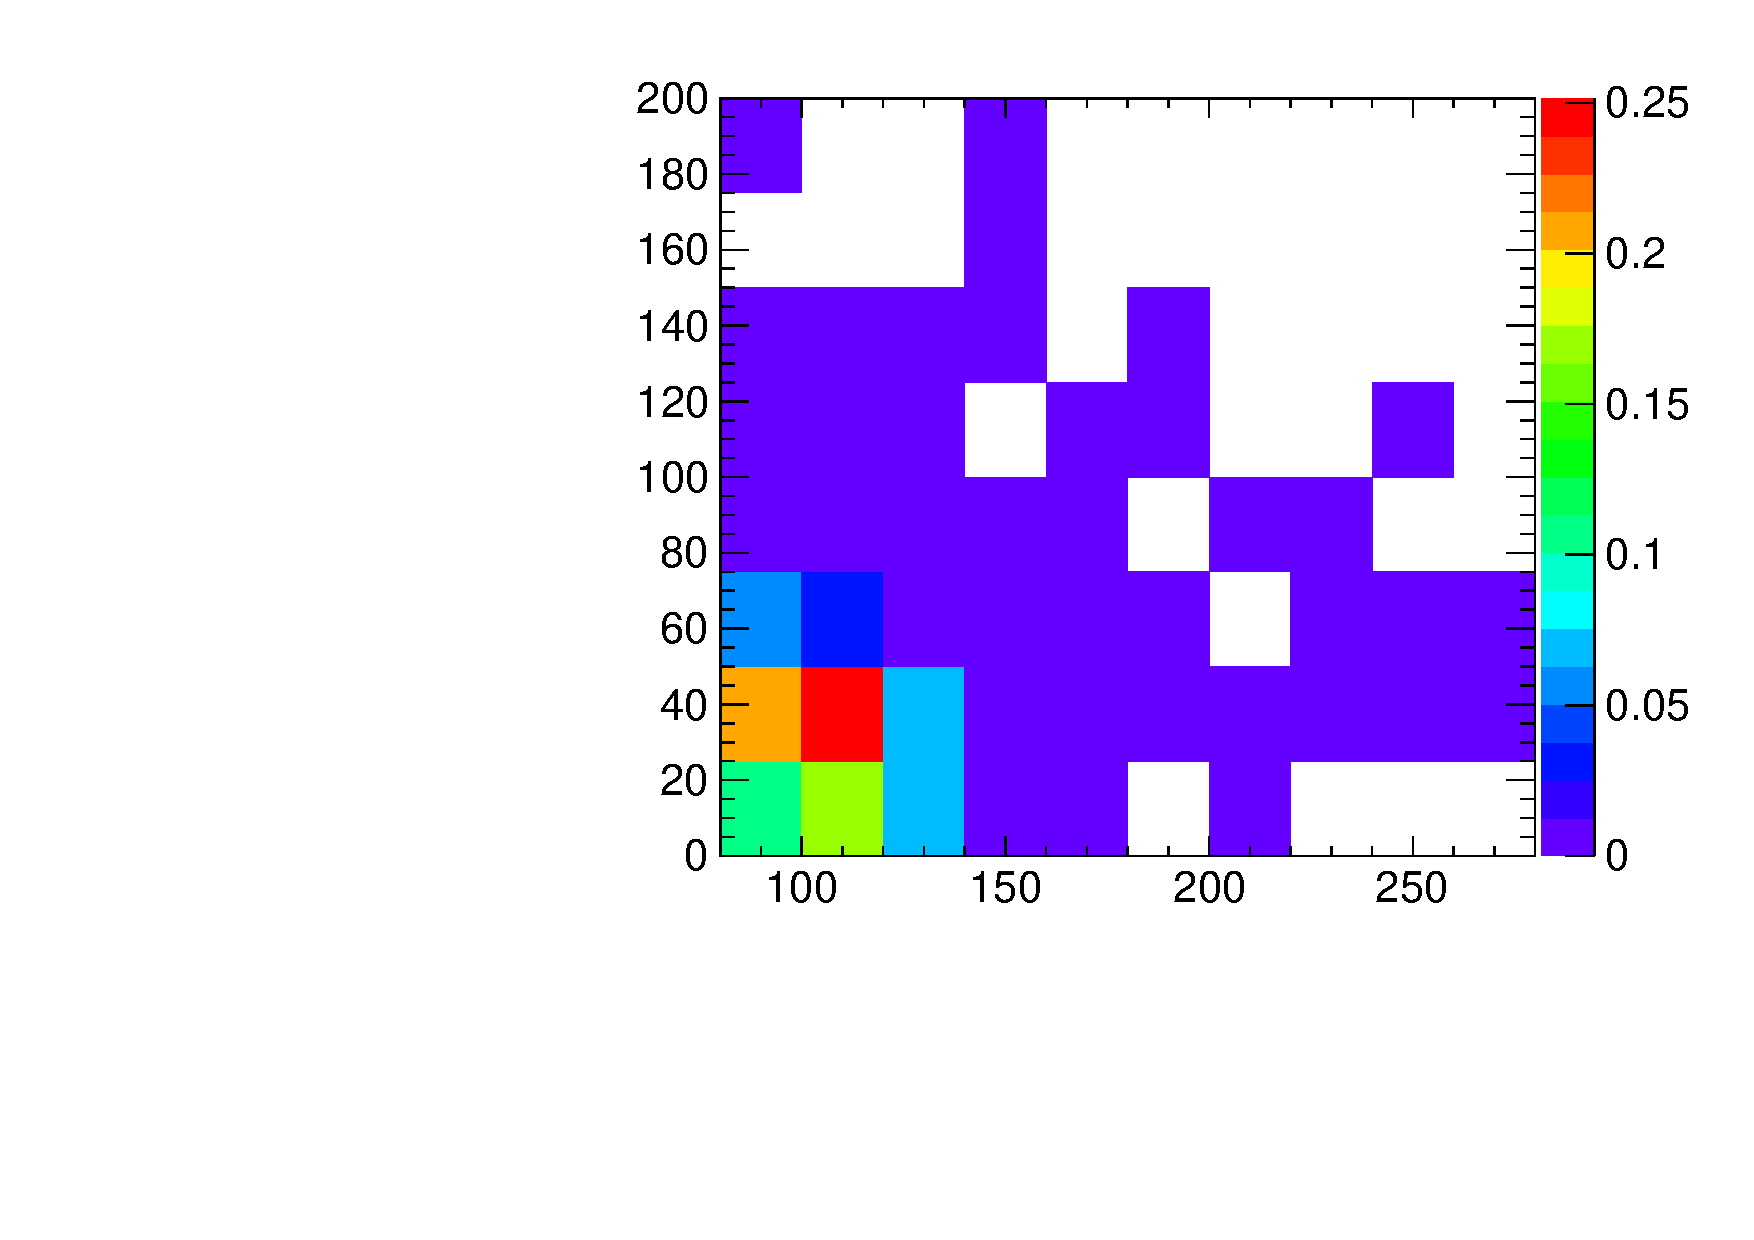
\includegraphics[width=.35\textwidth]{figures/templates/sig_2D_mH125_0j_of.pdf}
	}
	\subfigure[\qqww]{
	\centering
	\label{subfig:template_qqWW_125}
		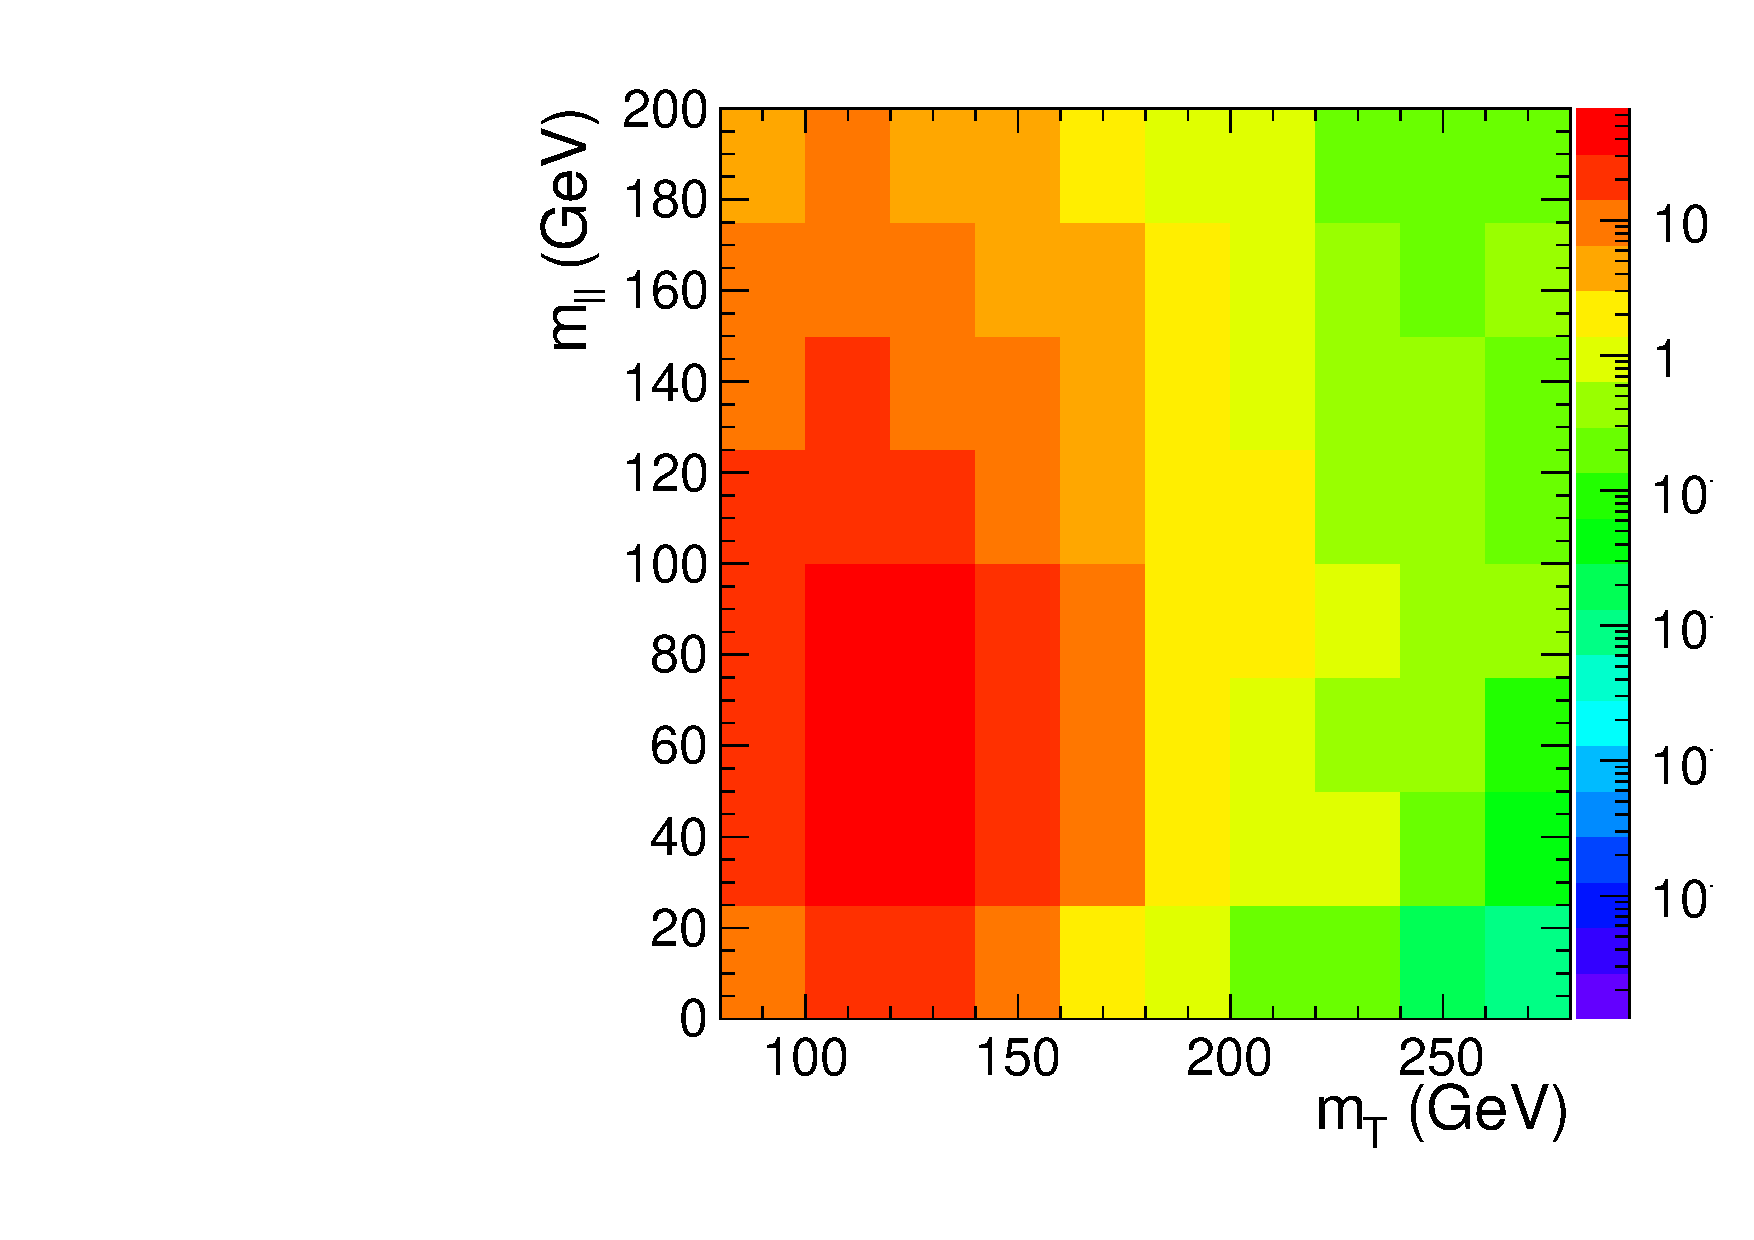
\includegraphics[width=.35\textwidth]{figures/templates/qqWW_2D_mH125_0j_of.pdf}
	}
	
	\caption{2D templates for signal at \mHi = 125 \GeV (left) 
and \qqww~background (right).} 
	\label{fig:templates_125_ex}

\end{figure}
	

  
  \subsection{Event Selection}
  \label{sec:evt_selection}
  We make 2D templates applying cuts that increase S/B. 
On top of WW preselection \cite{HWW2012ICHEP}, cuts for BDT shape analysis are applied 
except for the following differences. 

\begin{itemize}
	\item \mt~is relaxed up to 280 \GeV
	\item \mll~is relaxed up to 200 \GeV  
	\item \ptlmax~and \ptlmin~cuts for cut-based analysis are applied    
\end{itemize}

The choice of upper bound of \mt~and \mll~is described in the subsection \ref{sec:binsize_range}. 

  
  \subsection{Bin Size and Range}
  \label{sec:binsize_range}
  We choose bin sizes based on the resolution of signal events. 
The resolutions of $M_{ll}$ and $M_T$ distributions are 20-25~\GeV.    
In principle, finner bins would result in better sensitivity
as long as there are enough statistics in each bin.
Since this is not the case for this study because of limited number of events
in the simulated samples, we stick to the choice based on the resoultions. 
In appendix~\ref{app:binsize} it is shown that finer bining does not change S/B much. 

The range of variables is chosen to cover the Higgs mass up to 200 \GeV.
So, the range of \mt~is from 80 to 280 \GeV~and that of \mll~is 0 to 200 \GeV. 

  
  \subsection{Unrolling}
  \label{sec:unrolling}
  To perform the statistical interpretation of the data, we use
the standard Higgs group combination tools~cite{lands}, \cite{combine}.
These tools require input cards describing the nuisance parameters
along with central and alternative shapes (histograms), which 
are required to be 1-dimensional.  Because the maximum likelihood
fit does not care how the bins are arranged, we ``unroll'' the 
2-dimensional histograms into the 1-dimensional format.

\begin{figure}[htp]
	\centering
	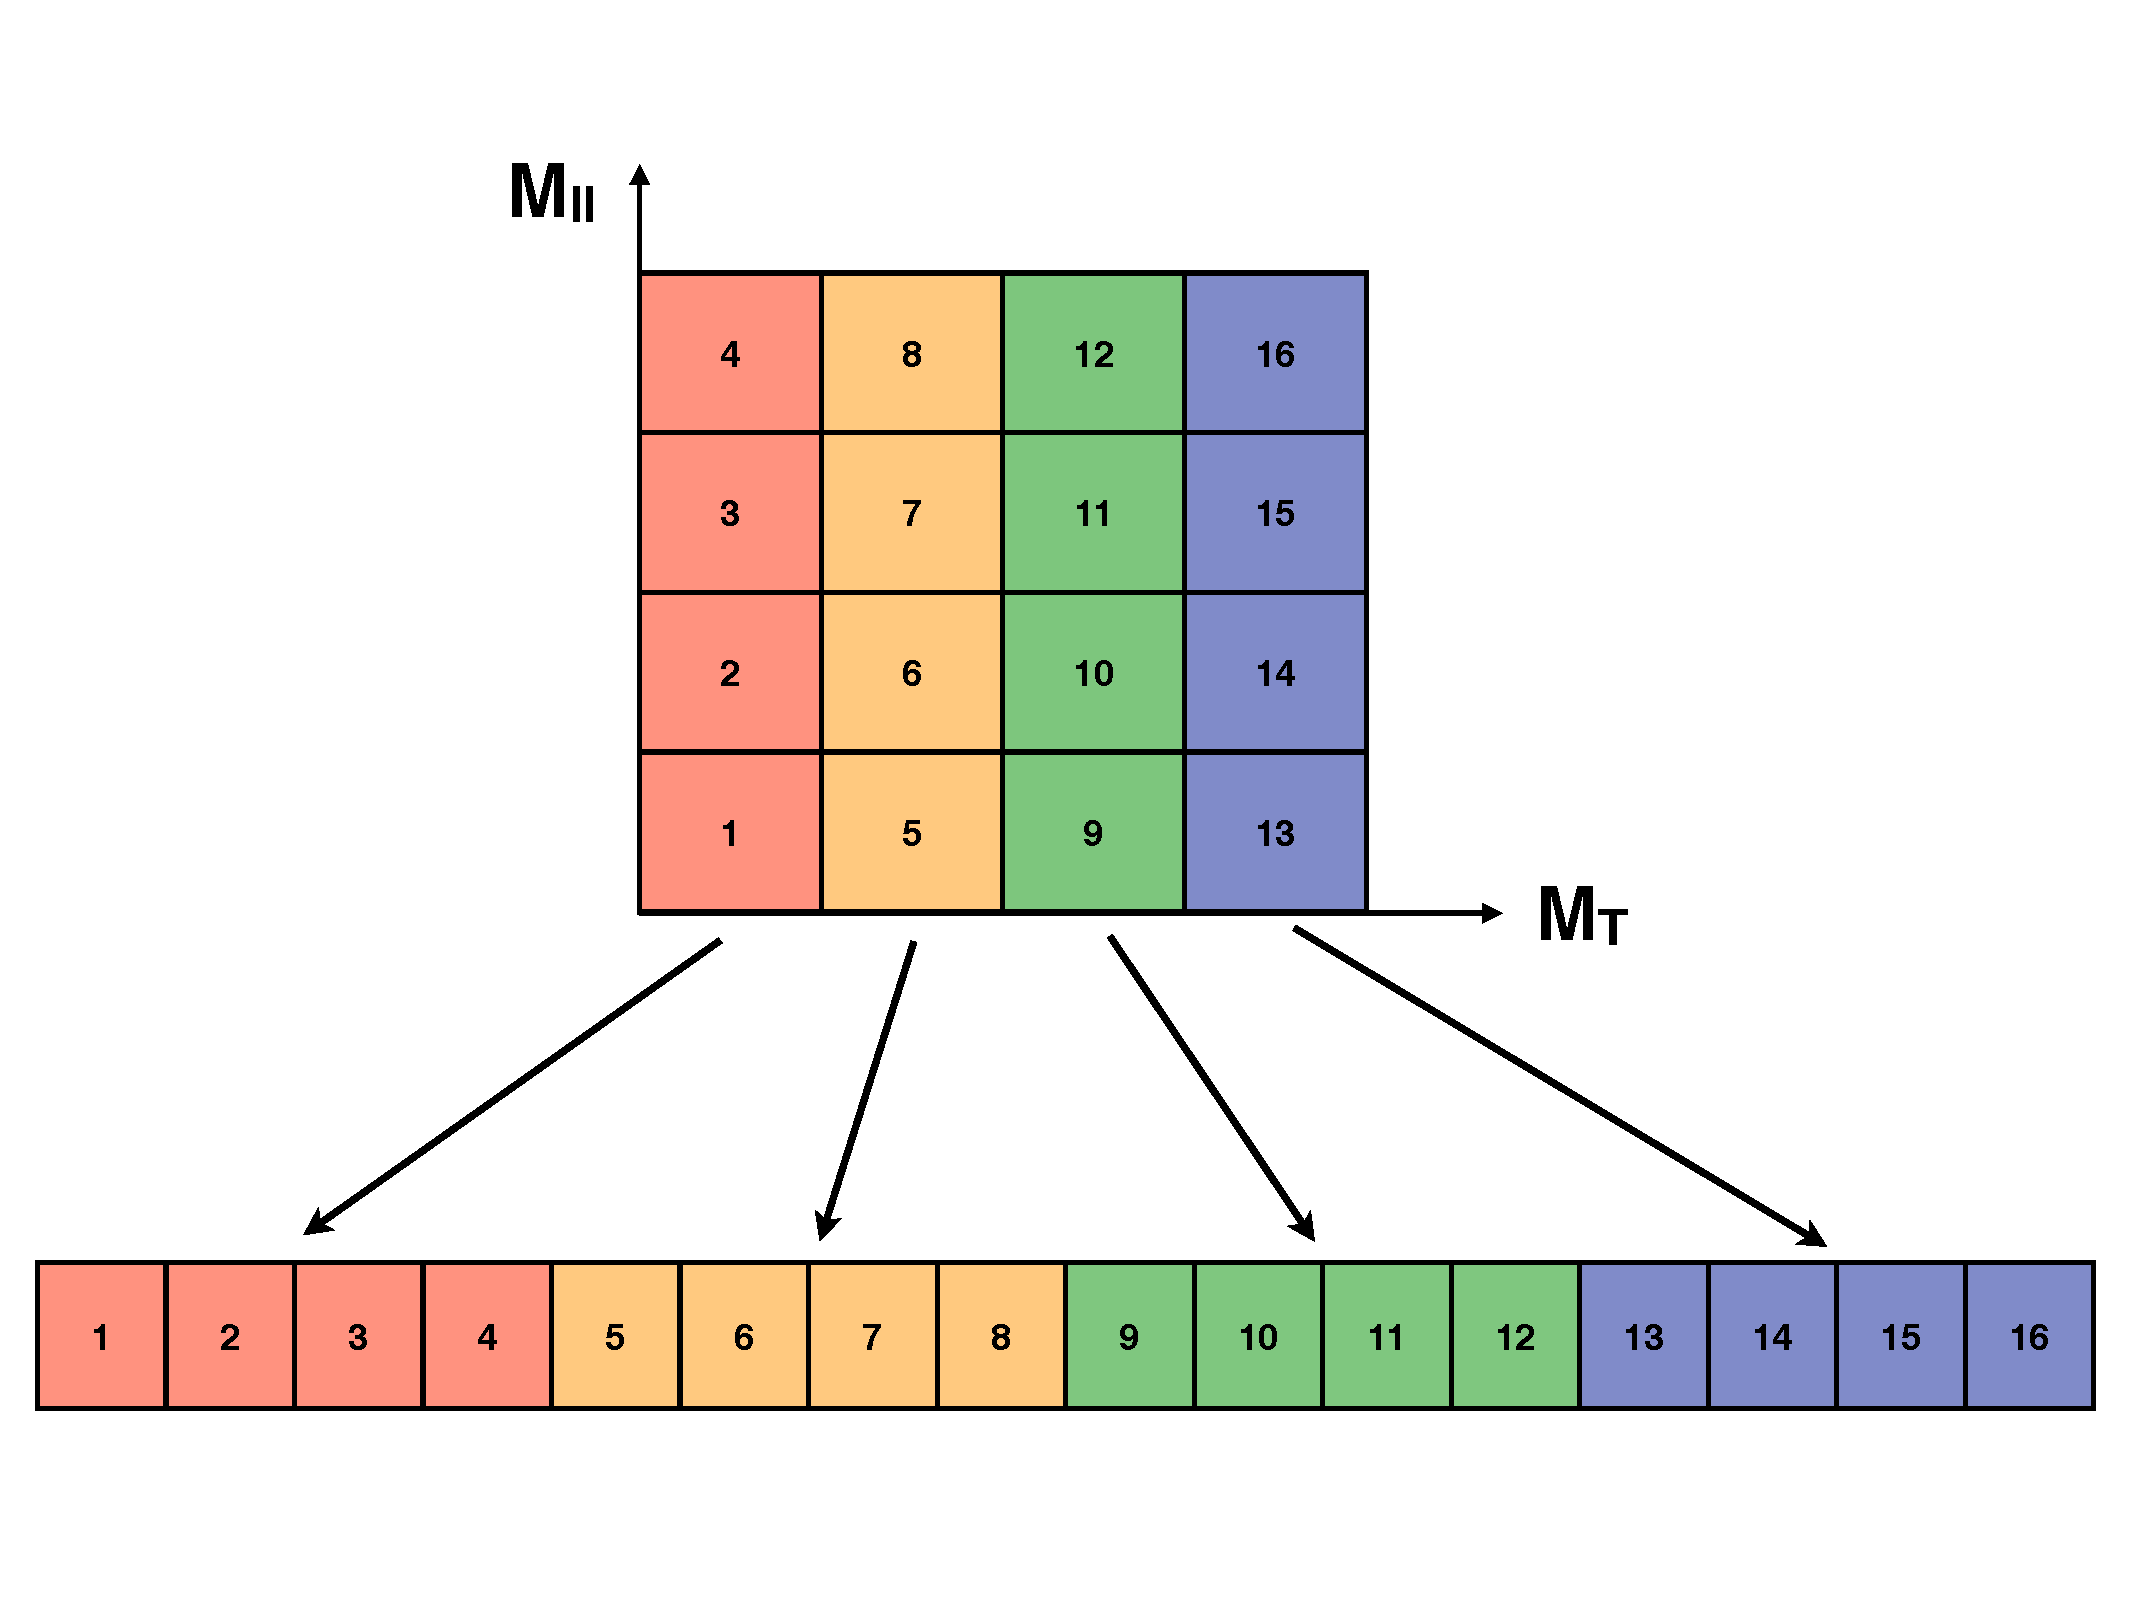
\includegraphics[width=0.8\textwidth]{figures/unrolling_schematic.pdf}
	\caption{ Schematic of how unrolling is done from 4x4 2D to 1D histogram. 
			  The numbers in the 2D and 1D histograms indicate the same bins.} 
  	\label{fig:unrolling_sch}
\end{figure}

Figure~\ref{fig:unrolling_sch} shows how the unrolling is done.
In the case of a 4x4 2D template, the first column in the 2D histogram 
becomes the 1st - 4th bins in the 1D histogram. The second column becomes 
5th - 8th bins in the 1D. Same thing goes until the last column.  
Figure~\ref{fig:unrolling_ex} shows an example of 2D template and
the corresponding unrolled template.

\begin{figure}[htp]
	\centering
	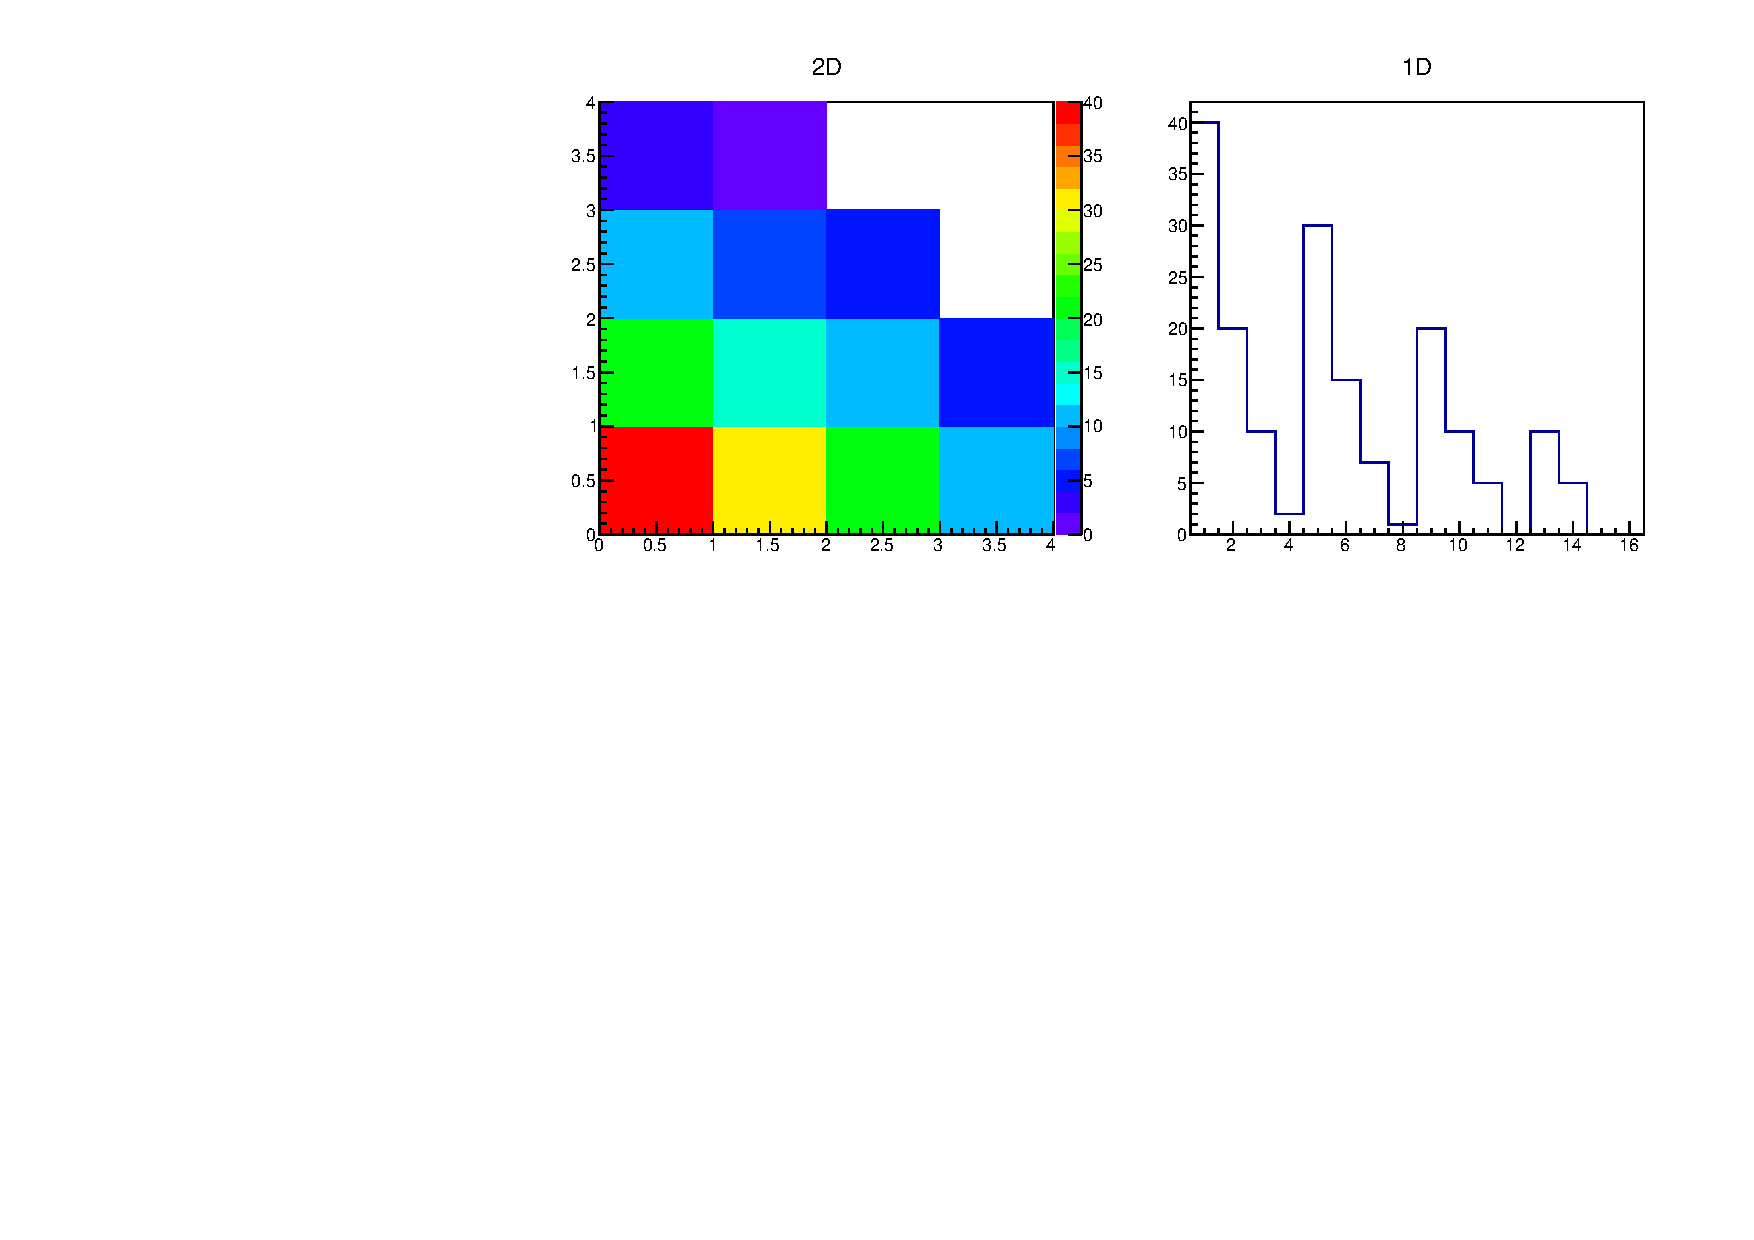
\includegraphics[width=0.8\textwidth]{figures/unrolling_example.pdf}
	\caption{ Example of how unrolling is done from 4x4 2D to 1D histogram.} 
  	\label{fig:unrolling_ex}
\end{figure}


  
  \subsection{Templates}
  \label{sec:templates}
  Once bin size and range are decided, we need to check if the templates 
for all signal and background processes are reasonably filled 
to avoid any biases due to poor statistics. [ref?] 

\begin{figure}[!hbtp]
	
	%
	\centering
	\subfigure[Signal]{
	\centering
	\label{subfig:template_signal_125}
		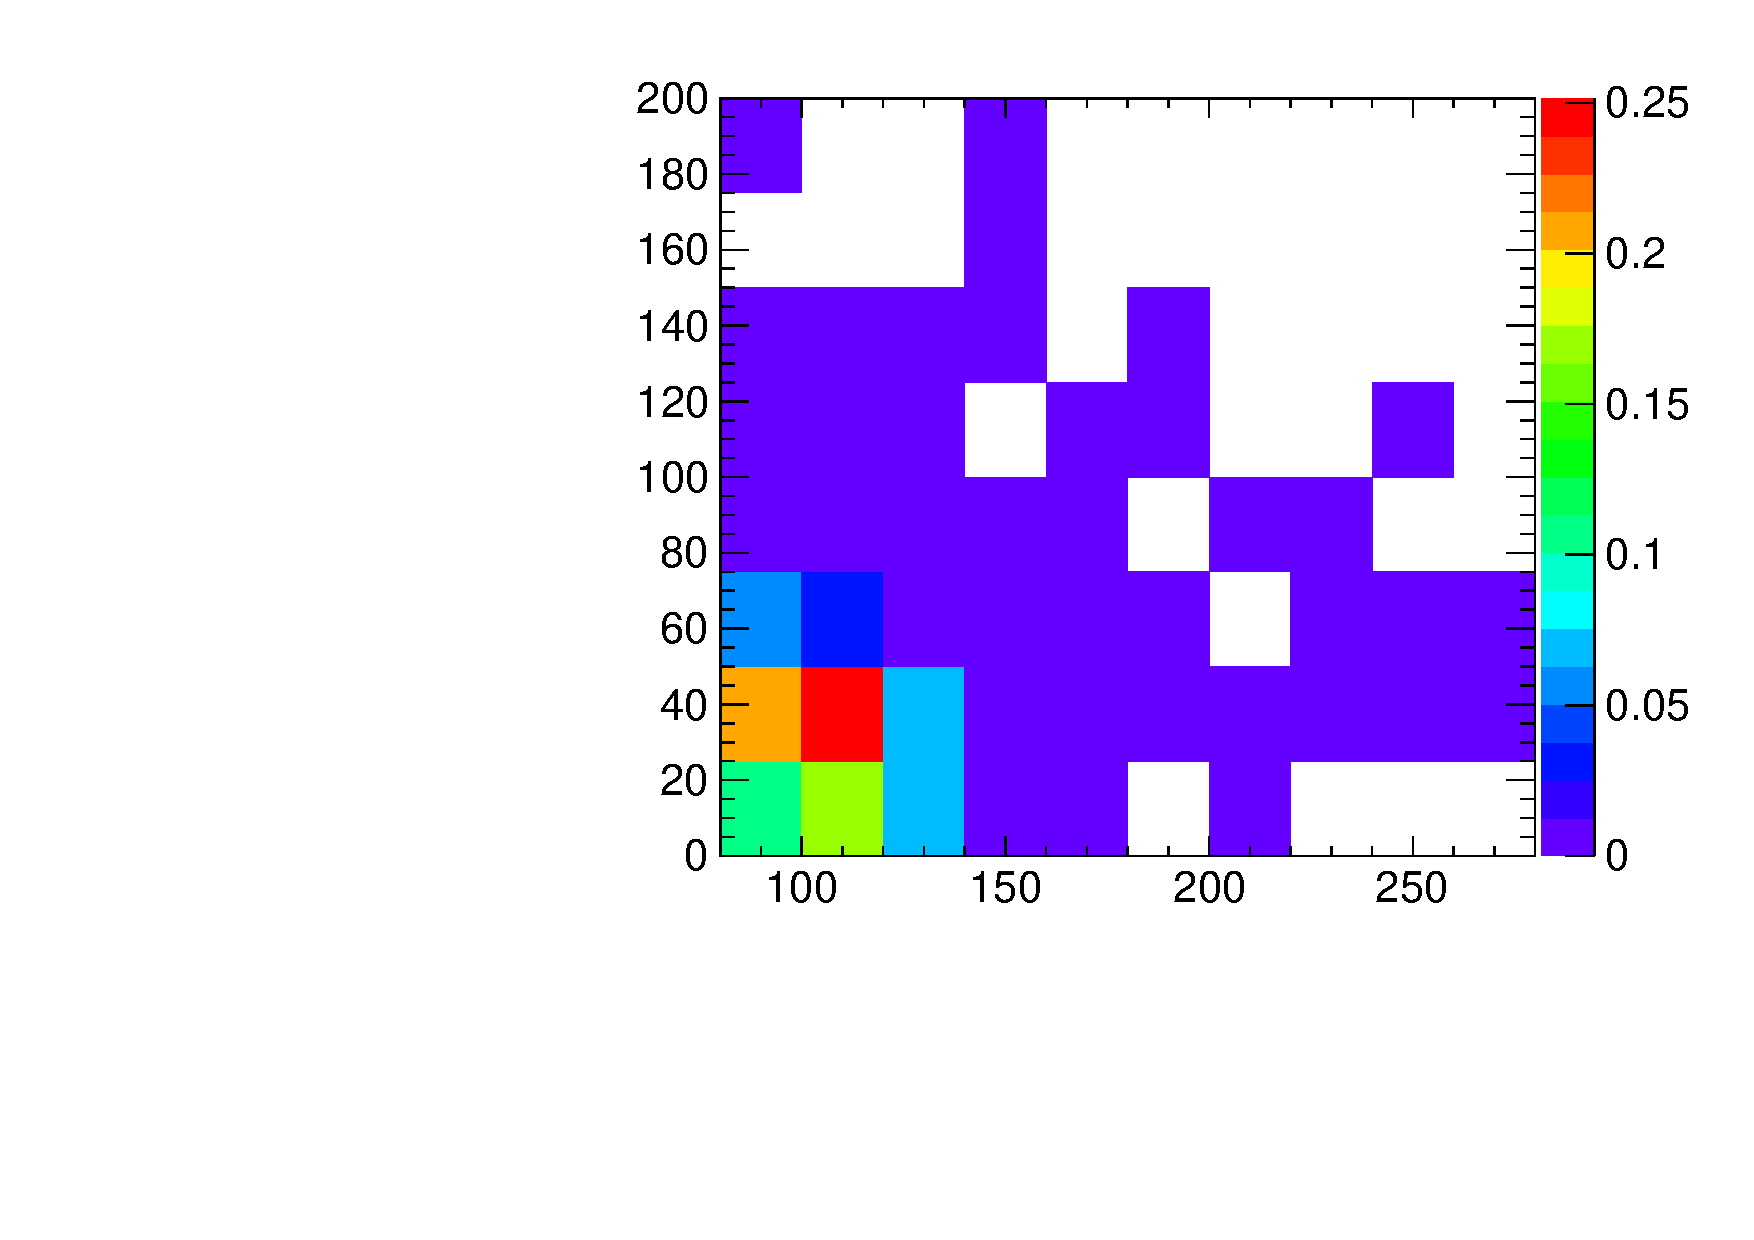
\includegraphics[width=.35\textwidth]{figures/templates/sig_2D_mH125_0j_of.pdf}
	}
	\subfigure[Signal statistical uncertainty]{
	\centering
	\label{subfig:template_signalerr_125}
		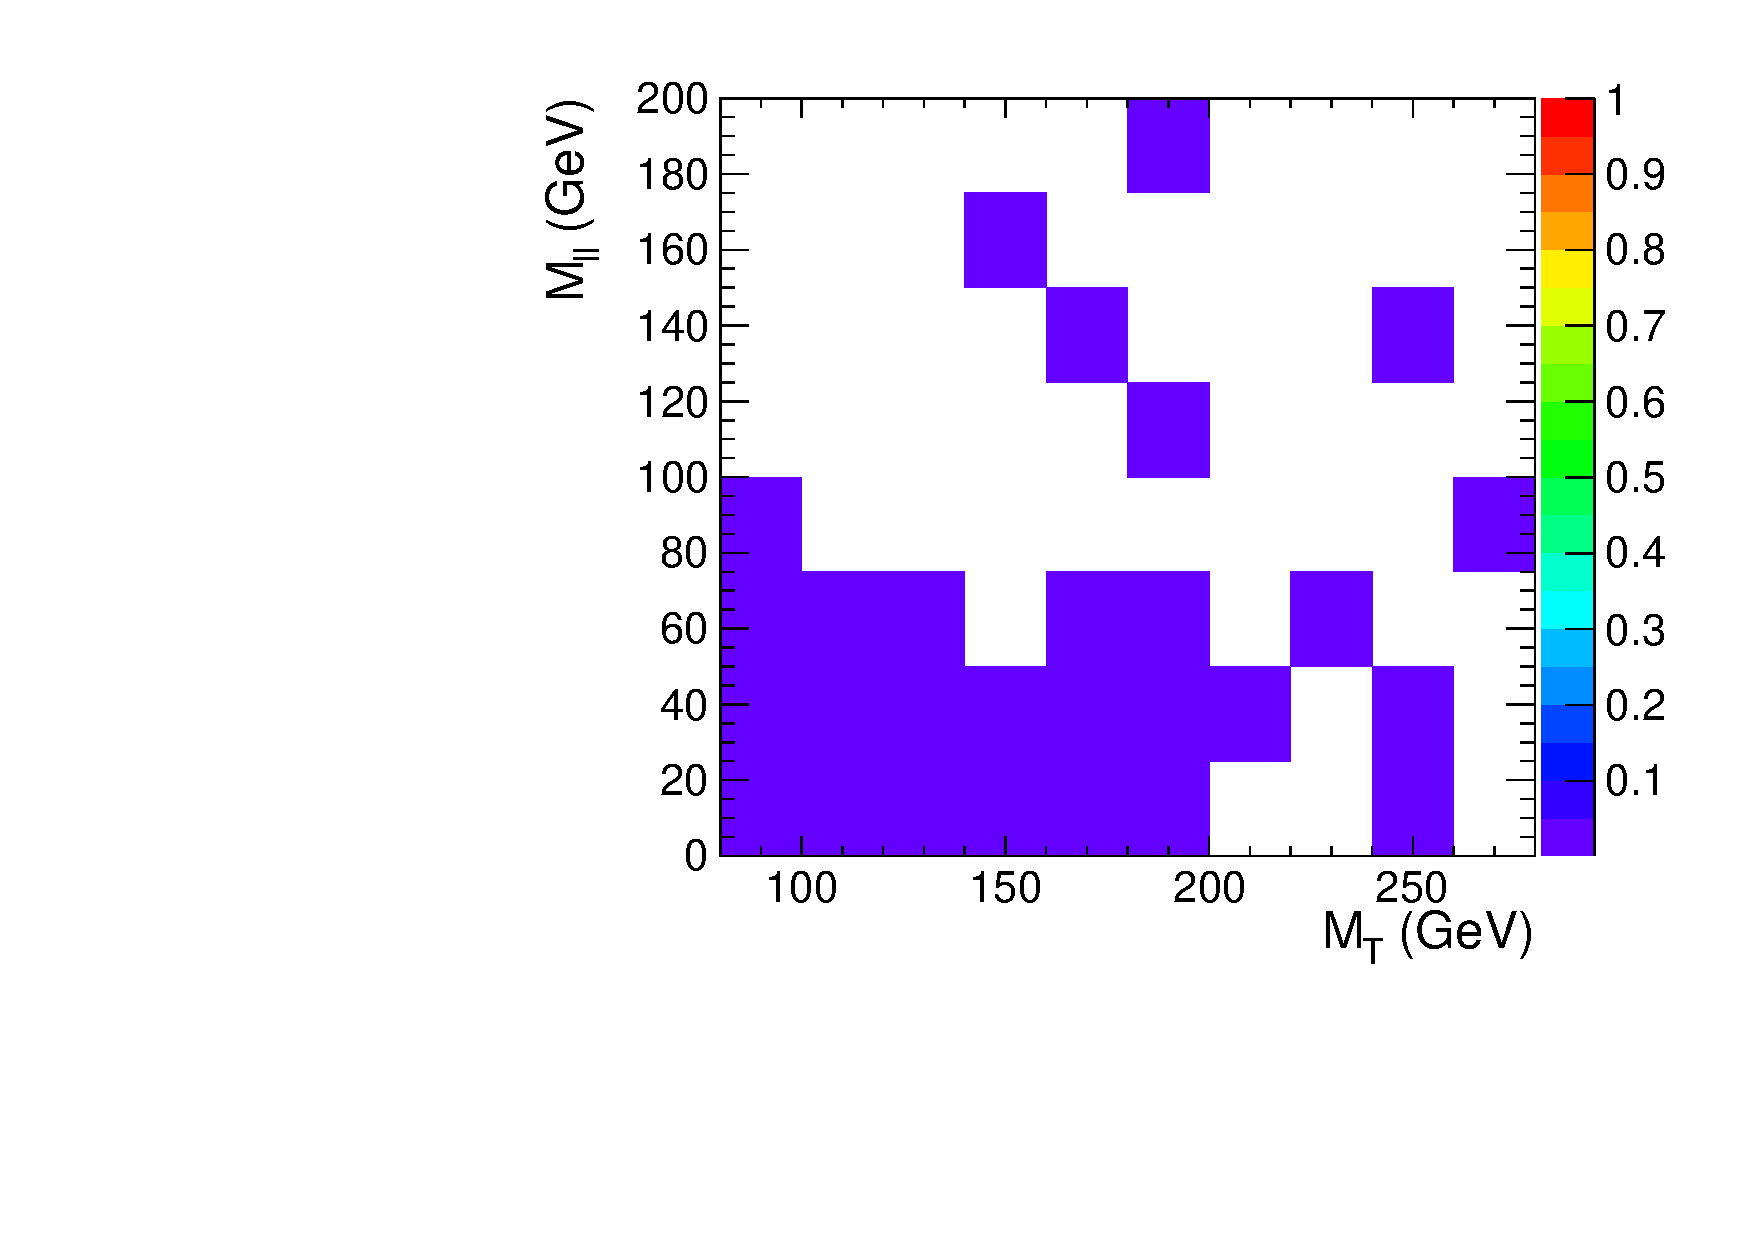
\includegraphics[width=.35\textwidth]{figures/templates/sigerr_2D_mH125_0j_of.pdf}
	}
	
	%
	\centering
	\subfigure[qqWW]{
	\centering
	\label{subfig:template_qqWW_125}
		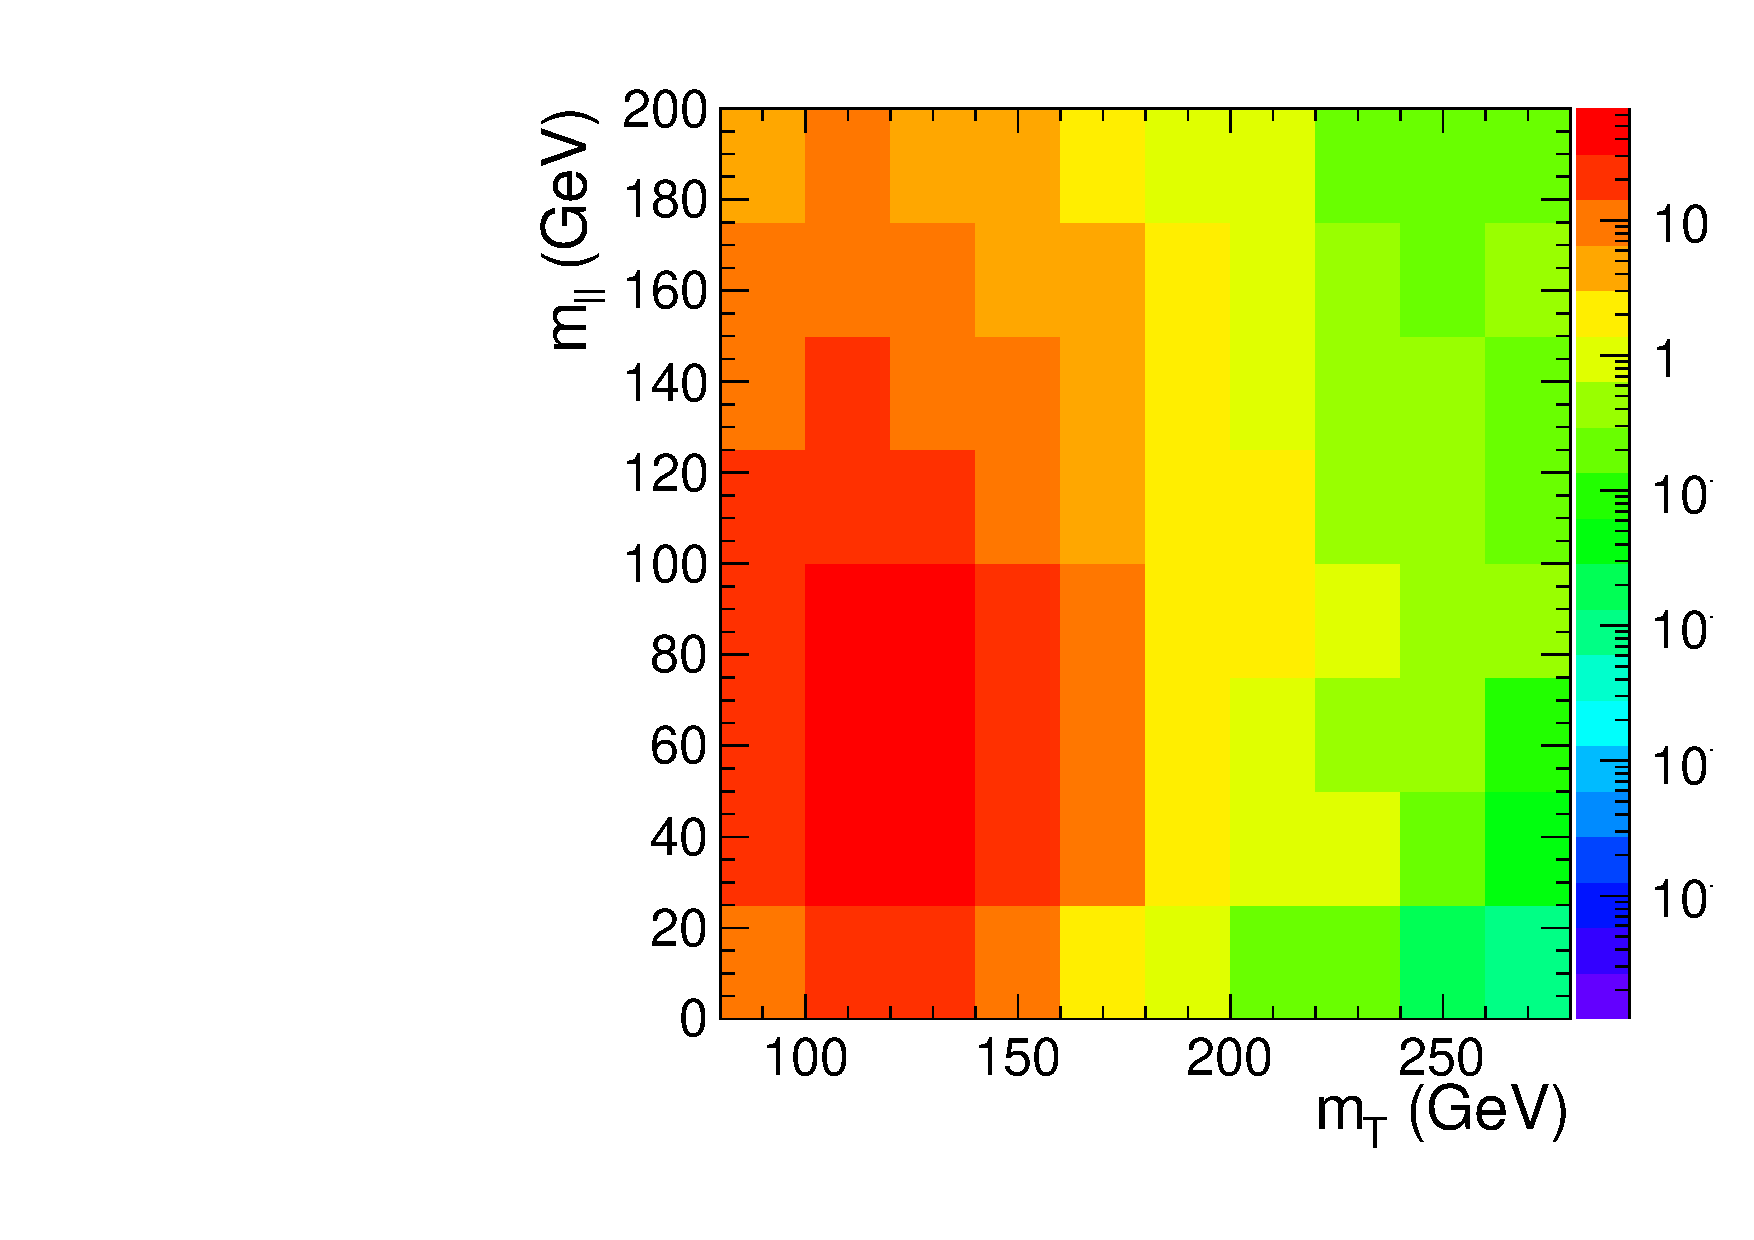
\includegraphics[width=.35\textwidth]{figures/templates/qqWW_2D_mH125_0j_of.pdf}
	}
	\subfigure[qqWW statistical uncertainty]{
	\centering
	\label{subfig:template_qqWWerr_125}
		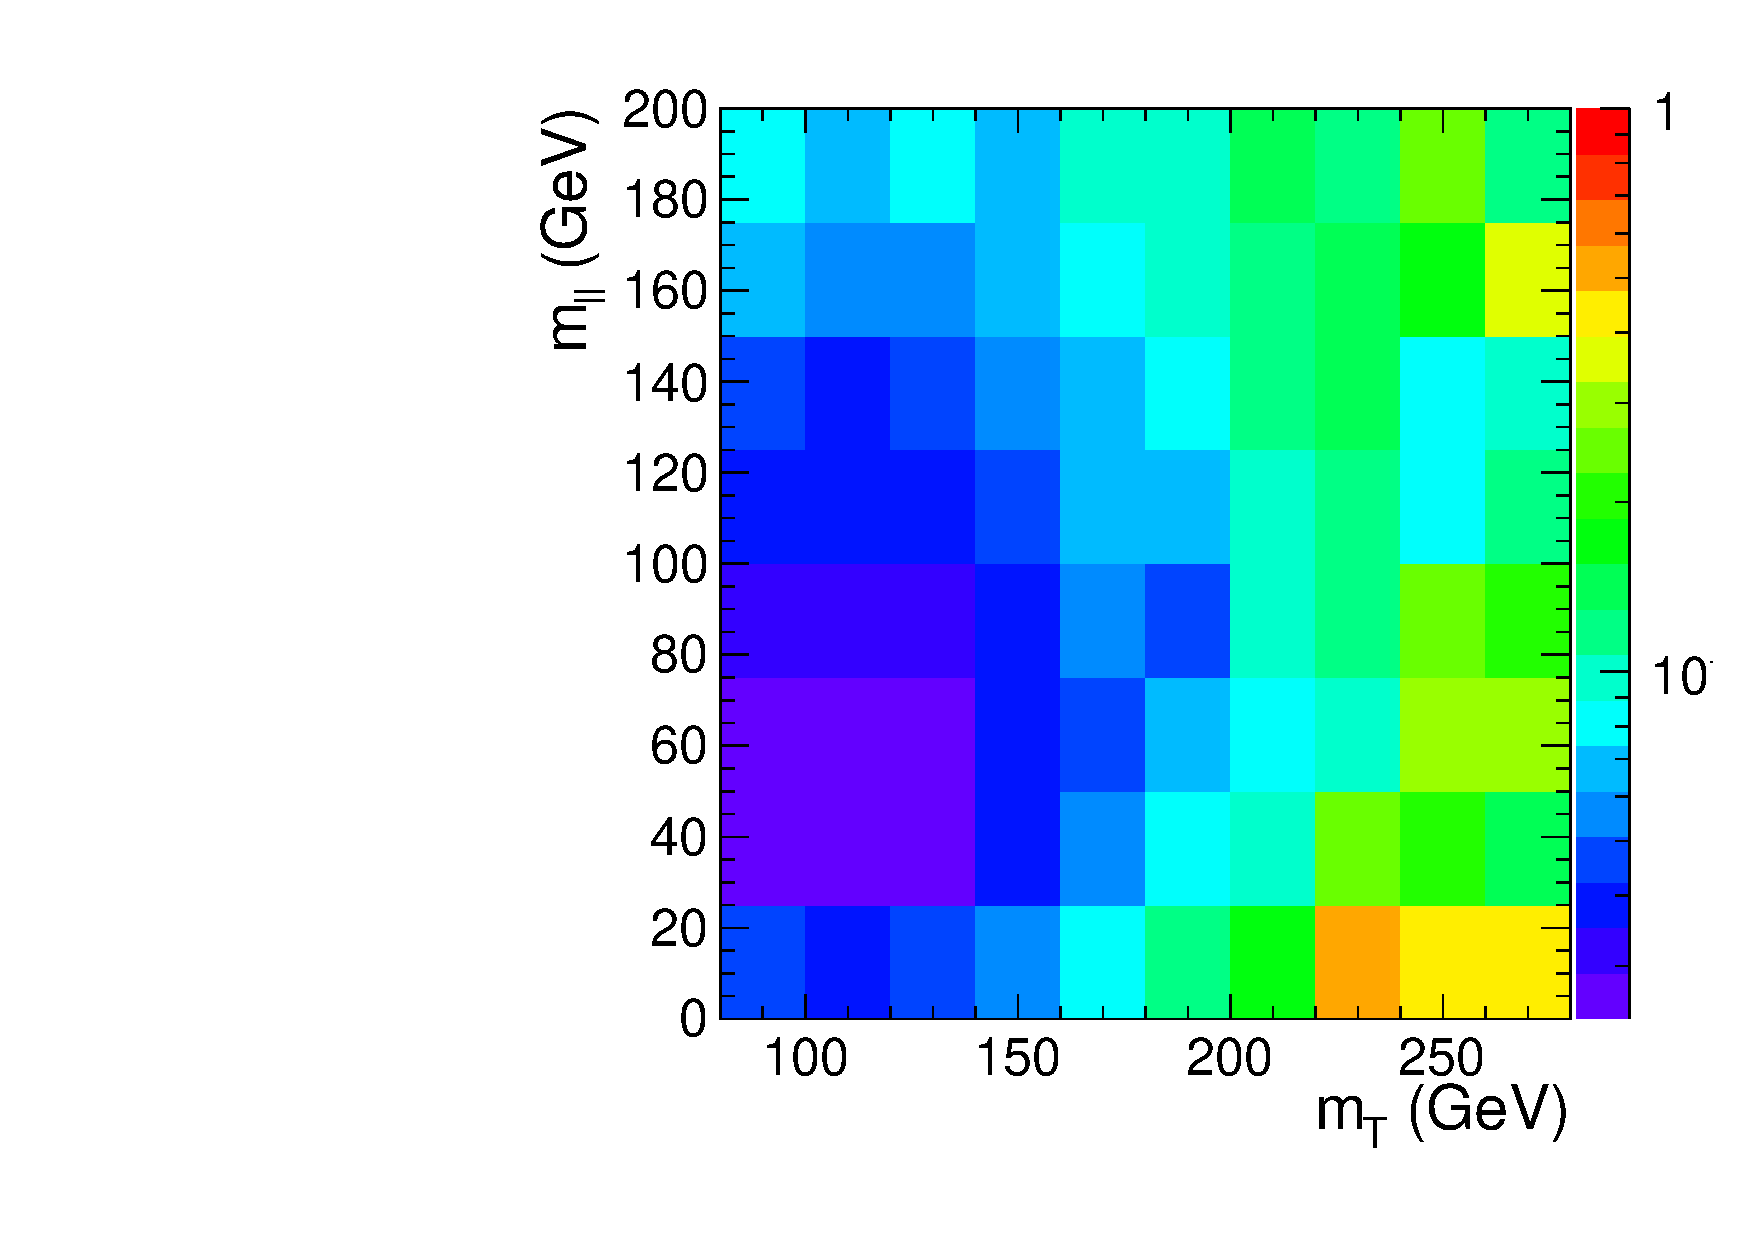
\includegraphics[width=.35\textwidth]{figures/templates/qqWWerr_2D_mH125_0j_of.pdf}
	}

	%
	\centering
	\subfigure[ggWW]{
	\centering
	\label{subfig:template_ggWW_125}
		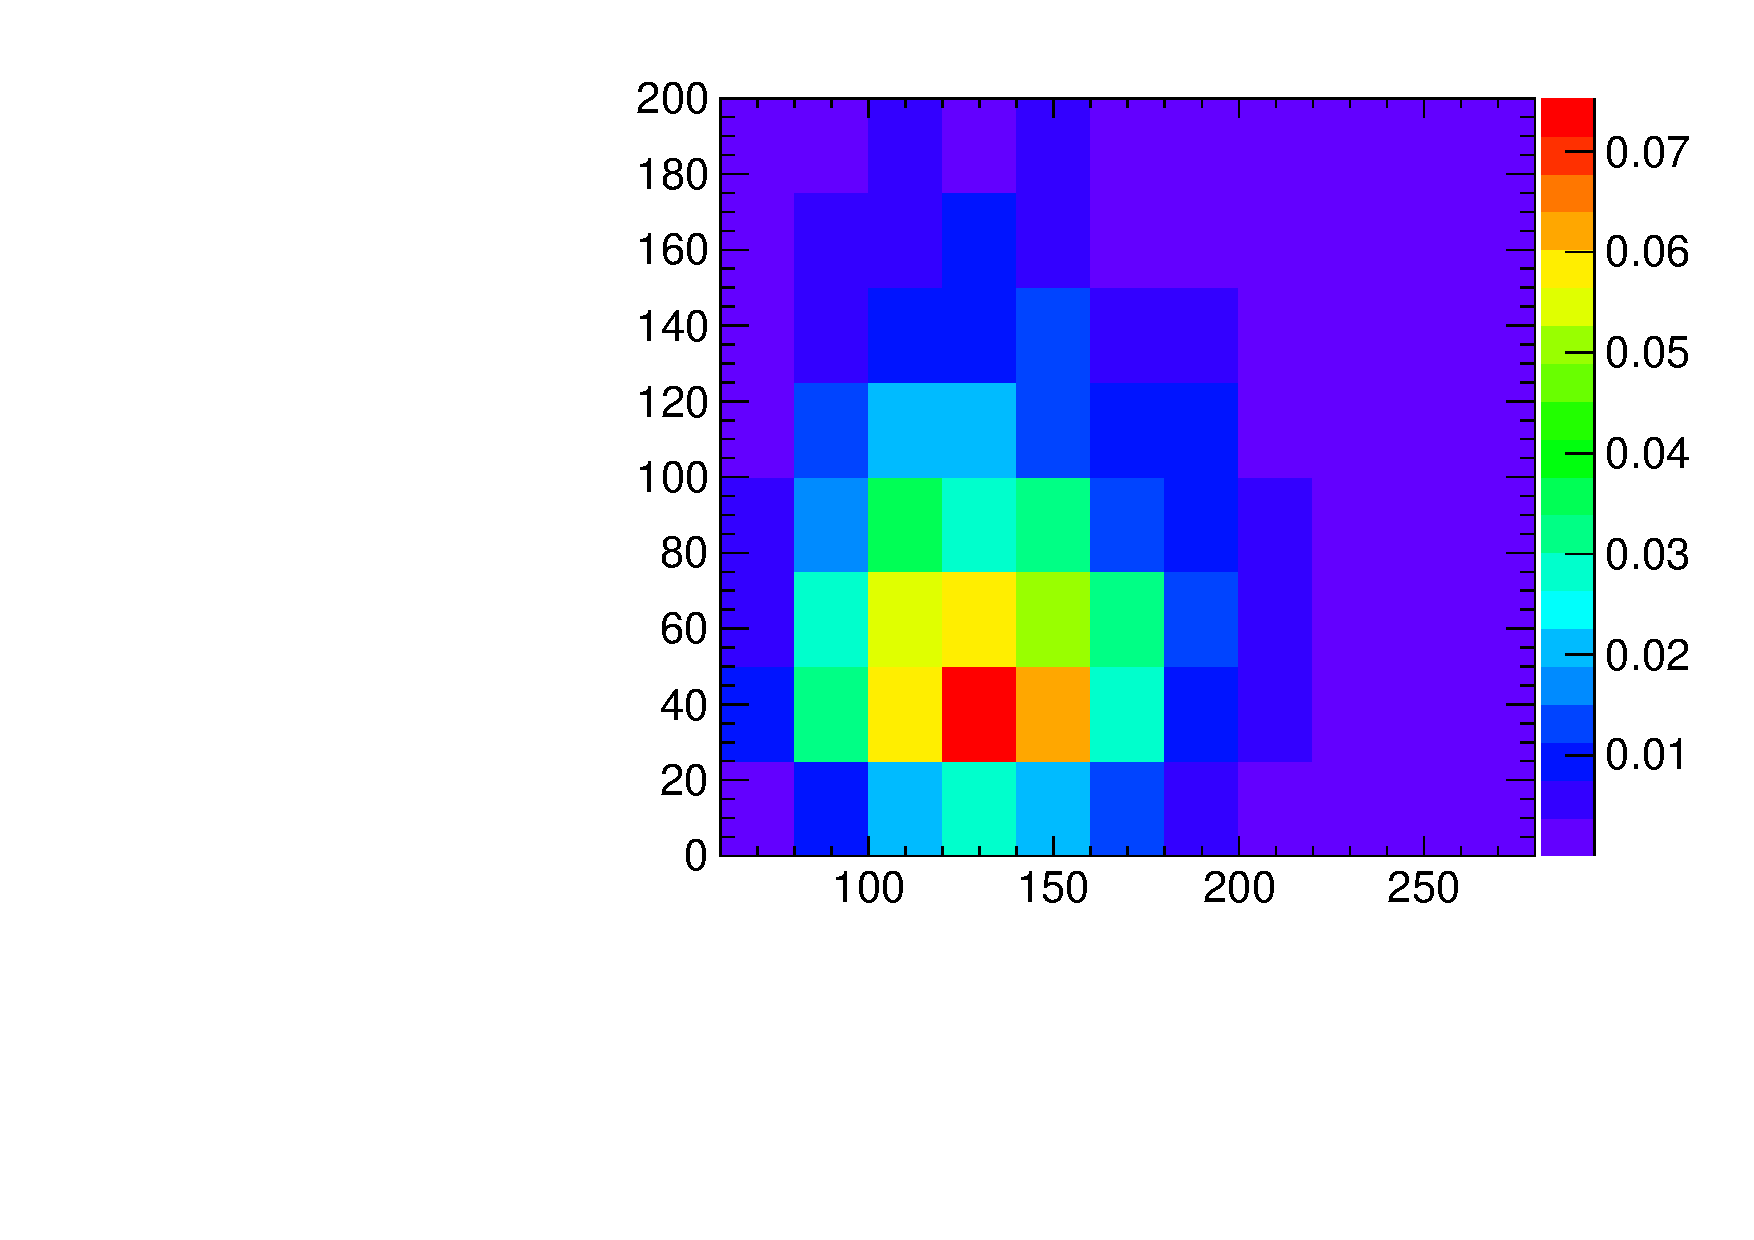
\includegraphics[width=.35\textwidth]{figures/templates/ggWW_2D_mH125_0j_of.pdf}
	}
	\subfigure[ggWW statistical uncertainty]{
	\centering
	\label{subfig:template_ggWWerr_125}
		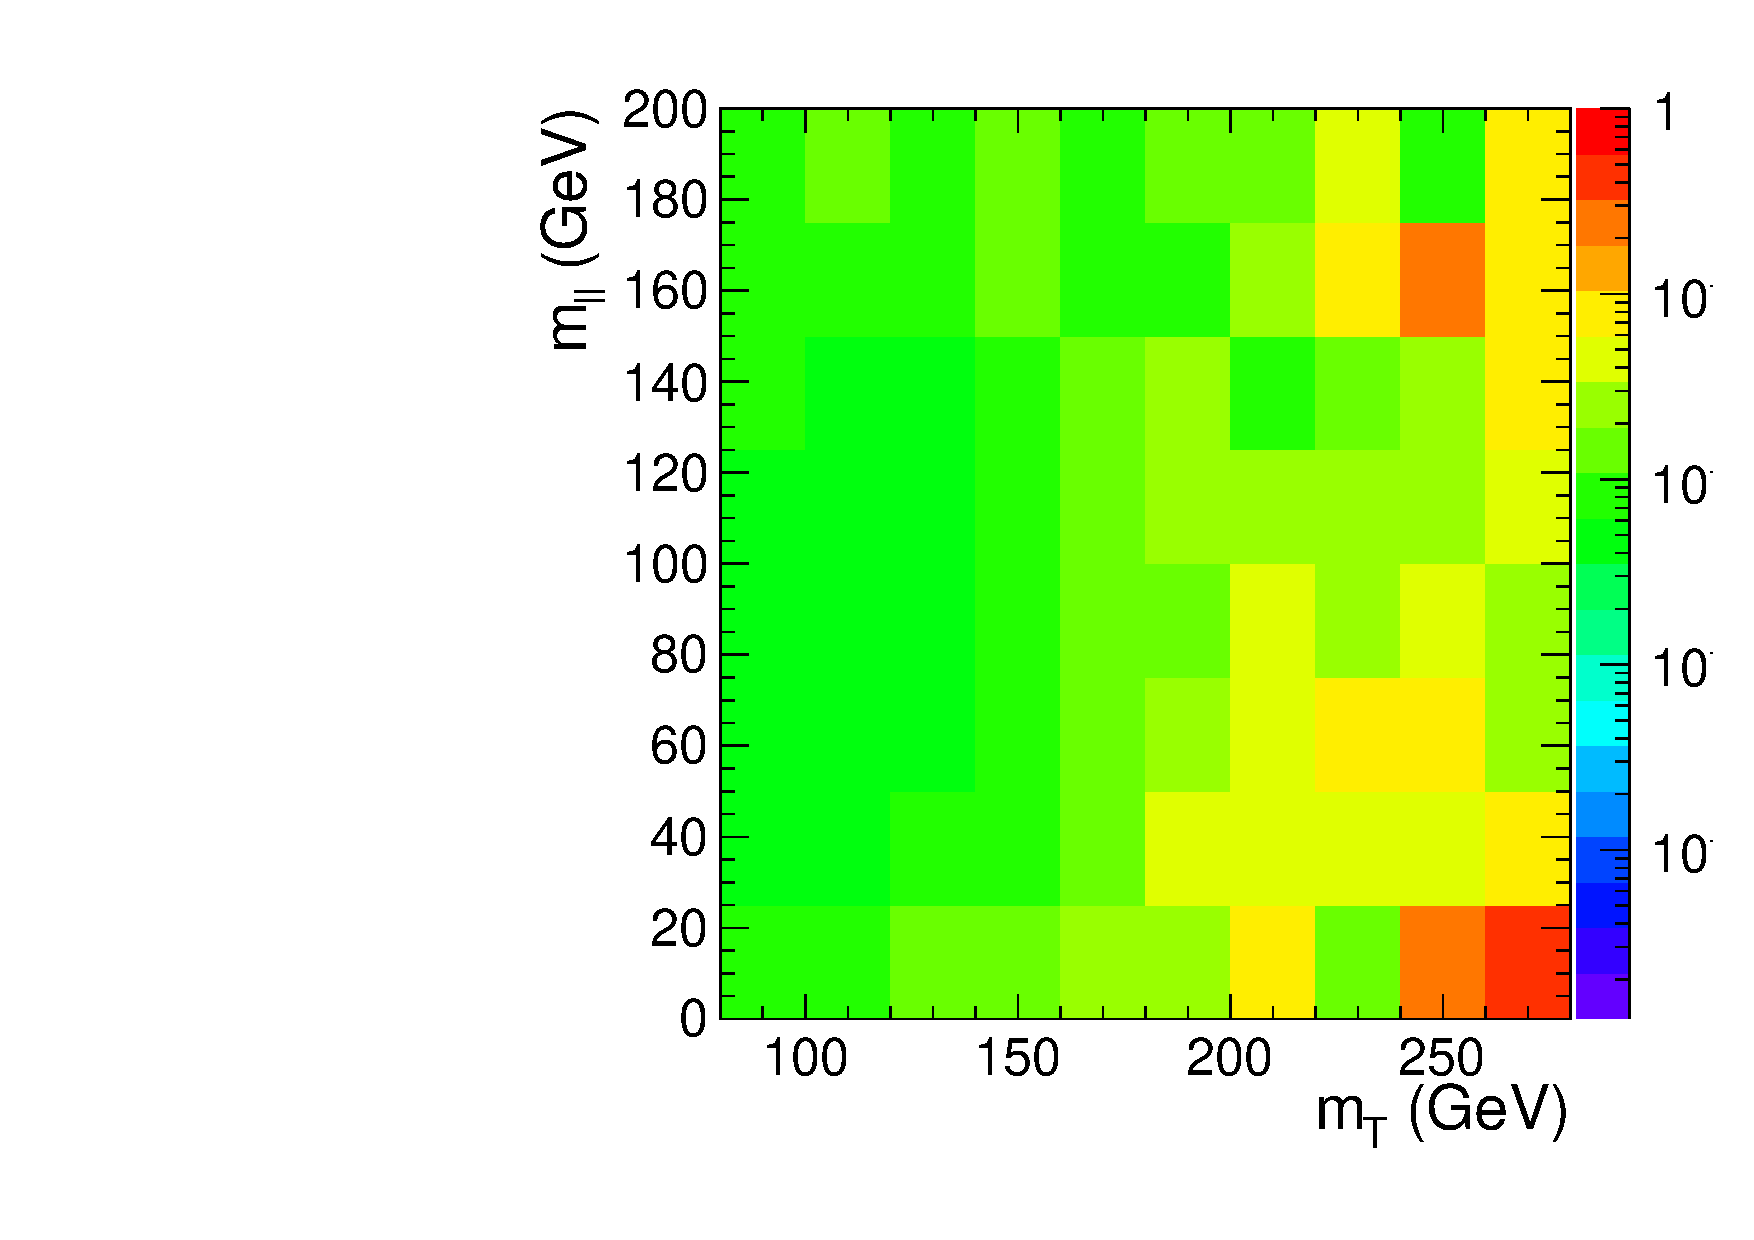
\includegraphics[width=.35\textwidth]{figures/templates/ggWWerr_2D_mH125_0j_of.pdf}
	}

	\caption{2D templates at \mHi = 125 \GeV} 
	\label{fig:templates_125_1}

\end{figure}

\begin{figure}[!hbtp]
	
	%
	\centering
	\subfigure[Wjets]{
	\centering
	\label{subfig:template_Wjets_125}
		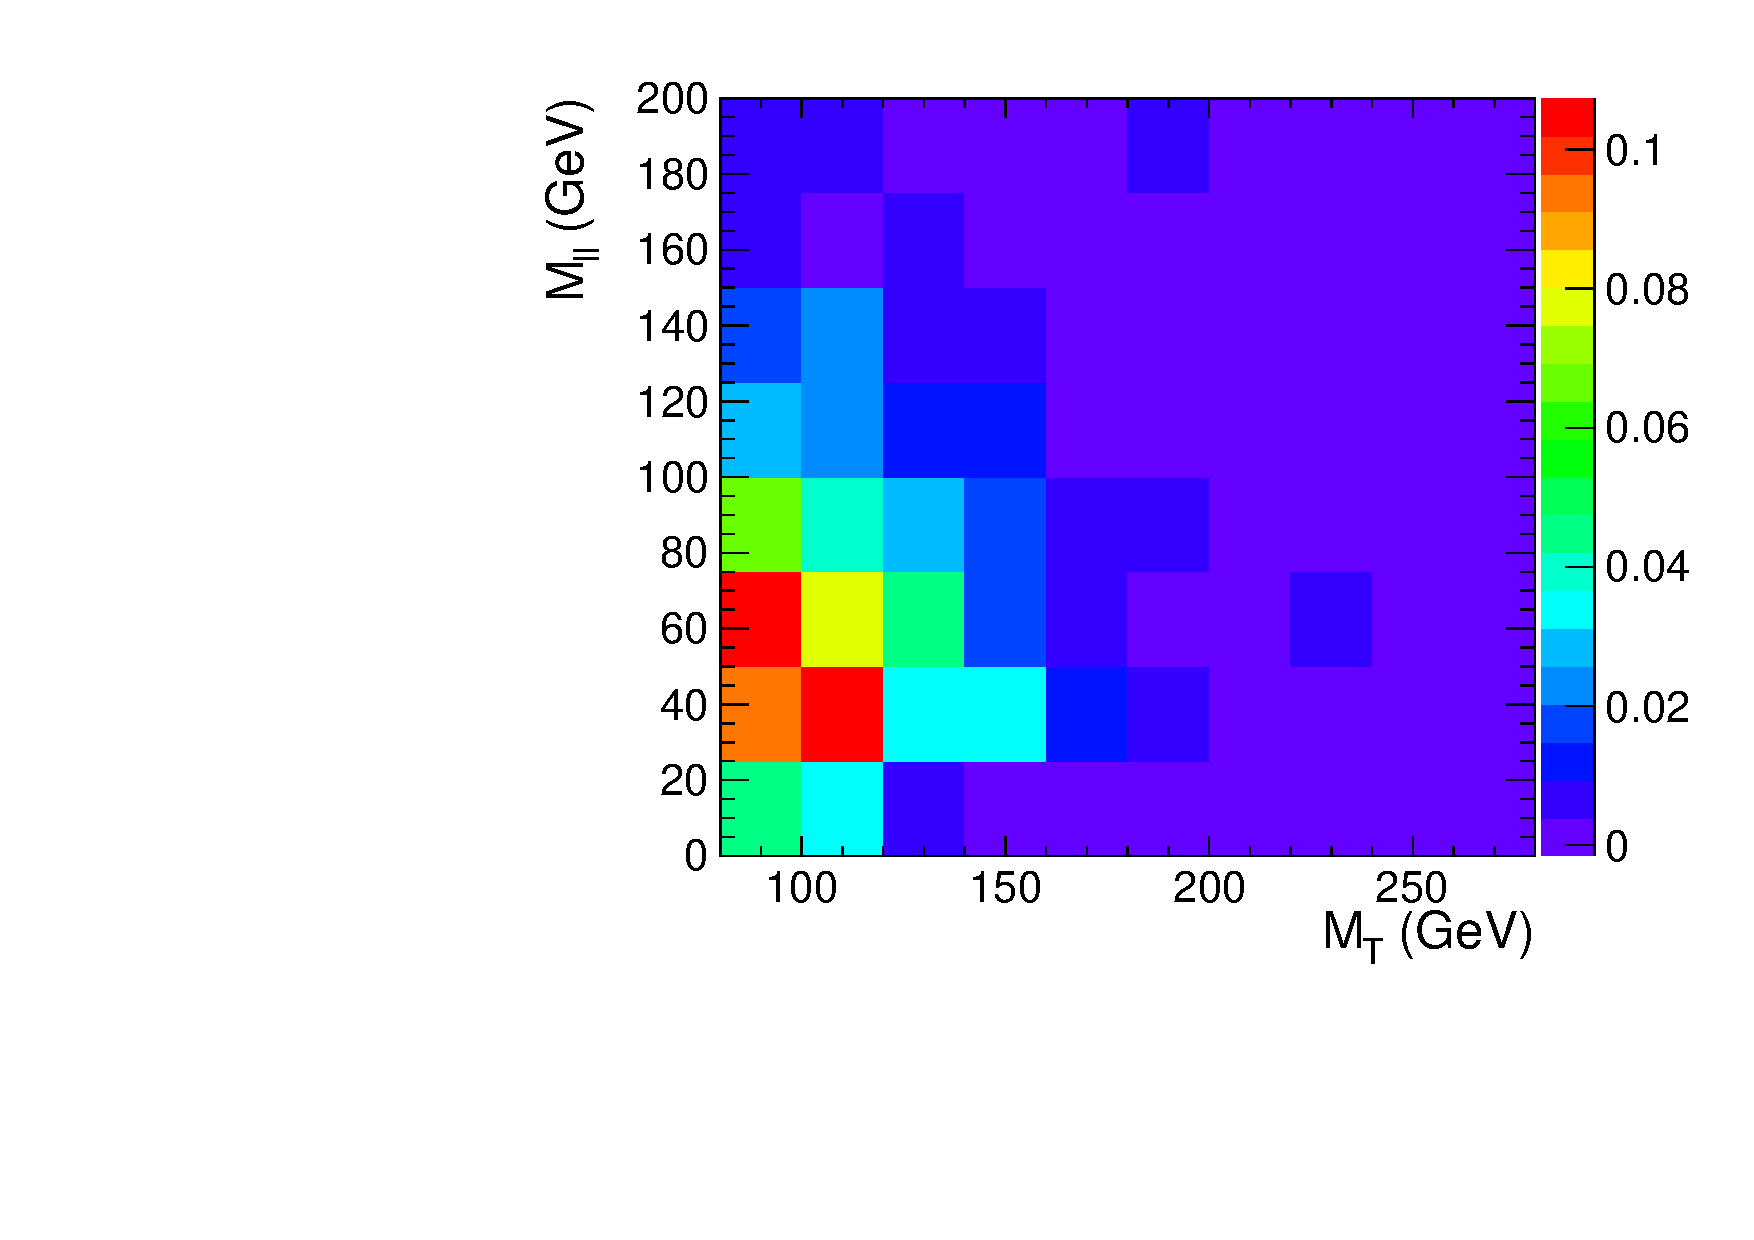
\includegraphics[width=.35\textwidth]{figures/templates/Wjets_2D_mH125_0j_of.pdf}
	}
	\subfigure[Wjets statistical uncertainty]{
	\centering
	\label{subfig:template_Wjetserr_125}
		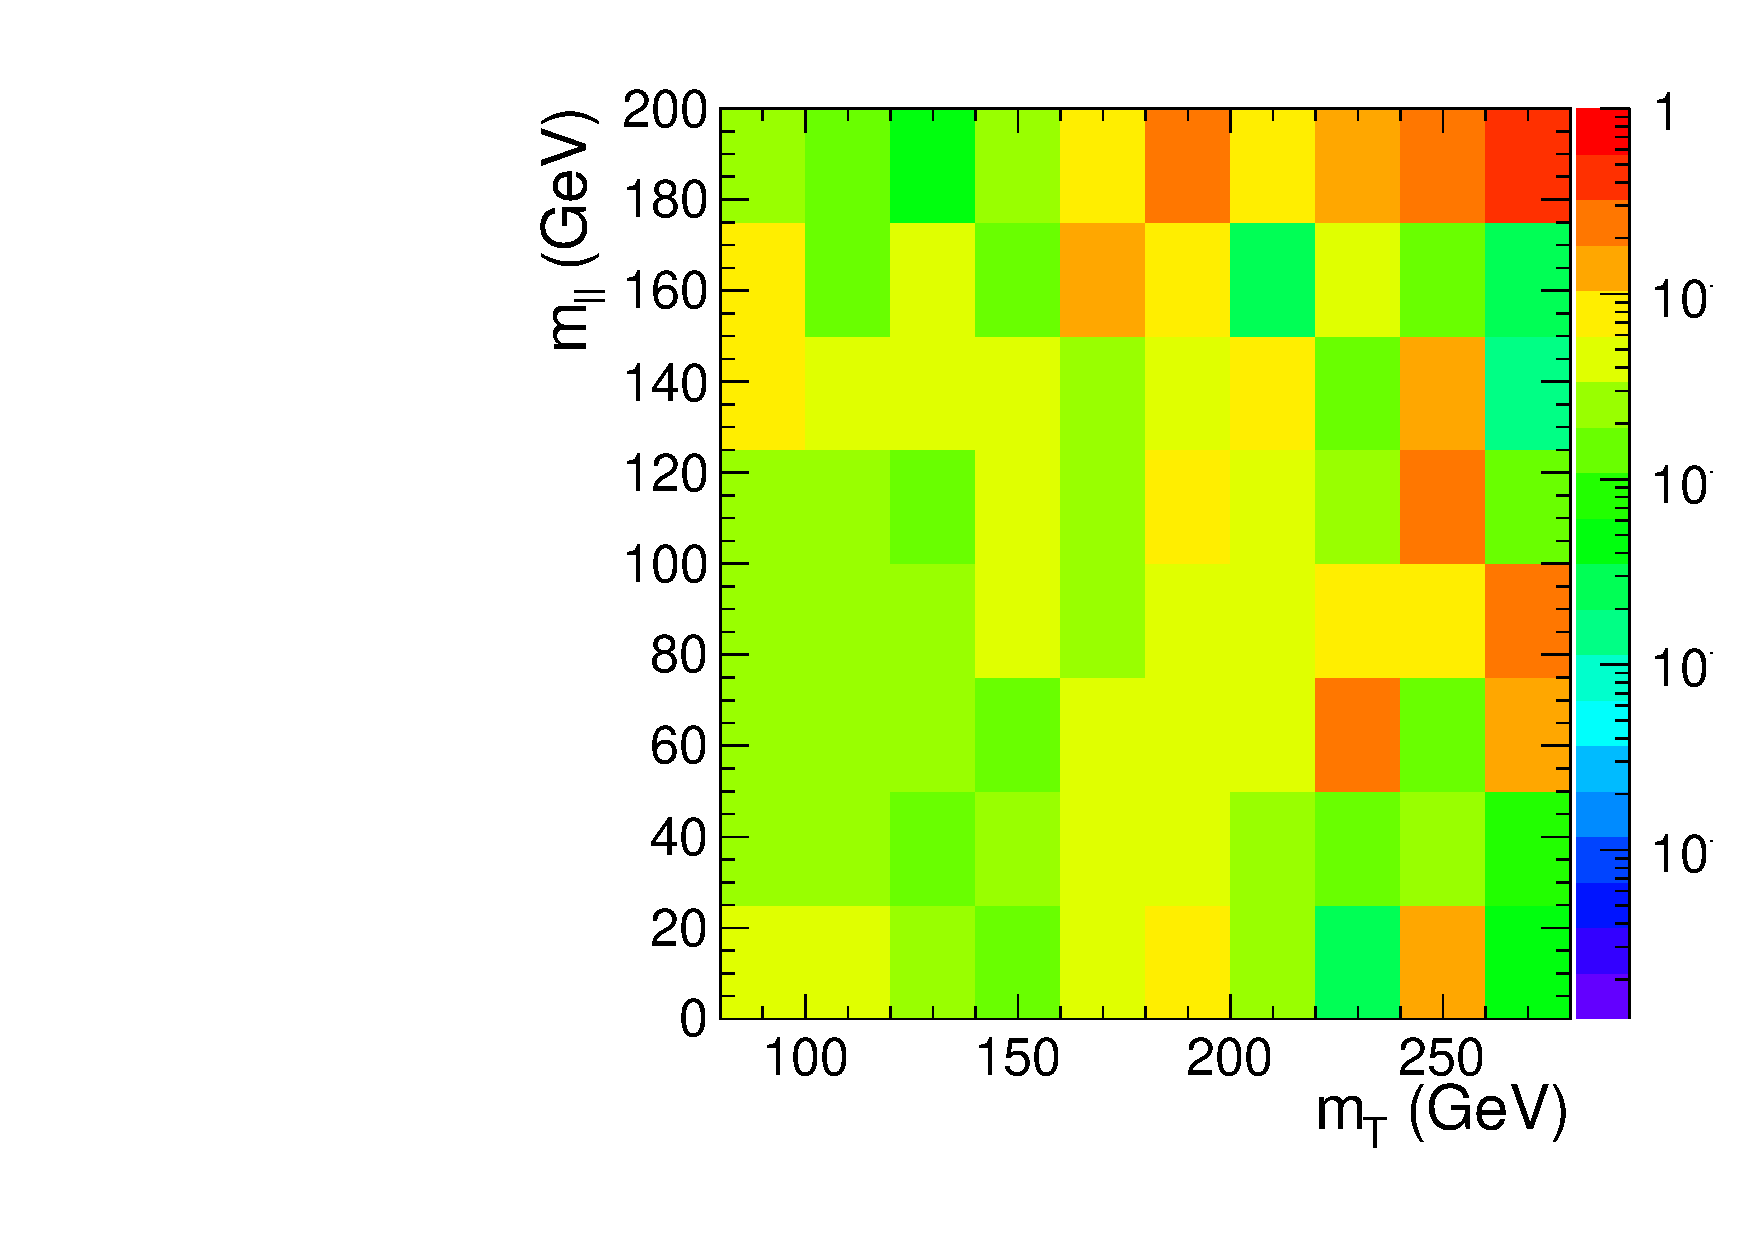
\includegraphics[width=.35\textwidth]{figures/templates/Wjetserr_2D_mH125_0j_of.pdf}
	}
	
	%
	\centering
	\subfigure[Top]{
	\centering
	\label{subfig:template_Top_125}
		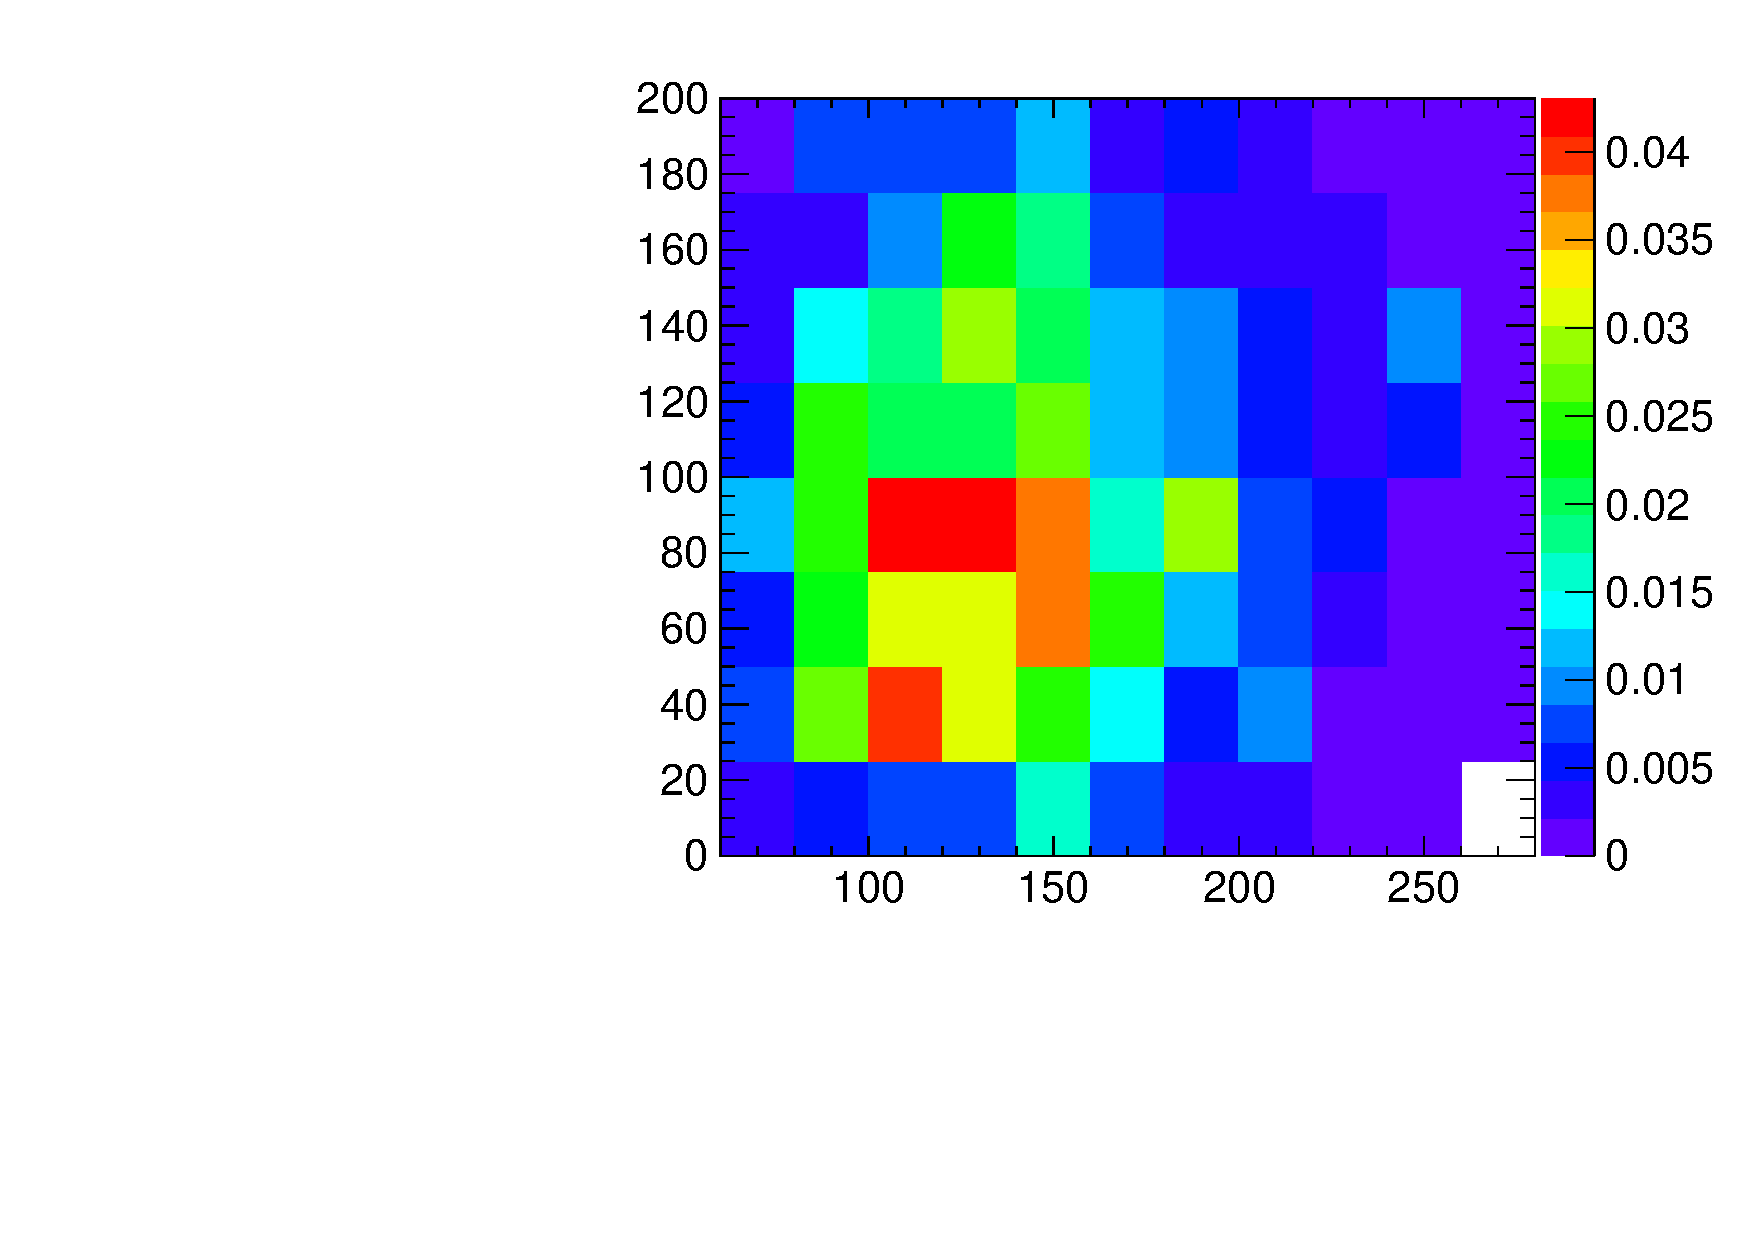
\includegraphics[width=.35\textwidth]{figures/templates/Top_2D_mH125_0j_of.pdf}
	}
	\subfigure[Top statistical uncertainty]{
	\centering
	\label{subfig:template_Toperr_125}
		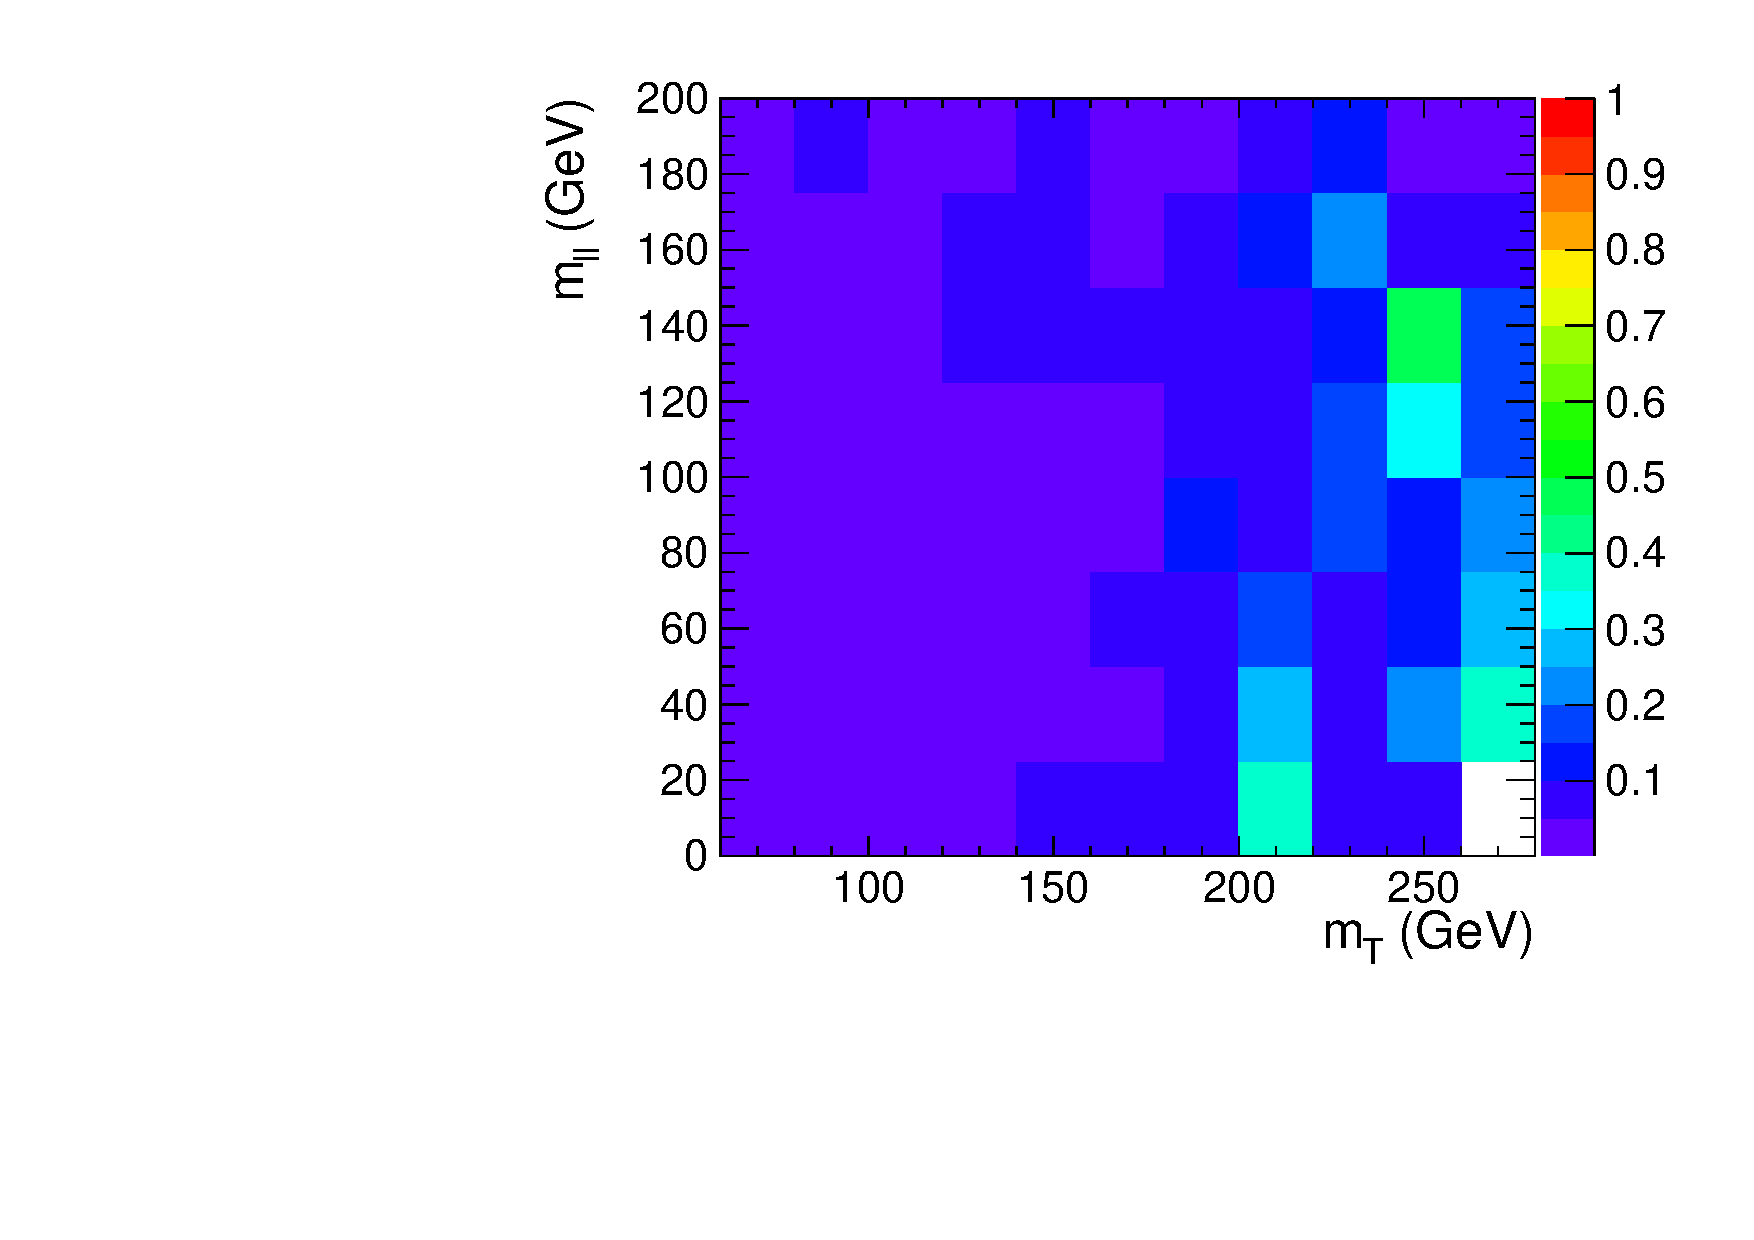
\includegraphics[width=.35\textwidth]{figures/templates/Toperr_2D_mH125_0j_of.pdf}
	}

	%
	\centering
	\subfigure[VV]{
	\centering
	\label{subfig:template_VV_125}
		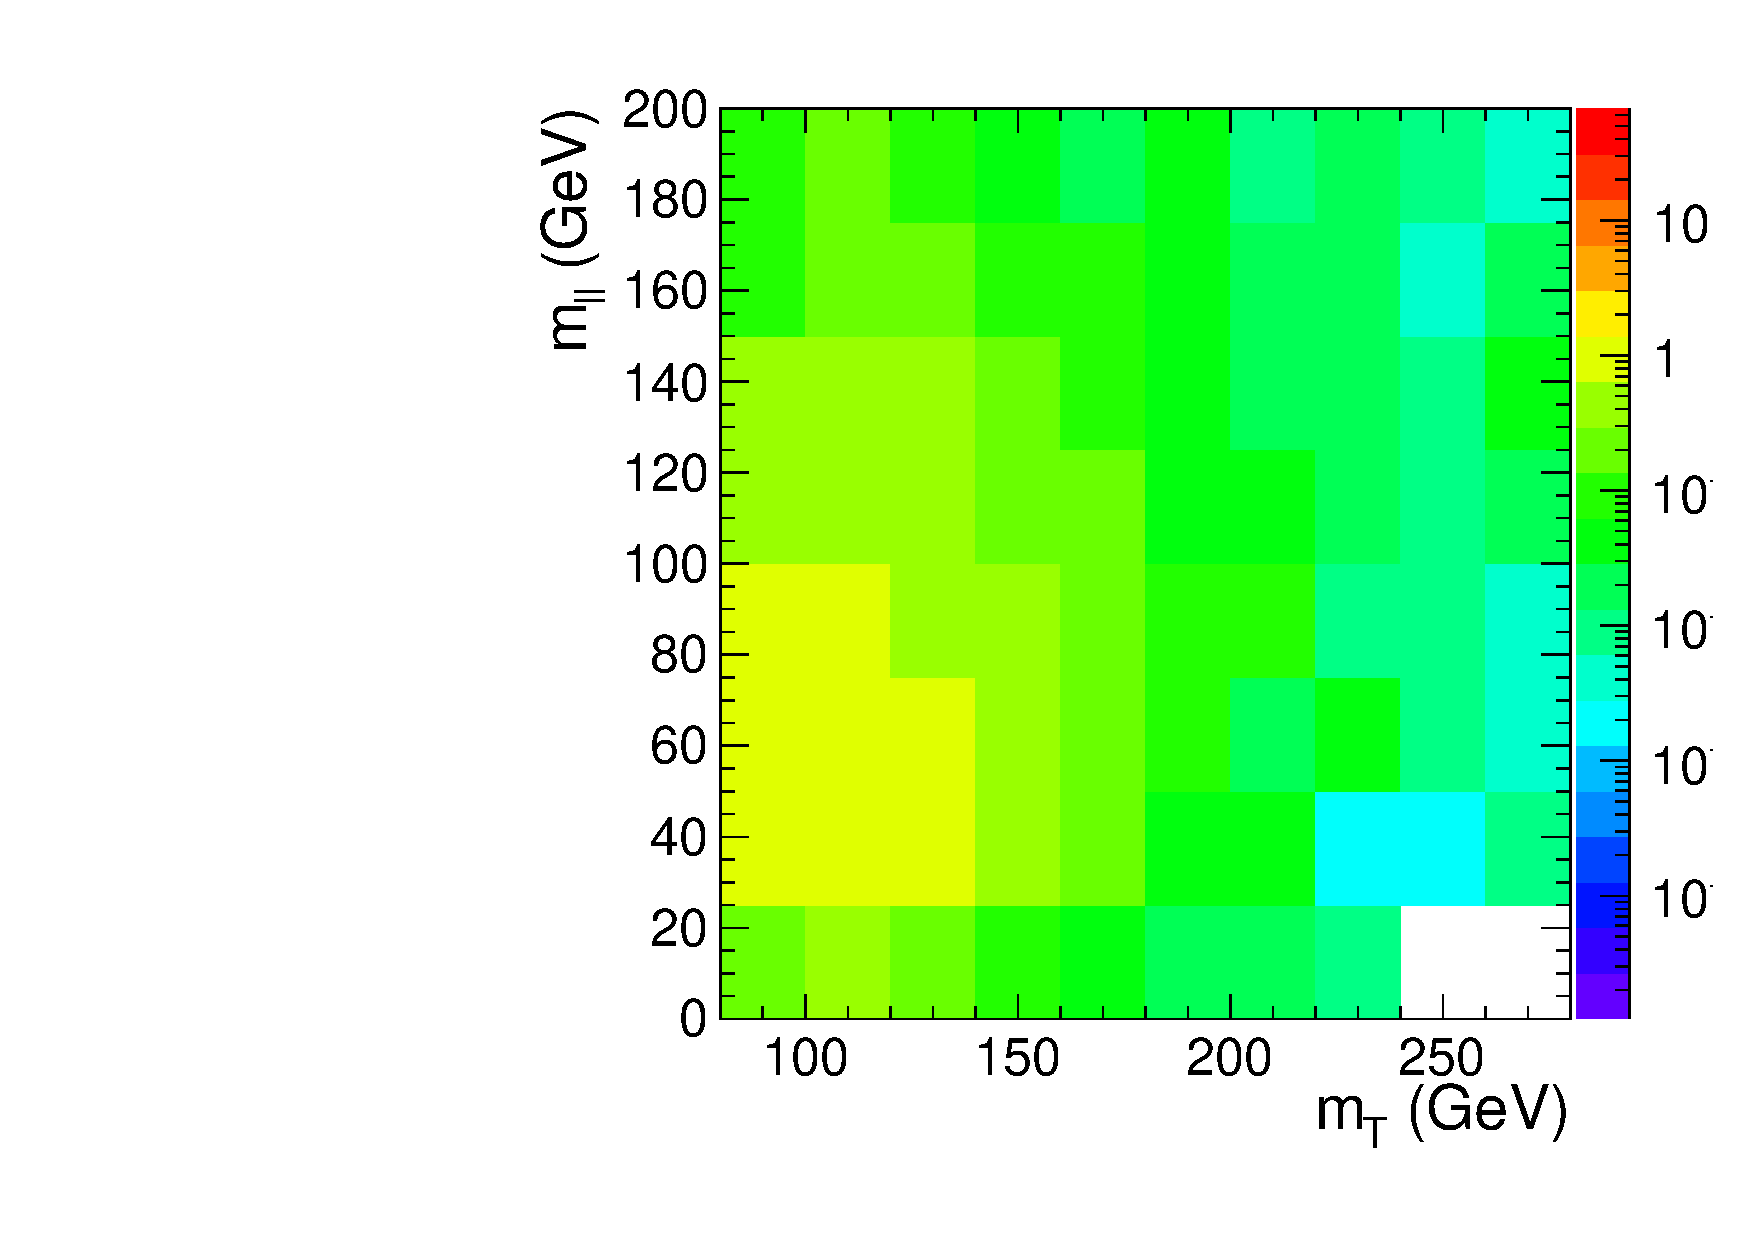
\includegraphics[width=.35\textwidth]{figures/templates/VV_2D_mH125_0j_of.pdf}
	}
	\subfigure[VV statistical uncertainty]{
	\centering
	\label{subfig:template_VVerr_125}
		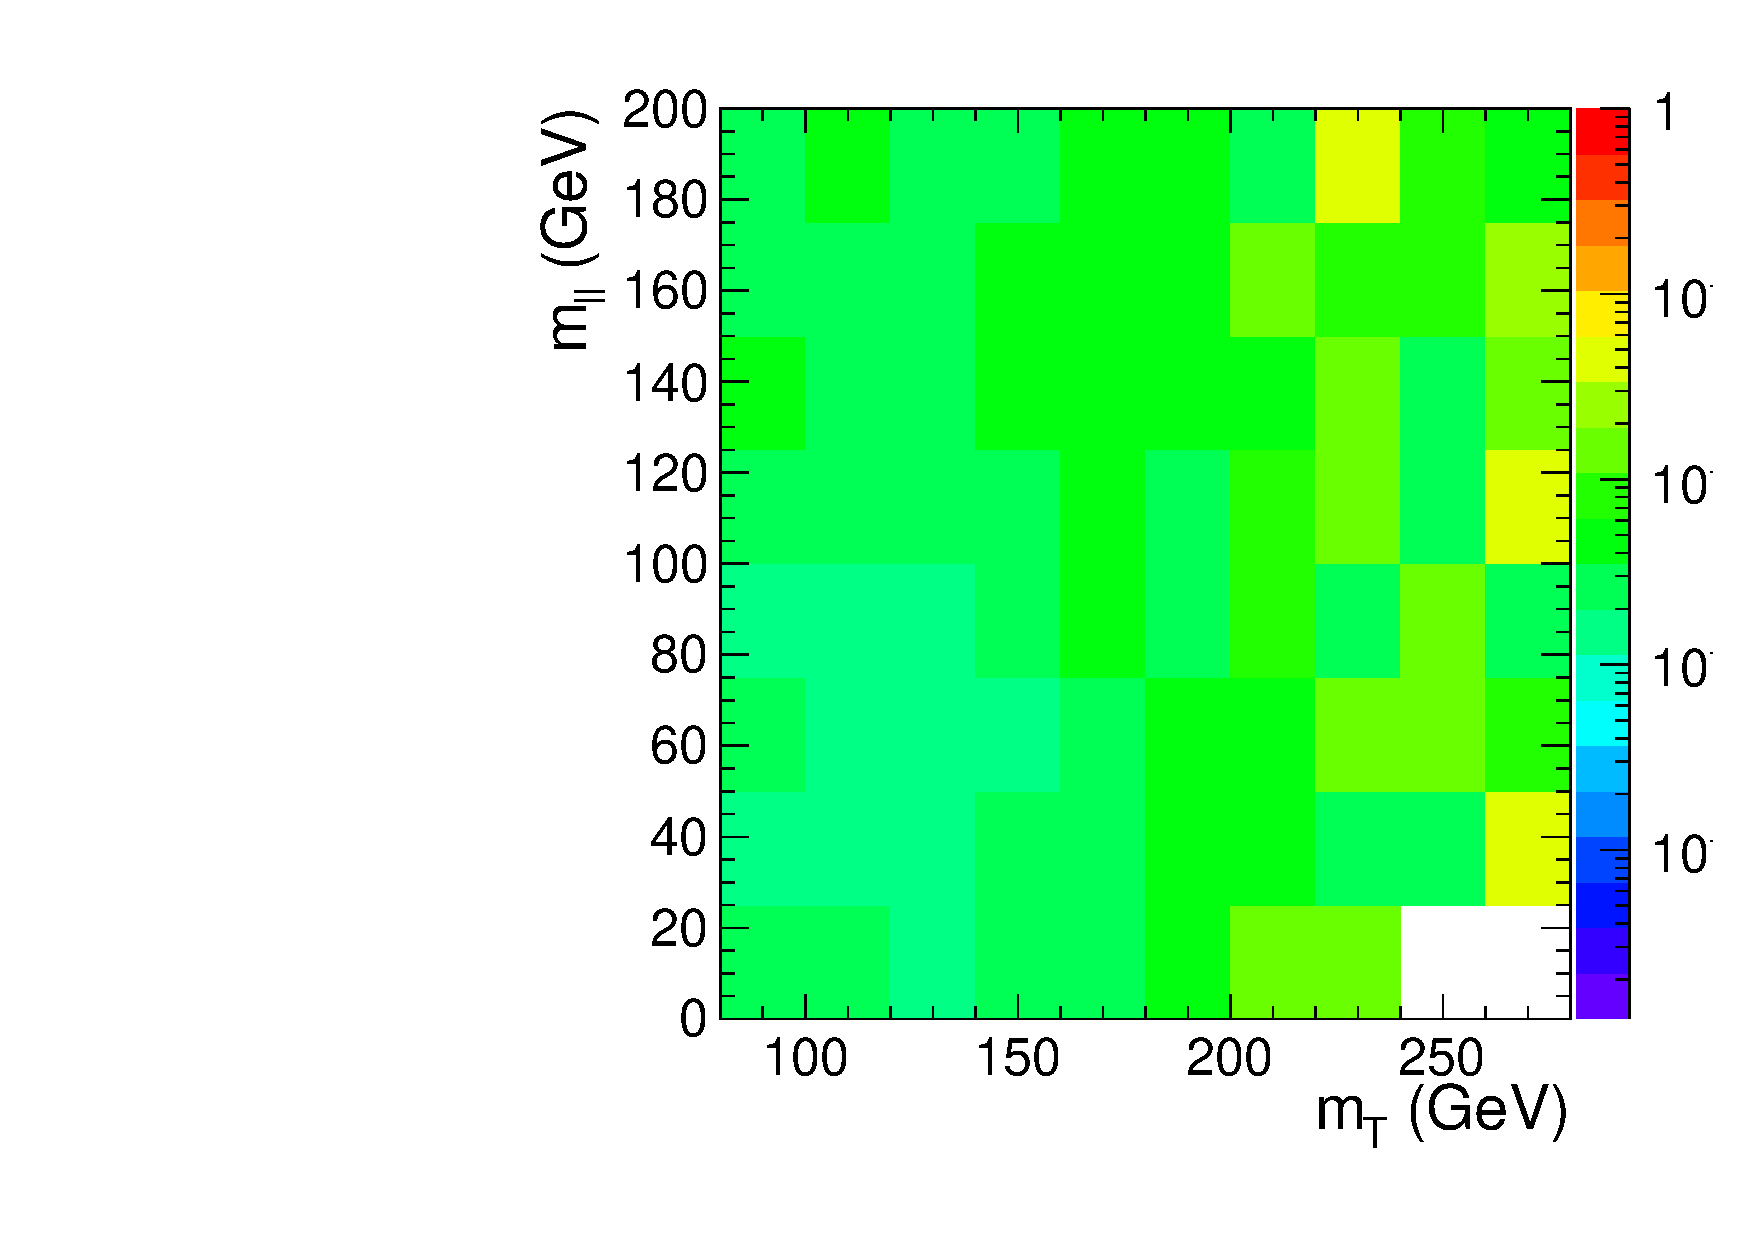
\includegraphics[width=.35\textwidth]{figures/templates/VVerr_2D_mH125_0j_of.pdf}
	}

	\caption{2D templates at \mHi = 125 \GeV} 
	\label{fig:templates_125_2}

\end{figure}

\begin{figure}[!hbtp]
	
	%
	\centering
	\subfigure[Zjets]{
	\centering
	\label{subfig:template_Zjets_125}
		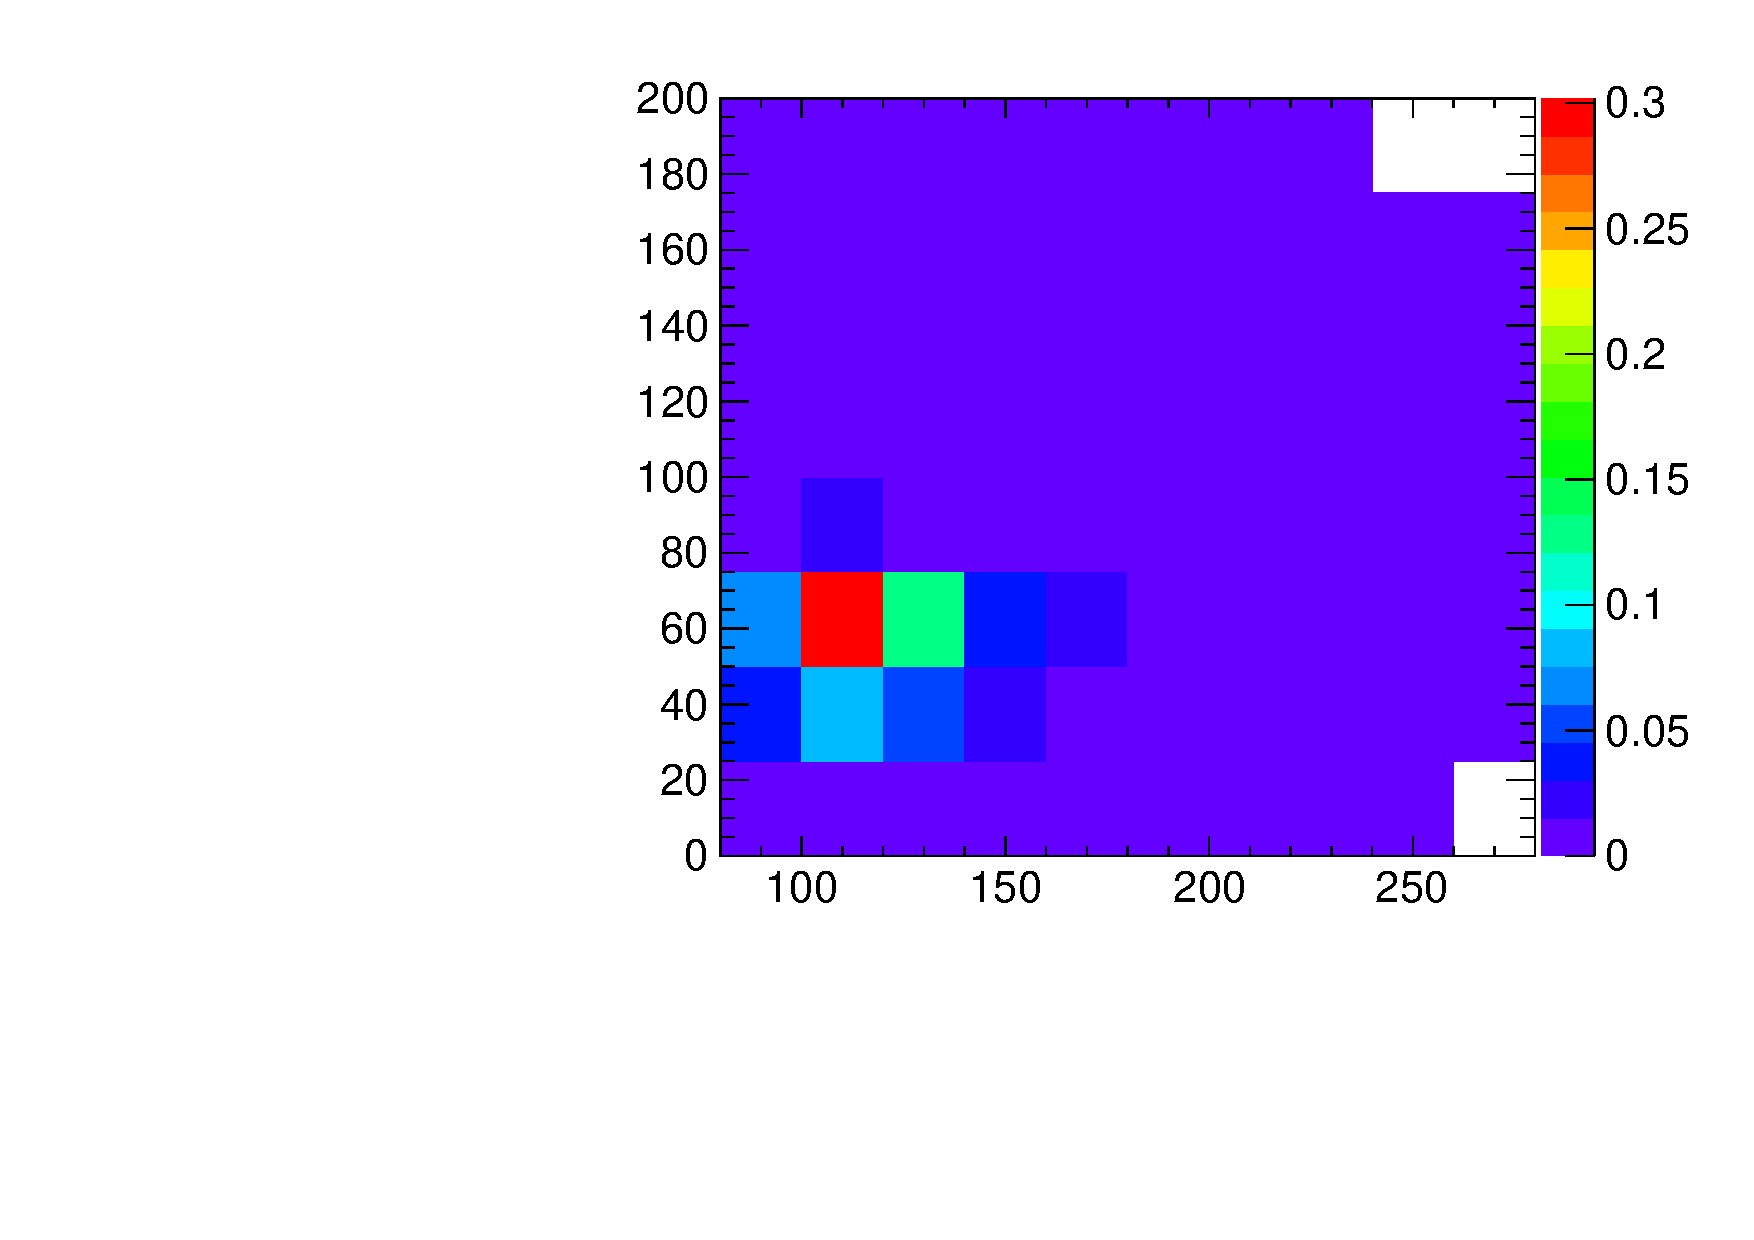
\includegraphics[width=.35\textwidth]{figures/templates/Zjets_2D_mH125_0j_of.pdf}
	}
	\subfigure[Zjets statistical uncertainty]{
	\centering
	\label{subfig:template_Zjetserr_125}
		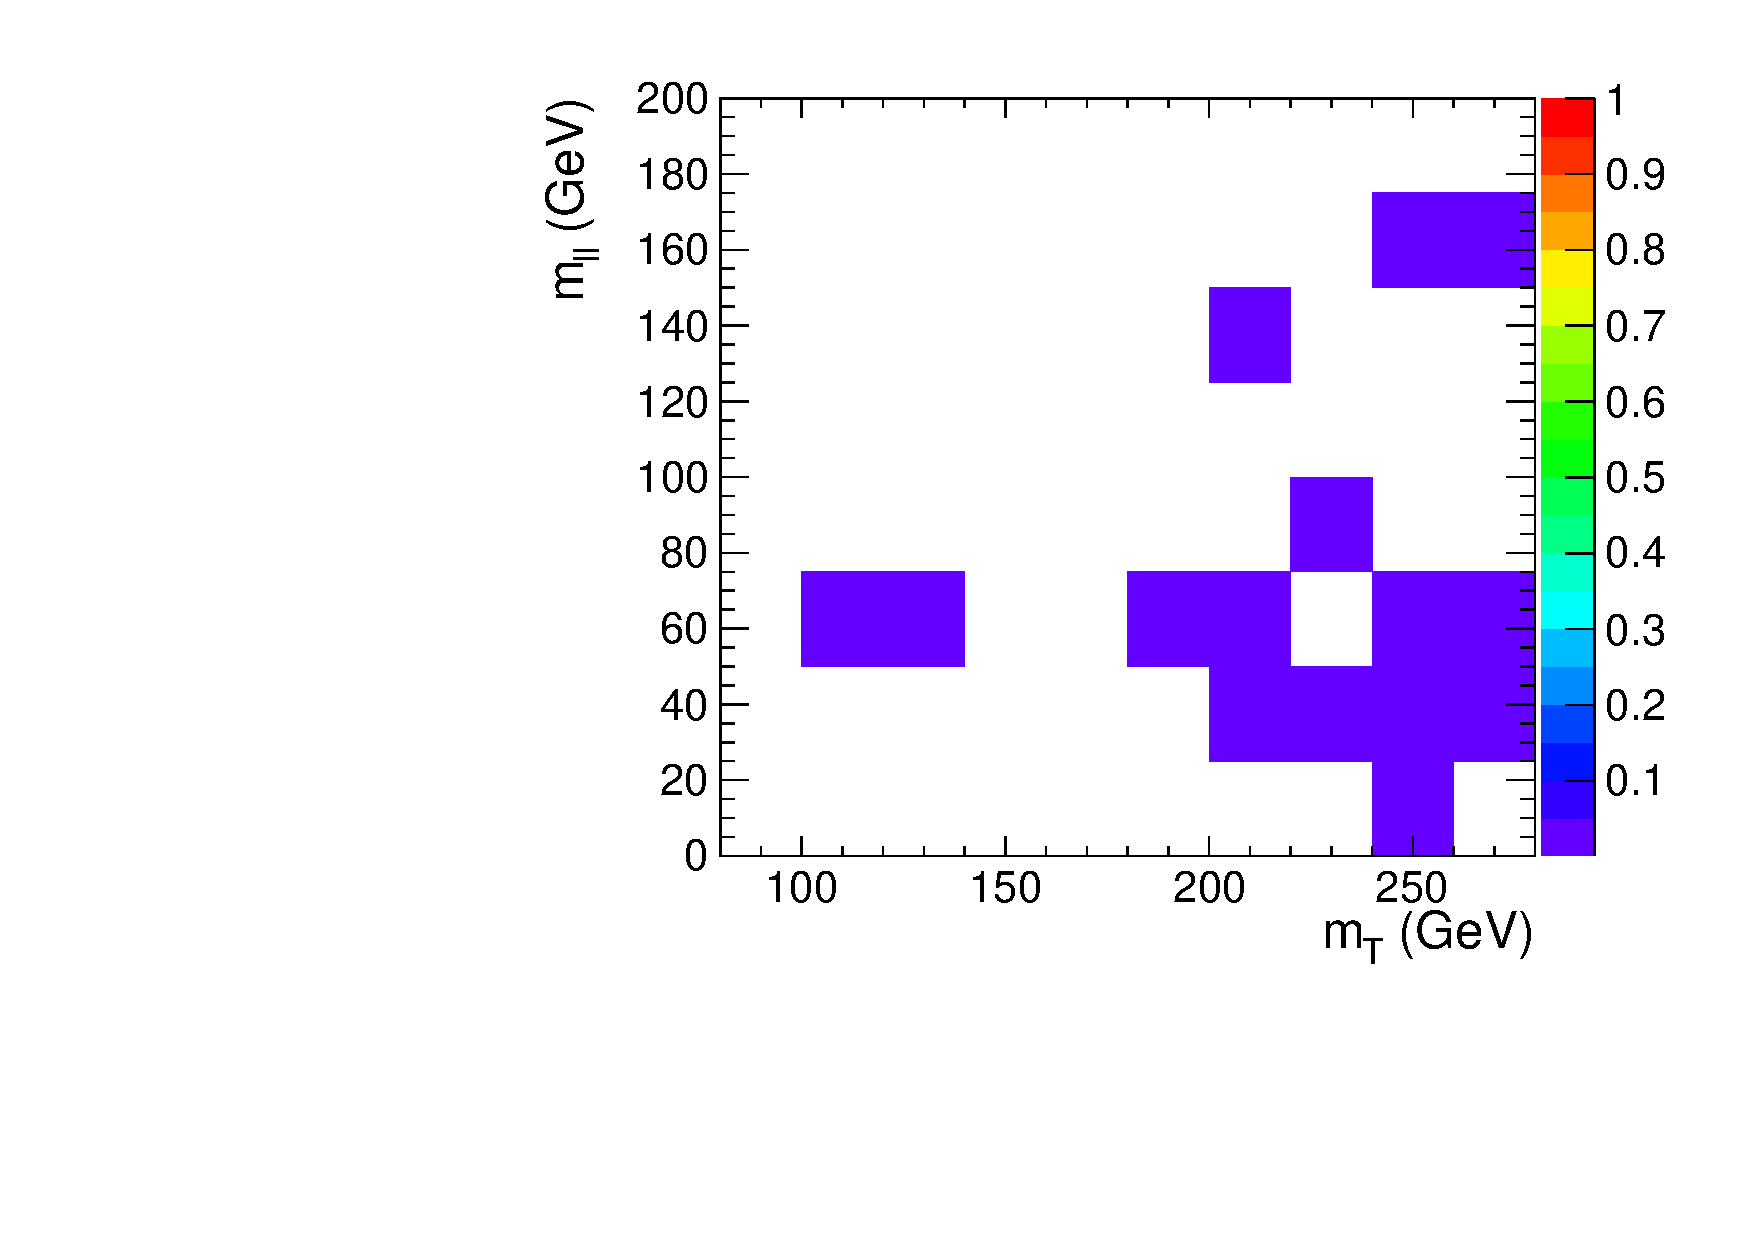
\includegraphics[width=.35\textwidth]{figures/templates/Zjetserr_2D_mH125_0j_of.pdf}
	}

	%
	\centering
	\subfigure[Wgamma]{
	\centering
	\label{subfig:template_Wgamma_125}
		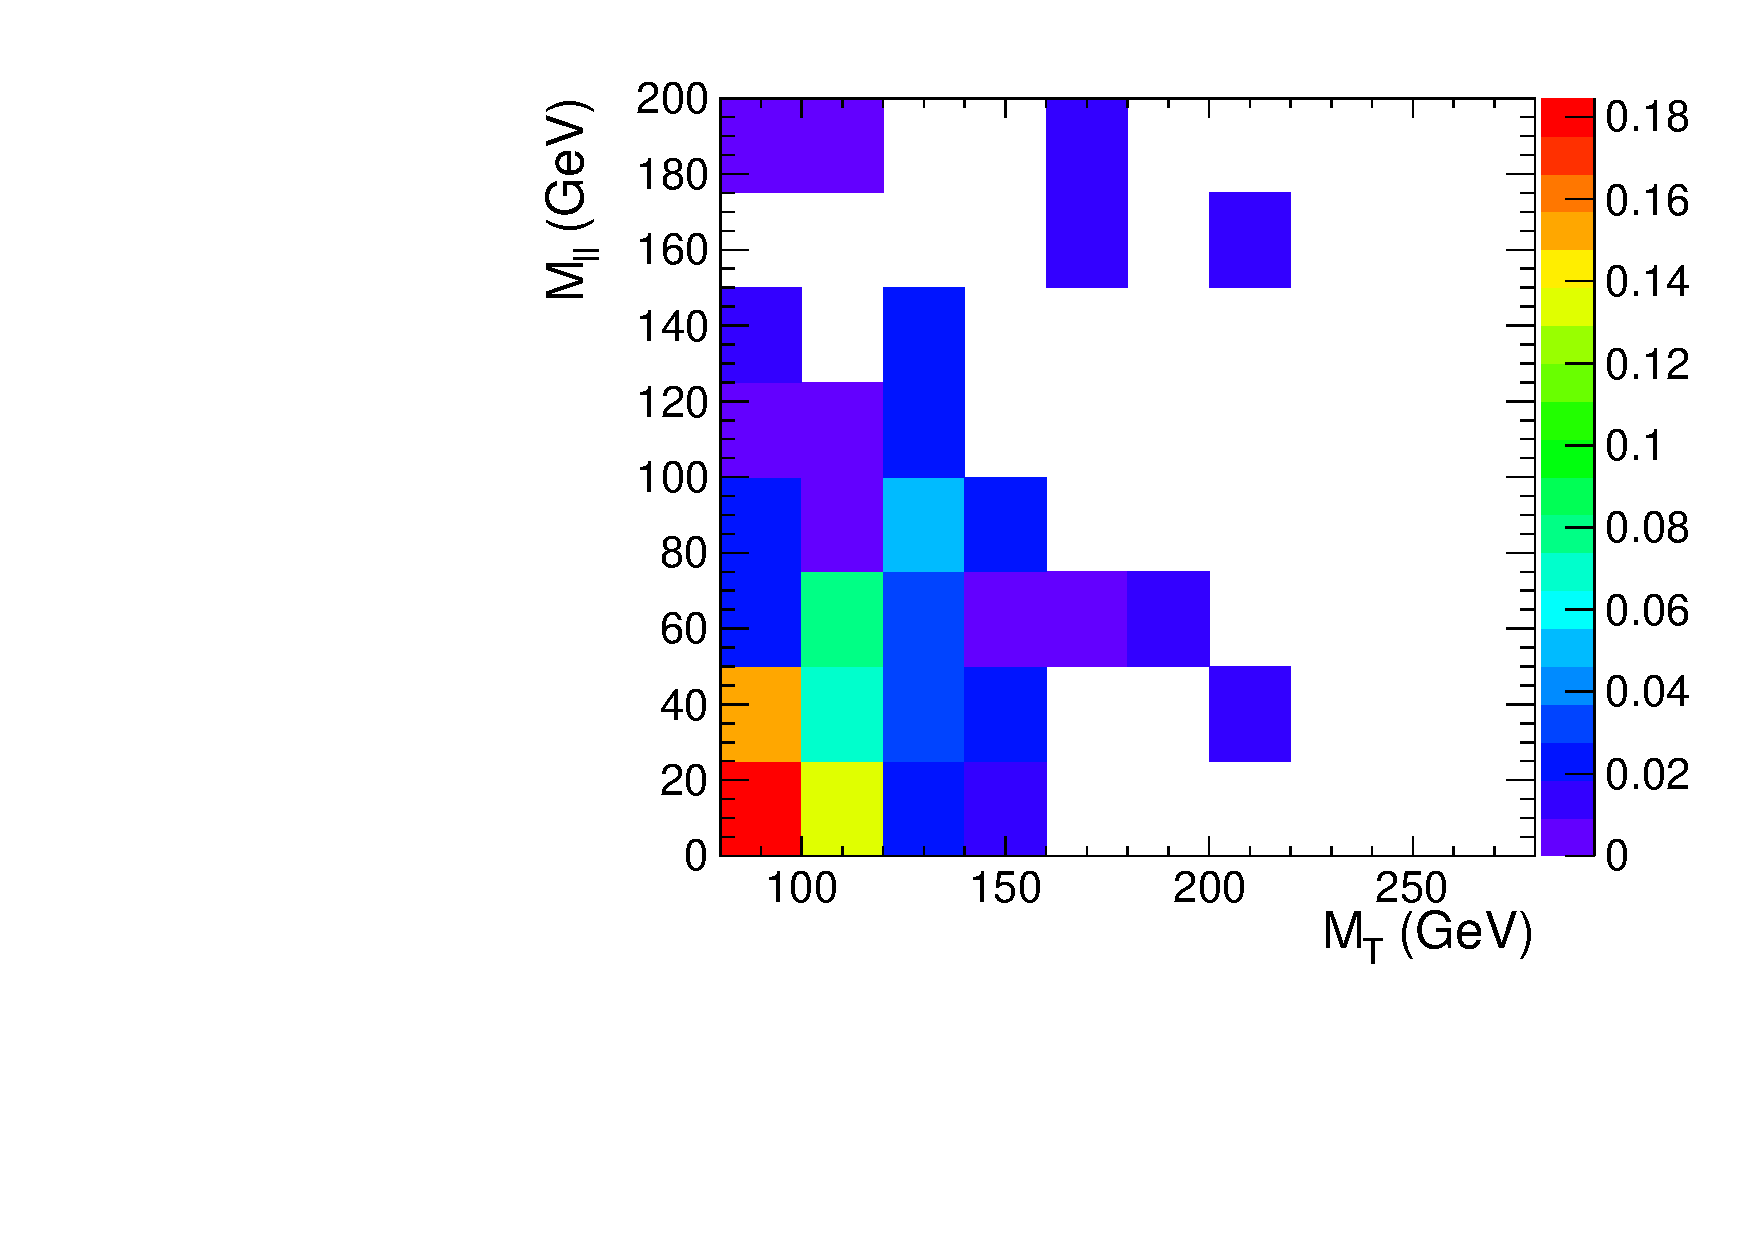
\includegraphics[width=.35\textwidth]{figures/templates/Wgamma_2D_mH125_0j_of.pdf}
	}
	\subfigure[Wgamma statistical uncertainty]{
	\centering
	\label{subfig:template_Wgammaerr_125}
		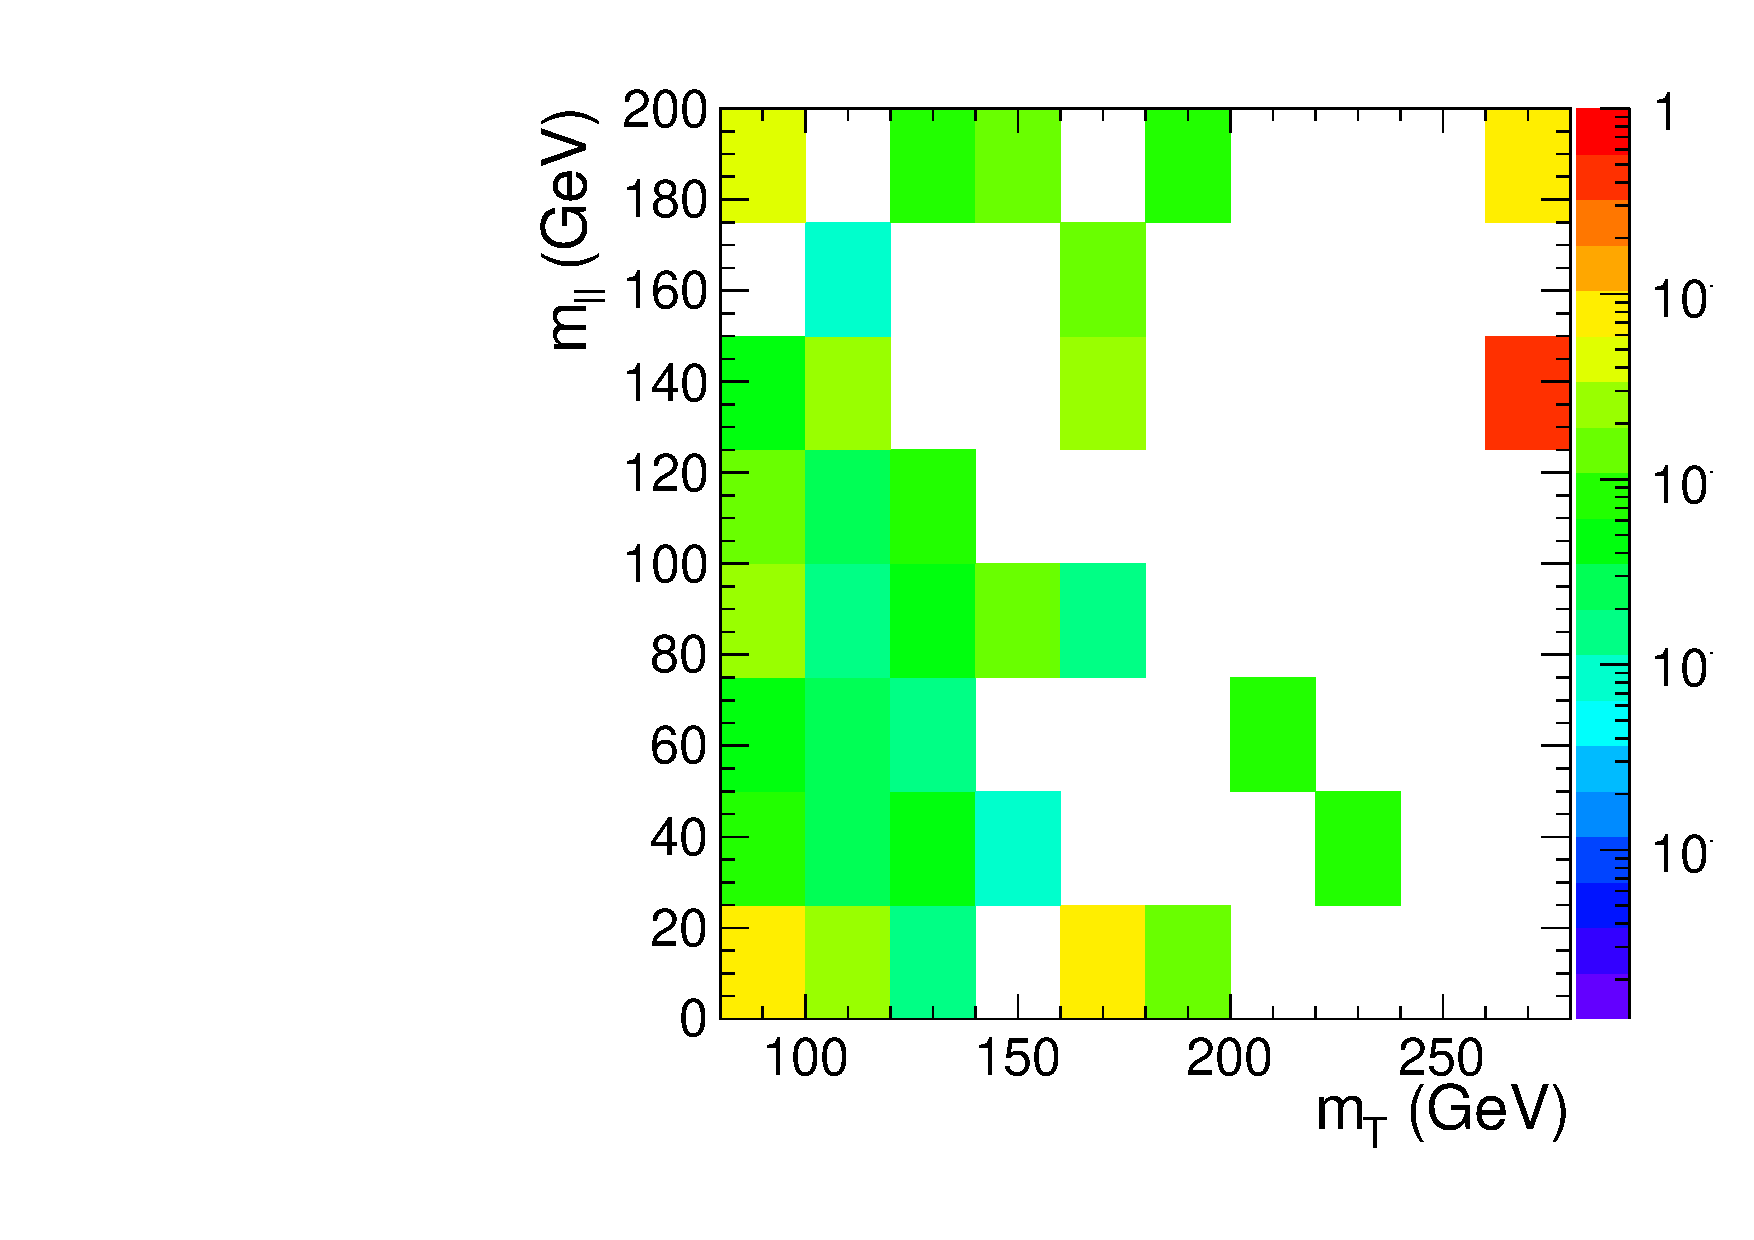
\includegraphics[width=.35\textwidth]{figures/templates/Wgammaerr_2D_mH125_0j_of.pdf}
	}

	\caption{2D templates at \mHi = 125 \GeV} 
	\label{fig:templates_125_3}

\end{figure} 

\begin{figure}[!hbtp]
	
	%
	\centering
	\subfigure[Stacked unrolled template linear]{
	\centering
	\label{subfig:template_unroll_stack_lin}
		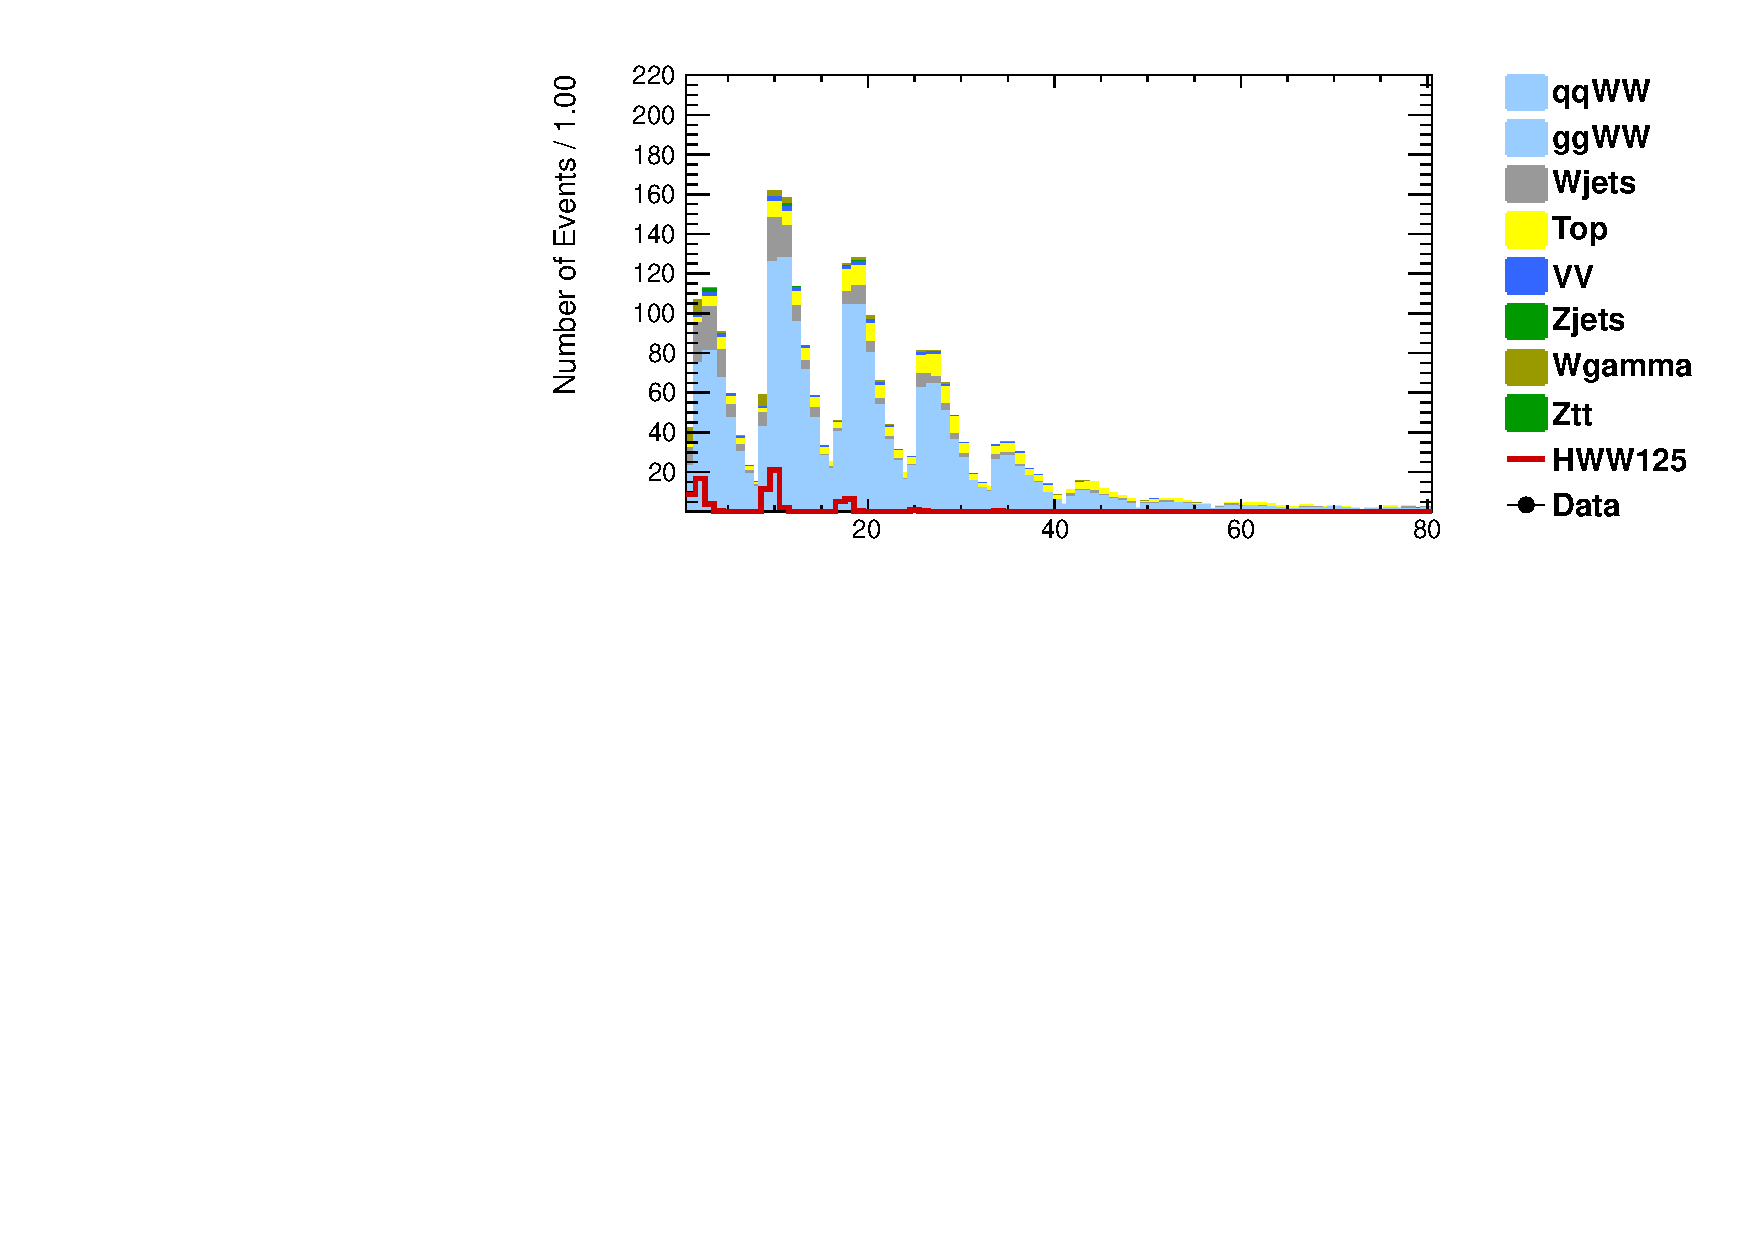
\includegraphics[width=.45\textwidth]{figures/templates/2D_mH125_0j_of_stack_lin.pdf}
	}
	\subfigure[Overlaid unrolled template linear]{
	\centering
	\label{subfig:template_unroll_overlay_lin}
		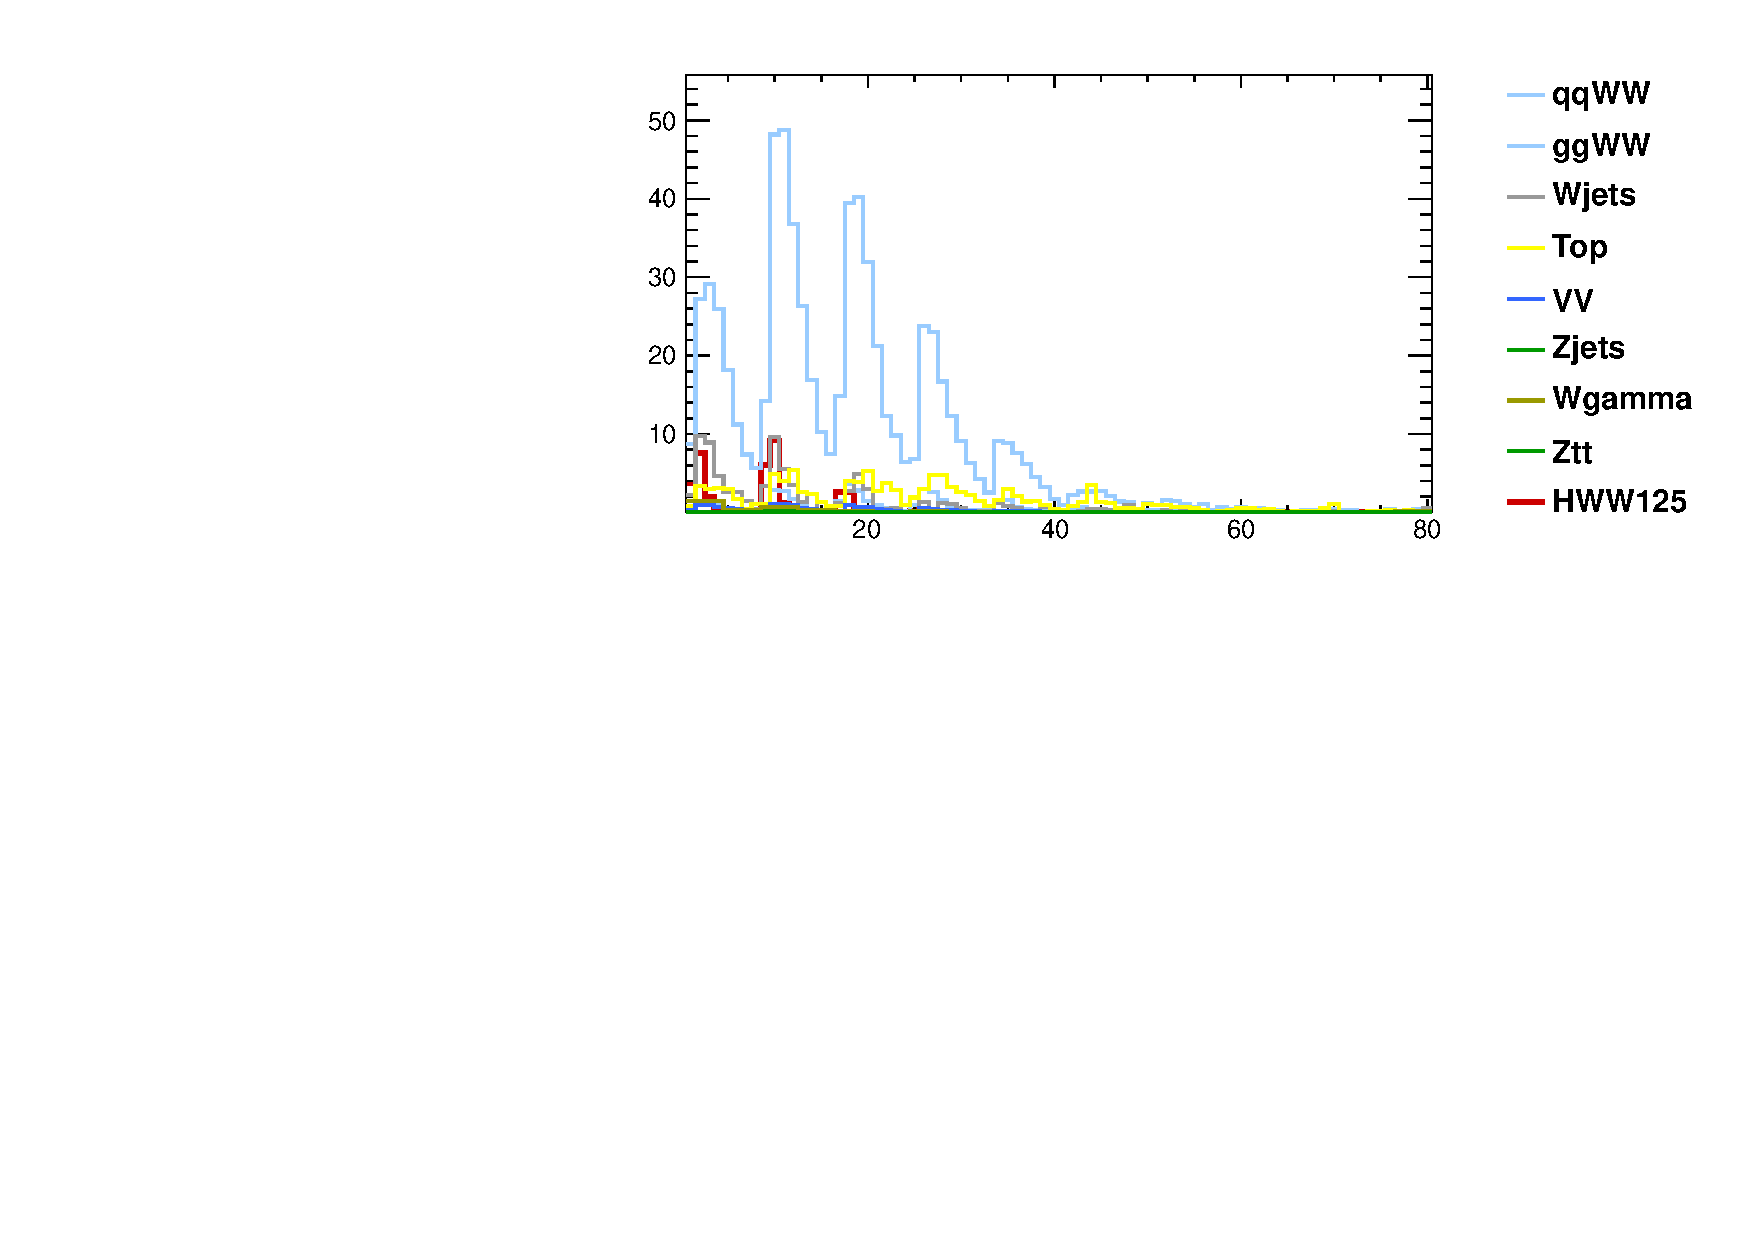
\includegraphics[width=.45\textwidth]{figures/templates/2D_mH125_0j_of_overlay_lin.pdf}
	}

	%
	\centering
	\subfigure[Stacked unrolled template in log scale]{
	\centering
	\label{subfig:template_unroll_stack_log}
		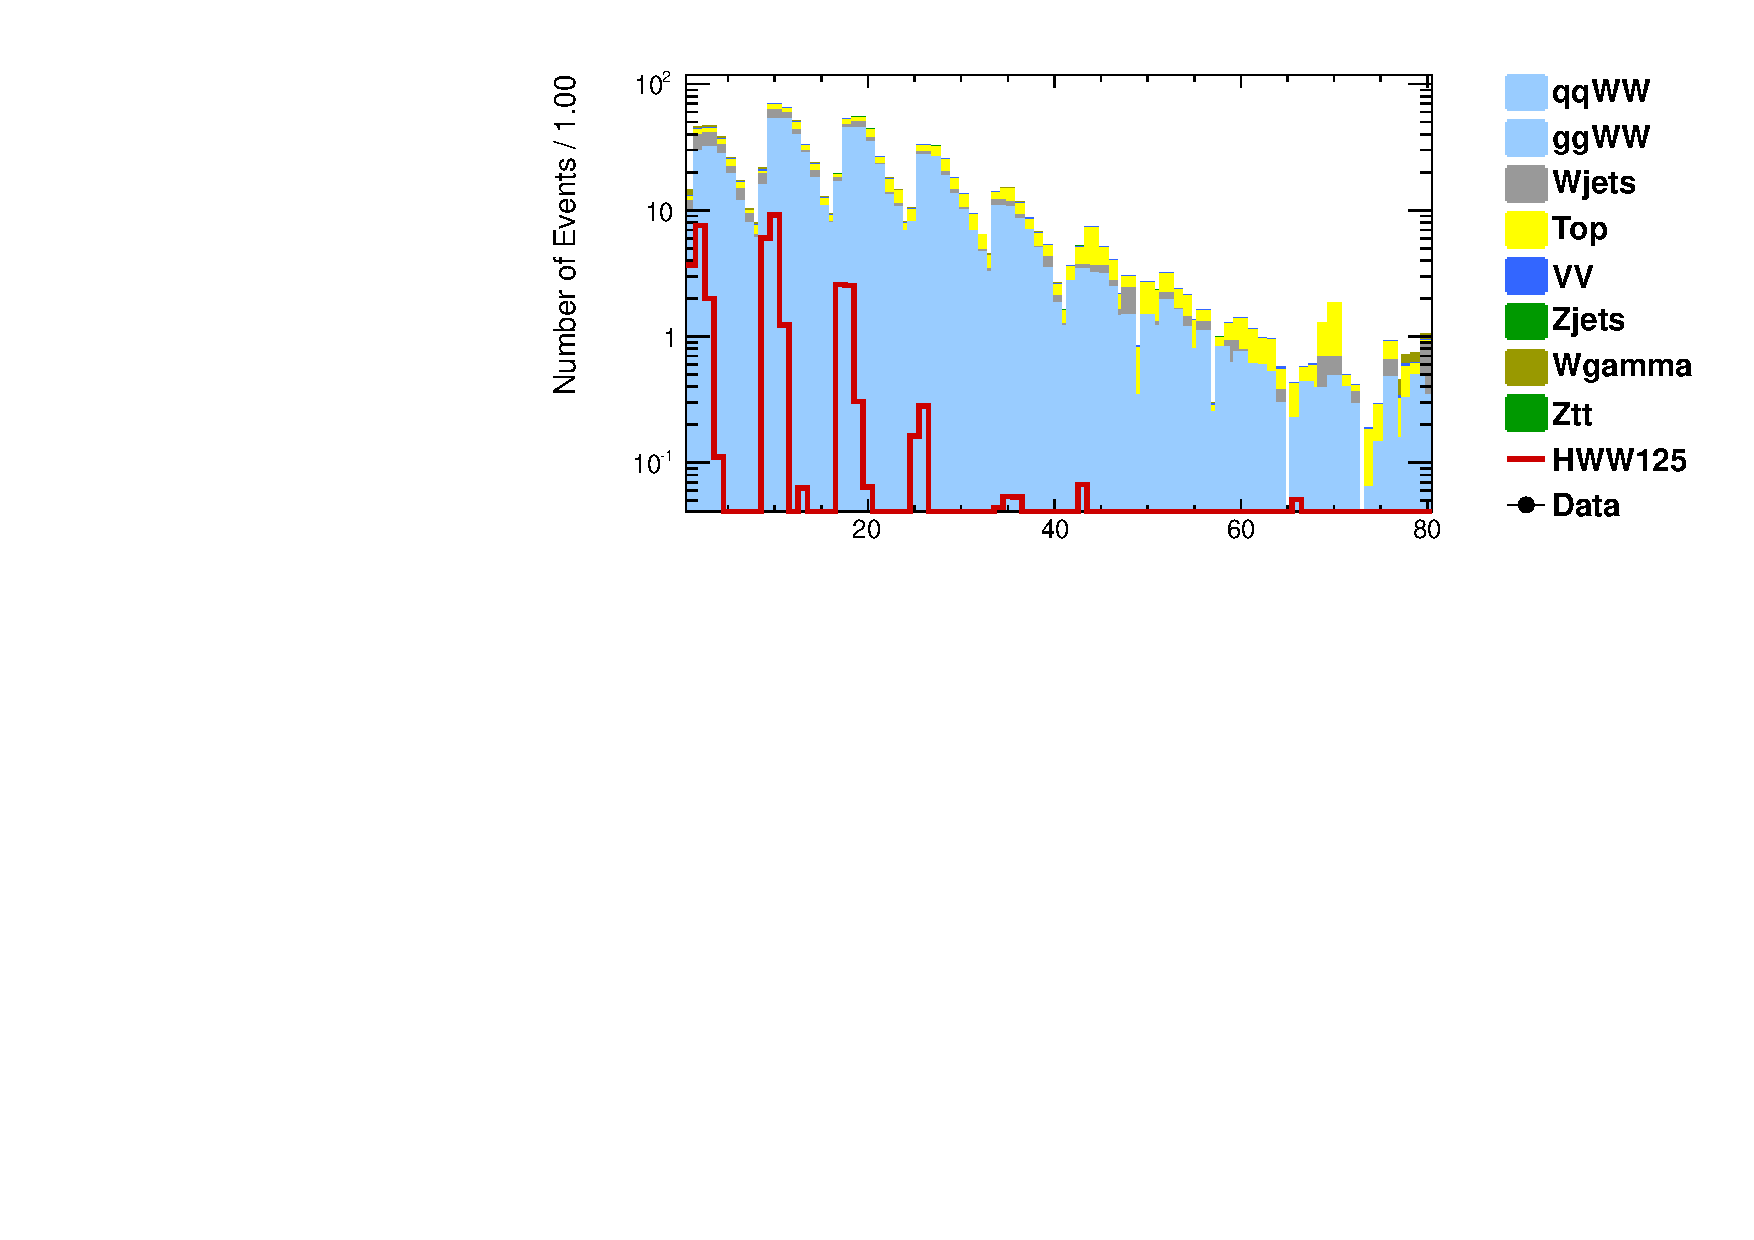
\includegraphics[width=.45\textwidth]{figures/templates/2D_mH125_0j_of_stack_log.pdf}
	}
	\subfigure[Overlaid unrolled template in log scale]{
	\centering
	\label{subfig:template_unroll_overlay_log}
		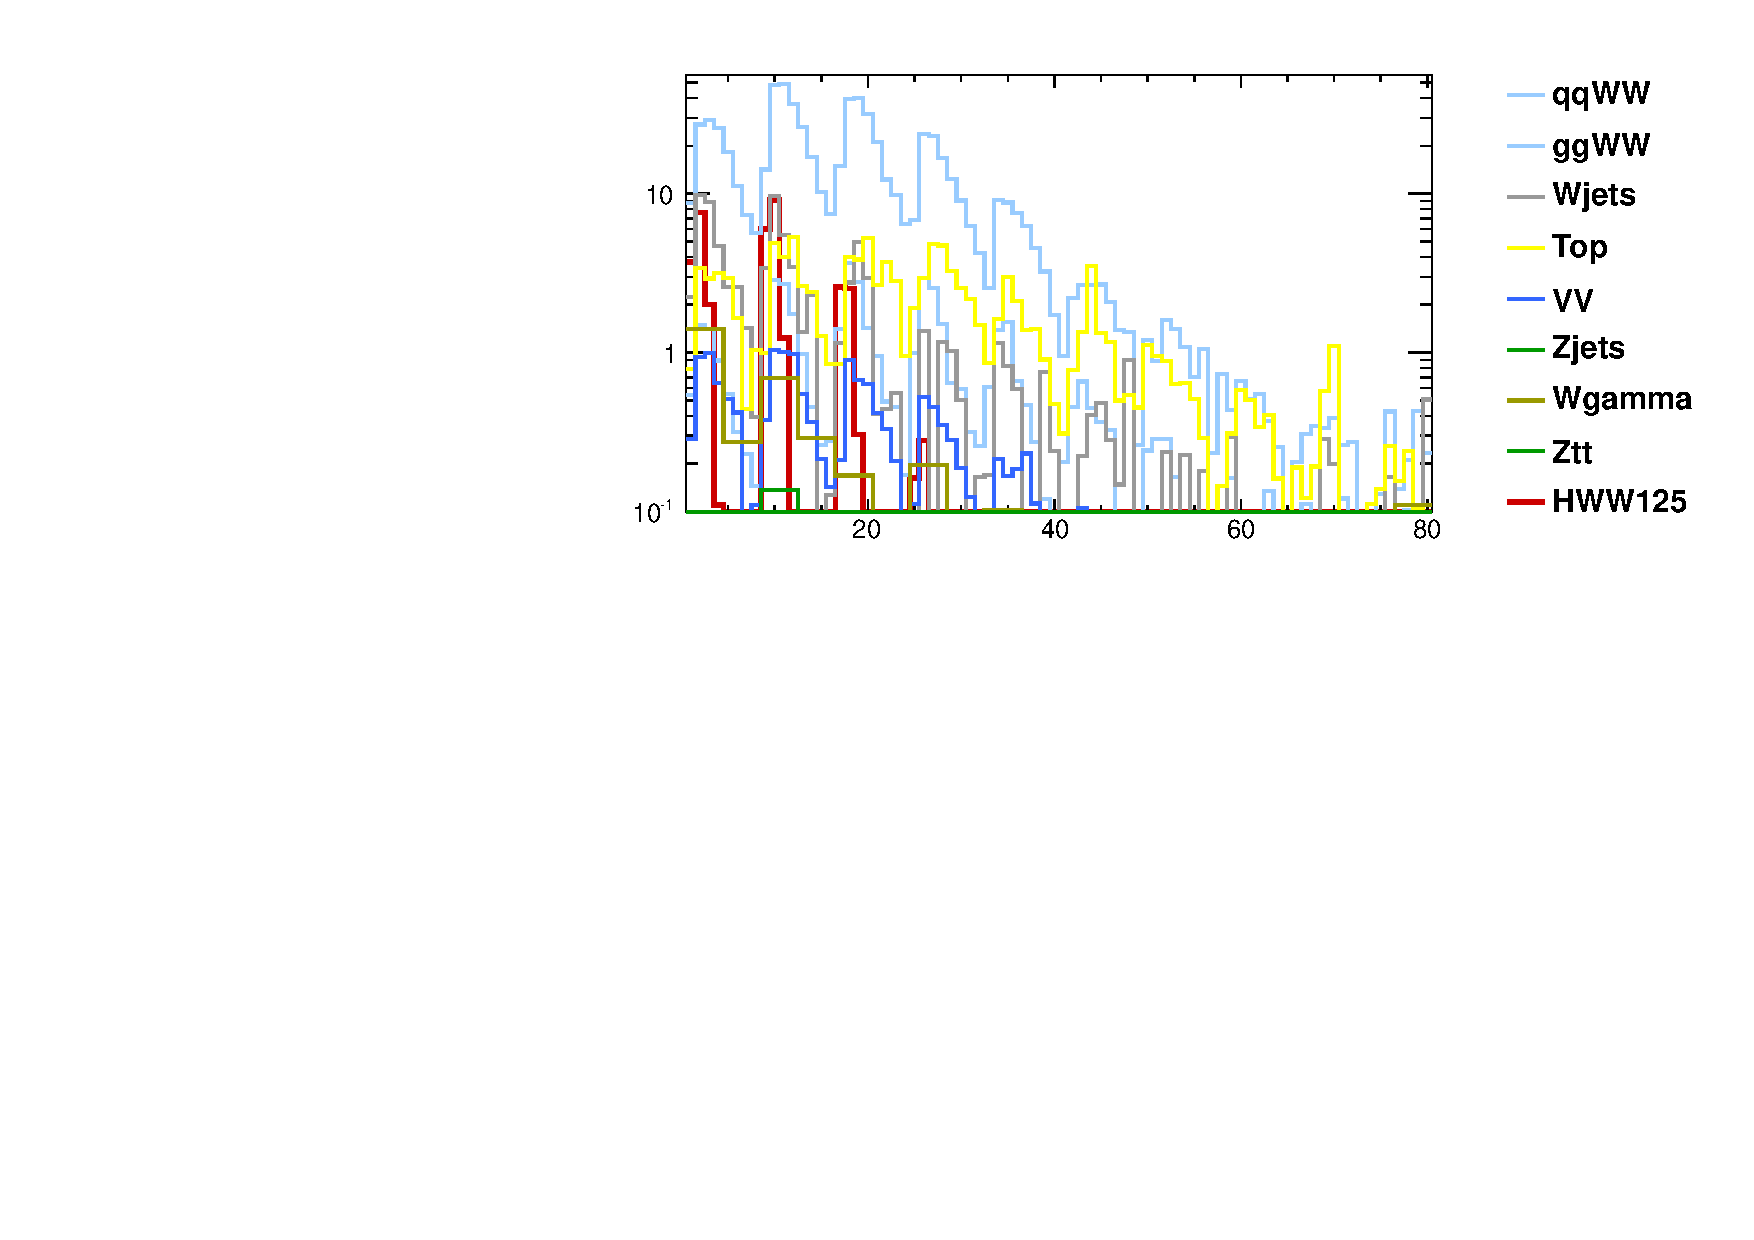
\includegraphics[width=.45\textwidth]{figures/templates/2D_mH125_0j_of_overlay_log.pdf}
	}

	\caption{Unrolled templates at \mHi = 125 \GeV} 
	\label{fig:templates_125_unroll}

\end{figure} 


Figures \ref{fig:templates_125_1} - \ref{fig:templates_125_3} show 2D templates(left) and 
its statistical uncertainties(right) at \mHi = 125 \GeV. The statistical uncertainties 
are relative to the total background yields. Templates for \mHi = 160 \GeV~and 200 \GeV~
are shown in appendix ~\ref{app:templates_160_200}.

  
  \subsection{Shape Uncertainties}
  \label{sec:shape_uncert}
  For the shape variation, we use the same technique used by BDT shape analysis \cite{MVASyst}.


%
\newpage
\section{Performance}
  \label{sec:performance}
  To compare the performance of the BDT shape analysis and the 2D method,
we calculate expected significance using the standard Combination tool \cite{combine}. 
The comparison is performed for the the 0 and 1-jet categories, as well
as their combination with the VBF category. 
In all cases only the different lepton flavor
final state is considered.


  
  \subsection{Expected Significance at \intlumiEightTeV }
  \label{sec:exp_significance_5fb}
  Table~\ref{tab:exp_sig_0j}, \ref{tab:exp_sig_1j}, and \ref{tab:exp_sig_01j} 
show expected signicances in 0jet, 1jet, and 0+1jet bins, respectively.
They improve by about 20 \% at low mass and 
and are degraded as mass increases. 
At \mHi = 125 \GeV~improvement is 24 \% with 0 and 1 jets combined.

\begin{table}[!htb] 
	\centering
	\begin{tabular}{c | c c | c }
   	\hline \hline
	\mHi & BDT & 2D & Improvement(\%) \\
	\hline
	110	& 0.36 & 0.36 & 0	\\
	115	& 0.62 & 0.69 & 12	\\
	120	& 0.94 & 1.15 & 23 	\\
	125	& 1.39 & 1.83 & 32 	\\
	130	& 1.91 & 2.44 & 28 	\\
	135	& 2.50 & 3.23 & 29 	\\
	140	& 3.26 & 3.82 & 17 	\\
	150	& 4.98 & 5.59 & 12 	\\
	160	& 7.17 & 8.43 & 18 	\\
	170	& 6.22 & 7.73 & 24 	\\
	180	& 5.46 & 5.82 & 7 	\\
	190	& 3.44 & 3.73 & 9 	\\
	200	& 2.89 & 2.90 & 1 	\\
	250	& 1.97 & 1.84 & -6 	\\
   	\hline \hline
	\end{tabular}
	\label{tab:exp_sig_0j}
	\caption{Expected significances in 0 jet bin for BDT and 2D methods}
\end{table}


\begin{table}[!htb] 
	\centering
	\begin{tabular}{c | c c | c }
   	\hline \hline
	\mHi & BDT & 2D & Improvement(\%) \\
	\hline
	110 & 0.21 & 0.26 & 24	\\
	115 & 0.38 & 0.47 & 21	\\
	120 & 0.66 & 0.80 & 21	\\
	125 & 1.01 & 1.19 & 18	\\
	130 & 1.41 & 1.65 & 16	\\
	135 & 1.73 & 2.18 & 26	\\
	140 & 2.45 & 2.65 & 8	\\
	150 & 3.76 & 3.75 & 0	\\
	160 & 6.17 & 5.69 & -8	\\
	170 & 5.71 & 4.96 & -13	\\
	180 & 3.74 & 3.77 & 1	\\
	190 & 2.68 & 2.52 & -6	\\
	200 & 2.11 & 2.01 & -5	\\
	250 & 1.37 & 1.22 & -11	\\
   	\hline \hline
	\end{tabular}
	\label{tab:exp_sig_1j}
	\caption{Expected significances in 1 jet bin for BDT and 2D methods}
\end{table}
  
\begin{table}[!htb] 
	\centering
	\begin{tabular}{c | c c | c }
   	\hline \hline
	\mHi & BDT & 2D & Improvement(\%) \\
	\hline
	110 & 0.40 & 0.44 & 10	\\
	115 & 0.70 & 0.83 & 18	\\
	120 & 1.09 & 1.39 & 28	\\
	125 & 1.64 & 2.15 & 30	\\
	130 & 2.23 & 2.90 & 30	\\
	135 & 2.88 & 3.82 & 33	\\
	140 & 3.89 & 4.54 & 17	\\
	150 & 6.17 & 6.60 & 7	\\
	160 & 9.90 & 10.02 & 1	\\
	170 & 8.94 & 9.04 & 1	\\
	180 & 6.72 & 6.81 & 1	\\
	190 & 4.45 & 4.44 & 0	\\
	200 & 3.69 & 3.50 & -5	\\
	250 & 2.40 & 2.22 & -8	\\
   	\hline \hline
	\end{tabular}
	\label{tab:exp_sig_01j}
	\caption{Expected significances in 0+1 jet bins for BDT and 2D methods}
\end{table} 

Now, we observe 25 \% improvement with respect to BDT analysis at \mHi = 125 \GeV. 
Because we use difference bin size and  $[\mt,\mll]$ ranges,
we test the effect of them to the performance.  
Table~\ref{tab:exp_sig_understand} shows expected significance 
with different bin size (top) and different ranges (bottom).
For testing bin size, the range is kept same and for testing 
ranges, bin size is kept same.  
The expected significance changes by less than 10 \% 
by increasing number of bins by factor 4, from 4 to 16
and it is comparable with BDT analysis which gives 1.80.
On the other hand, by extending ranges expected significance 
increases by 20 \% from BDT region to larger $[\mt,\mll]$ region.    

\begin{table}[!htb] 
	\centering
	\begin{tabular}{ccc }
   	\hline \hline
 	\multicolumn{3}{c}{Same range and different bin size}  						\\ 
	\hline
	Binning ($\mt \times \mll $) & Range & expected significance 				\\ 
   	\hline \hline
	\multirow{2}{*}{$2 \times 2$} 	& $80 < \mt < 125$	& \multirow{2}{*}{1.71} \\ 
									& $12 < \mll < 80$	& 						\\ 
	\hline
	\multirow{2}{*}{$3 \times 3$} 	& $80 < \mt < 125$	& \multirow{2}{*}{1.69} \\ 
									& $12 < \mll < 80$	& 						\\ 
	\hline
	\multirow{2}{*}{$4 \times 4$} 	& $80 < \mt < 125$	& \multirow{2}{*}{1.75} \\ 
									& $12 < \mll < 80$	& 						\\ 
   	\hline \hline 
 	\multicolumn{3}{c}{}  														\\ 
   	\hline \hline 
 	\multicolumn{3}{c}{Different range and same bin size} 						\\
	\hline
	Binning ($\mt \times \mll $) 	& Range 			& expected significance \\
   	\hline \hline
	\multirow{2}{*}{$2 \times 4$}   & $80 < \mt < 120$  & \multirow{2}{*}{1.81}	\\
									& $0 < \mll < 100$  & 				   		\\
	\hline
	\multirow{2}{*}{$5 \times 4$}   & $80 < \mt < 180$  & \multirow{2}{*}{1.81}	\\
									& $0 < \mll < 100$  & 				   		\\
	\hline
	\multirow{2}{*}{$8 \times 6$}   & $80 < \mt < 240$  & \multirow{2}{*}{2.07}	\\
									& $0 < \mll < 150$  & 				   		\\
   	\hline \hline 
	\end{tabular}
	\label{tab:exp_sig_understand}
	\caption{Top table shows expected significance with the same range but different 
	bin sizes. Bottom table shows expected significance with the same bin size but different 
	ranges. Expected significance from BDT analysis is 1.64.}
\end{table} 

  
  \newpage
  \subsection{Expected Significance at 20~\ifb }
  \label{sec:exp_significance_20fb}
  For the projection to 20~\ifb, top normalization uncertainty is halved
because it is driven by data statistics. Table~\ref{tab:exp_sig_20fb} shows
that the expected significance in 20~\ifb~is 80-90 \% larger than that in 5~\ifb
at all mass points. This means that significance is scaled almost statistically.
At \mHi = 125 \GeV the expected  significance in 20~\ifb is 4$\sigma$.

\begin{table}[htb] 
	\centering
	\begin{tabular}{c | c c | c }
   	\hline \hline
	\mHi & 5.1~\ifb & 20~\ifb & Improvement(\%) \\
	\hline 
	110 & 0.46 & 0.85 & 85 \\
	115 & 0.86 & 1.58 & 83 \\
	120 & 1.44 & 2.62 & 82 \\
	125 & 2.22 & 4.01 & 80 \\
	130 & 3.02 & 5.41 & 79 \\
	135 & 4.04 & 7.34 & 82 \\
	140 & 4.78 & 8.74 & 83 \\
	150 & 6.13 & 11.66 & 90 \\
	160 & 9.86 & 18.35 & 86 \\
	170 & 8.45 & 15.44 & 83 \\
	180 & 5.98 & 11.11 & 86 \\
	190 & 3.88 & 7.20 & 85 \\
	200 & 3.14 & 5.79 & 85 \\
   	\hline \hline
	\end{tabular}
	\caption{Expected significances in 0+1 jet bins in 5.1~\ifb and 20~\ifb}
	\label{tab:exp_sig_20fb}
\end{table} 


%
\newpage
\section{Summary}
     \label{sec:summary}
     
We have performed a measurement of the $W^+W^-$ production cross-section
using an integrated luminosity of $\intlumi$ of $pp$ collision data at $\sqrt{s} = $
7~$\TeV$. The measurement was performed in the \wwlnln{} final state.
The $W^+W^-$ production cross-section was measured to be:

\begin{equation*}
\sigma_{WW}  = 53.95 \pm 2.05~\mathrm{(stat.)} \pm 4.30~\mathrm{(syst.)} \pm 2.43~\mathrm{(lumi.)~pb},
\end{equation*}

to be compared with the standard model prediction \cite{Campbell:2011bn}:

\begin{equation*}
\sigma_{WW}  = 47 \pm 2 ~\mathrm{pb}.
\end{equation*}




%===================================================================================================
\clearpage

\vspace*{-0.2cm}
\thebibliography{12}

\bibitem{pdg}
 K. Nakamura et al. (Particle Data Group), "Review of particle physics", J. Phys.G37 , 2010.

\bibitem{Higgs1}
F. Englert and R. Brout, "Broken symmetries and the masses of gauge bosons", Phys. Rev. Lett. 13,  1964.

\bibitem{Higgs2}
P. W. Higgs, "Broken symmetry and the mass of gauge vector mesons", Phys. Rev. Lett. 13, 1964.

\bibitem{Higgs3}
Guralnik, G.S. and Hagen, C.R. and Kibble, T.W.B., "Global Conservation Laws and Massless Particles", 
Phys.Rev.Lett. 13, 1964.

\bibitem{dittmar}
M.~Dittmar and H.~K.~Dreiner, Phys.\ Rev.\  D {\bf 55} (1997) 167".

\bibitem{HWW2010}
CMS Collaboration, "Measurement of WW Production and Search for the Higgs Boson in 
pp Collisions at $\sqrt{s}$ = 7 TeV", arXiv:1102.5429

\bibitem{HWW2011AN}
L.~Bauerdick et al, "A Higgs Boson Search in the Fully Leptonic $W^+W^-$ Final State", CMS AN-2011/155

\bibitem{VBTFCrossSectionNote}
J. Alcaraz Maestre, \textit{et al.}, "Updated Measurements of Inclusive W and Z Cross Sections 
at $\sqrt{s}=7$ TeV", CMS AN-2010/264.

\bibitem{ggWWError}
F.~ Stoeckli, "http://indico.cern.ch/getFile.py/access?contribId=0\&resId=1\&materialId=slides\&confId=49009", 
EWK Diboson meeting of March 12 2009.

\bibitem{json}
{\small
/afs/cern.ch/cms/CAF/CMSCOMM/COMM\_DQM/certification/Collisions11/7TeV/Prompt/Cert\_160404-163869\_7TeV\_PromptReco\_Collisions11\_JSON.txt
}

\bibitem{ElIso}
A. Vartak, M. LeBourgeois, V. Sharma, "Lepton Isolation in the CMS Tracker, ECAL and HCAL", CMS AN-2010/106.

\bibitem{PVDA}
W. Erdmann, M. LeBourgeois, B. Mangano, 
https://indico.cern.ch/getFile.py/access?contribId=5\&sessionId=3\&resId=1\&materialId=slides\&confId=127127, 
note in preparation.

\bibitem{NExpHits}
B. Mangano \textit{et al.}, "Improvement in Photon Conversion Rejection Performance Using 
Advanced Tracking Tools", AN-10-283.

\bibitem{fakeLeptonNote1}
S.~Xie, \textit{et al.}", "Study of Data-Driven Methods for Estimation of Fake Lepton Backgrounds", 
CMS AN-2009/120.

\bibitem{fakeLeptonNote2}
W.~Andrews, \textit{et al.}, "Fake Rates for dilepton Analyses", CMS AN-2010/257.

\bibitem{fakeLeptonBkgSpillage1}
 F. Golf, D. Evans, J. Mulmenstadt  \textit{et al.}, ``Expectations for observation of top quark pair production in the dilepton final state with the early CMS data'', CMS AN-2009/050.

\bibitem{dyestnote}
W. Andrews, et al., “A Method to Measure the Contribution of $\dyll$ to a di-lepton+ MET Selection”, CMS AN-2009/023 (2009).

\bibitem{jes}
CMS Collaboration, "Jet Energy Calibration with Photon+Jet Events", PAS JME-09-004.

\bibitem{jetpas}
CMS Collaboration, "Jet Performance in pp Collisions at $\sqrt{s}=7 \rm\ TeV$", PAS JME-10-003.

\bibitem{btag}
CMS collaboration, "Commissioning of b-jet identification with pp collisions at $\sqrt{s}=7~\TeV$, BTV-10-001.

\bibitem{antikt}
Cacciari, Matteo and Salam, Gavin P. and Soyez, Gregory, "The anti-$k_t$ jet clustering 
algorithm", JHEP 04,  2008.

\bibitem{ConversionNote}
W.~Andrews, \textit{et al.}, "Study of photon conversion rejection at CMS", CMS AN-2009/159.

\bibitem{tmva}
A. Hoecker, \textit{et al.}, "TMVA - Toolkit for Multivariate Data Analysis", arXiv:physics/0703039, 2007.

\bibitem{XS}
CMS Generator group, Standard Model Cross Sections for CMS at 7 TeV, 2010.

\bibitem{PDF4LHC}
PDF4LHC Working Group, 
{\tt http://www.hep.ucl.ac.uk/pdf4lhc/PDF4LHCrecom.pdf}

\bibitem{Nadolsky:2008zw}
Nadolsky, Pavel M. and others, "Implications of CTEQ global analysis for 
collider observables", Phys. Rev. D78 2008.

\bibitem{Martin:2009iq}
Martin, A. D. and Stirling, W. J. and Thorne, R. S. and Watt, G., "Parton 
distributions for the LHC, Eur. Phys. J. C63 2009.

\bibitem{Ball:2010de}
Ball, Richard D. and others, "A first unbiased global NLO determination 
of parton distributions and their uncertainties", arXiv 1002.4407.

\bibitem{bayesian}
A. O'Hagan and J.J. Forster, "Bayesian Inference", Kendall's Advanced Theory of Statistics, 
Arnold, London, 2B, 2004.

\bibitem{ref:tagprobe_mit_w}
G. Bauer {\it et. al.}, "Lepton ef?iencies for the inclusive W cross section measurement with 36.1pb$^{-1}$", AN2011/097

\bibitem{ref:tagprobe_snt_top}
W. Andrews {\it et. al.}, "Uncertainties on the Lepton Selection Efficiency for t$t\bar{t}$ Cross Section Analysis", AN2010/274

\bibitem{LHCHiggsCrossSectionWorkingGroup:2011ti}
LHC Higgs Cross Section Working Group, "Handbook of LHC Higgs Cross Sections: 
Inclusive Observables", CERN-2011-002, 2011.

\bibitem{PFMET} 
CMS Collaboration, ``CMS MET Performance in Events Containing Electroweak Bosons from pp Collisions at $\sqrt{s}=7$ TeV'', CMS PAS JME-2010-005 (2010)


\bibitem{trkMET} 
Marco Zanetti, ``MET with PU in $\hww\to2\ell$'', https://indico.cern.ch/conferenceDisplay.py?confId=131580
Benjamin Hooberman, ``MET with PU in MC and First 2011 Data'', https://indico.cern.ch/contributionDisplay.py?contribId=5\&confId=132579. 


\bibitem{lands}
Mingshui Chen and Andrey Korytov, https://mschen.web.cern.ch/mschen/lands/

\bibitem{MCFMHiggsProduction}
J. Campbell, R.K. Ellis, G. Zanderighi, ``Next-to-Leading order Higgs + 2 jet production via gluon fusion.'', JHEP 0610:028 (2006), hep-ph/0608194

\bibitem{MCFMVVProduction}
J. Campbell, R.K. Ellis, C. Williams, ``Vector boson pair production at the LHC.'', arxiv:hep-ph/1105.0020.

\bibitem{MITHggNote} 
G. Bauer et al., ``Higgs Search in the pp $\rightarrow$ H $\rightarrow$ $\gamma\gamma$ channel at $\sqrt{s}=7$ TeV'', CMS AN-2011/168. 


%===================================================================================================

\clearpage 
\appendix
\appendixpage
  \section{Templates at \mHi = 160 \GeV~and 200 \GeV}
     \label{app:templates_160_200}
     In this appendix 2D templates at \mHi = 160 \GeV~and 200 \GeV~are shown.

%%%%%% mH=160 GeV
\begin{figure}[!hbtp]
	
	%
	\centering
	\subfigure[Signal]{
	\centering
	\label{subfig:template_signal_160}
		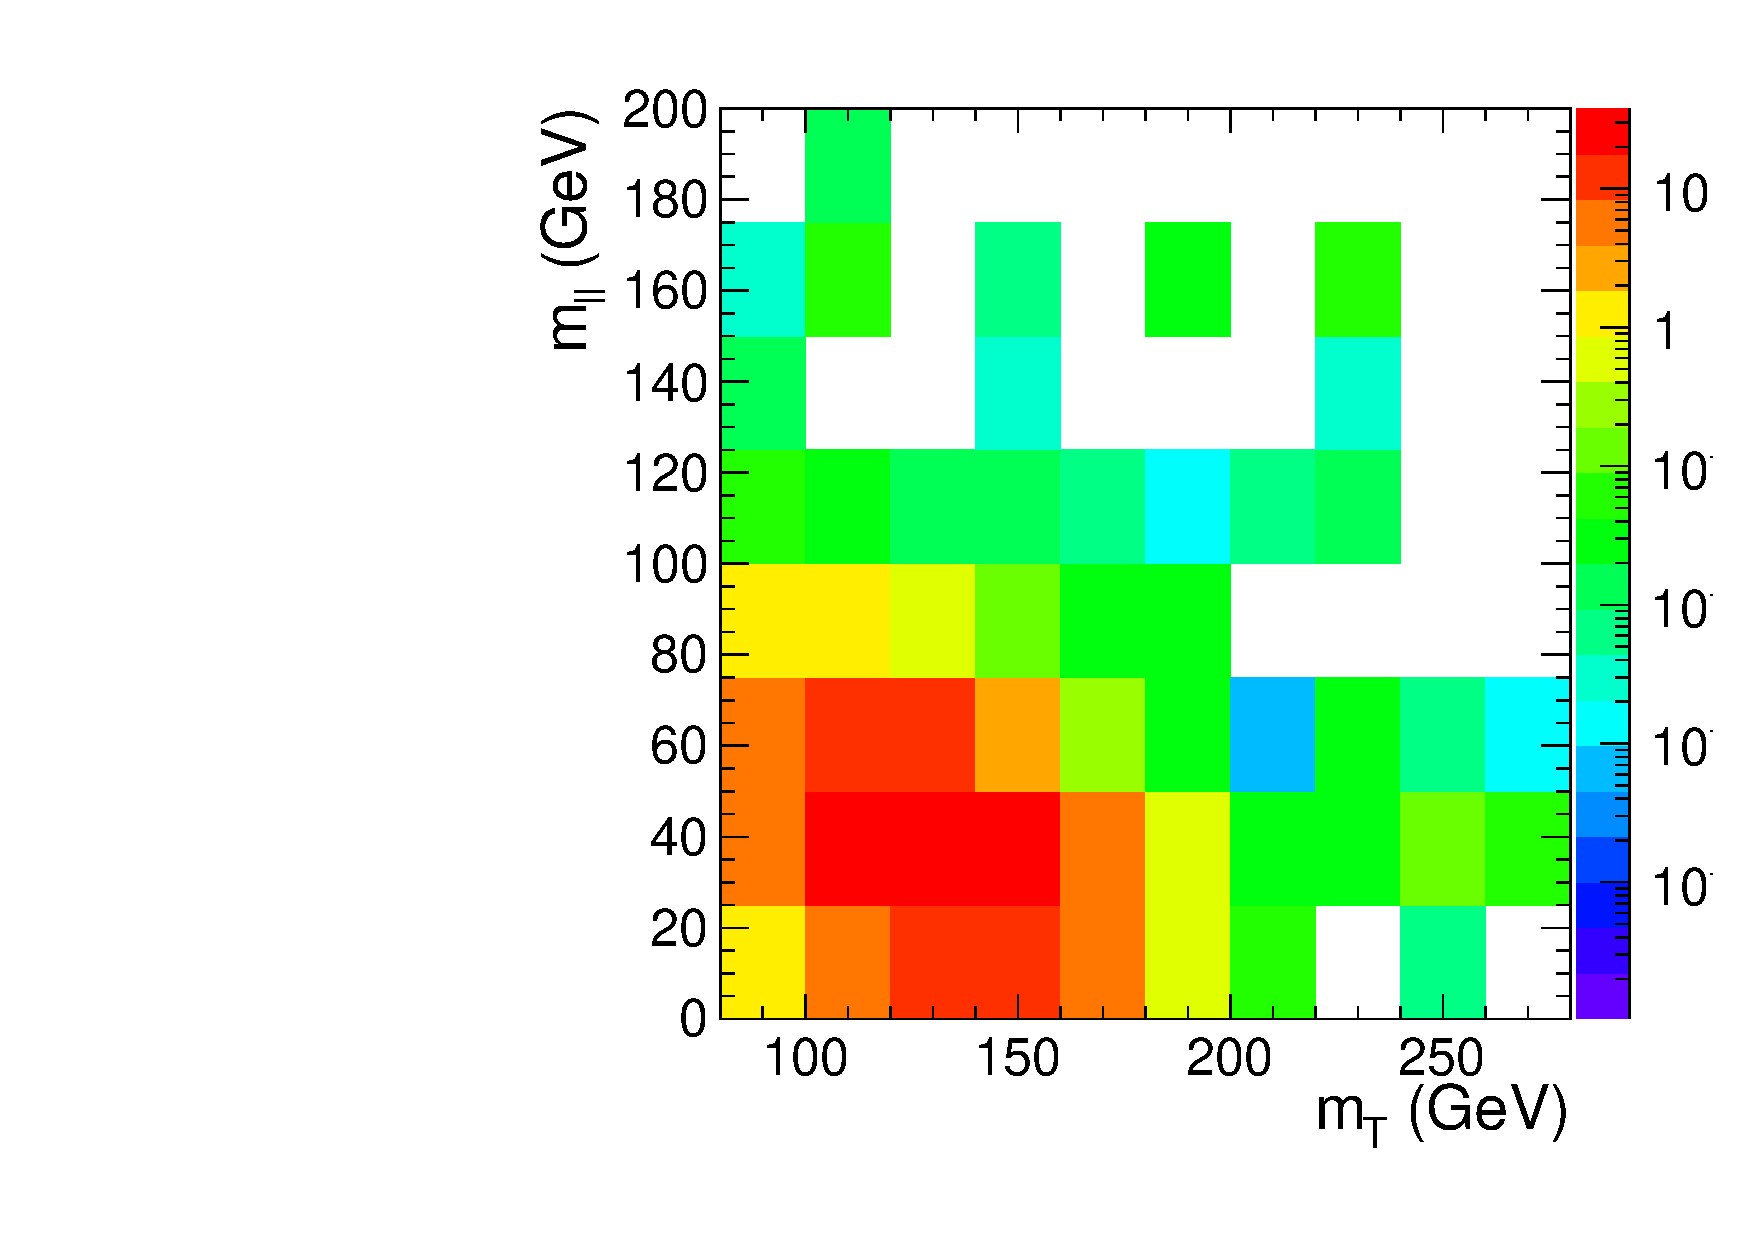
\includegraphics[width=.35\textwidth]{figures/templates/sig_2D_mH160_0j_of.pdf}
	}
	\subfigure[Signal statistical uncertainty]{
	\centering
	\label{subfig:template_signalerr_160}
		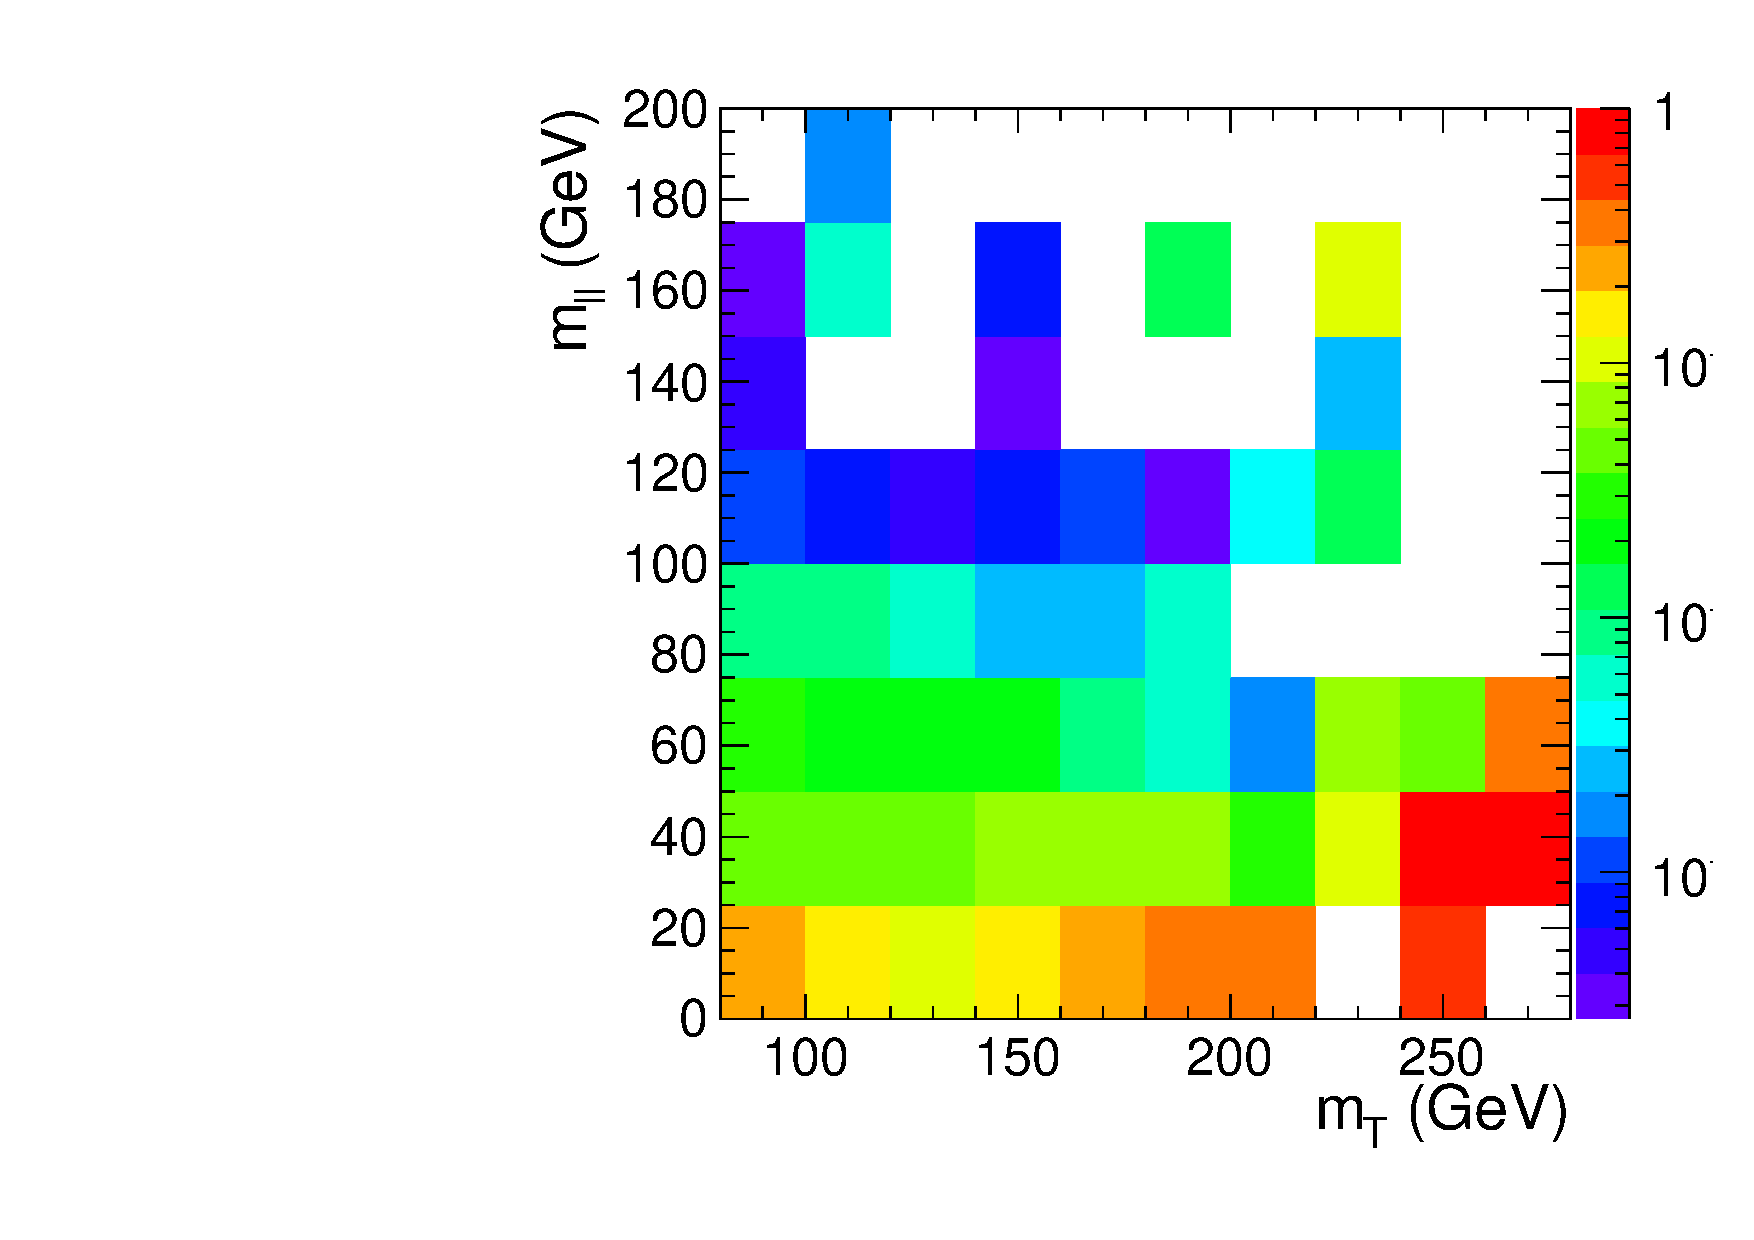
\includegraphics[width=.35\textwidth]{figures/templates/sigerr_2D_mH160_0j_of.pdf}
	}
	
	%
	\centering
	\subfigure[qqWW]{
	\centering
	\label{subfig:template_qqWW_160}
		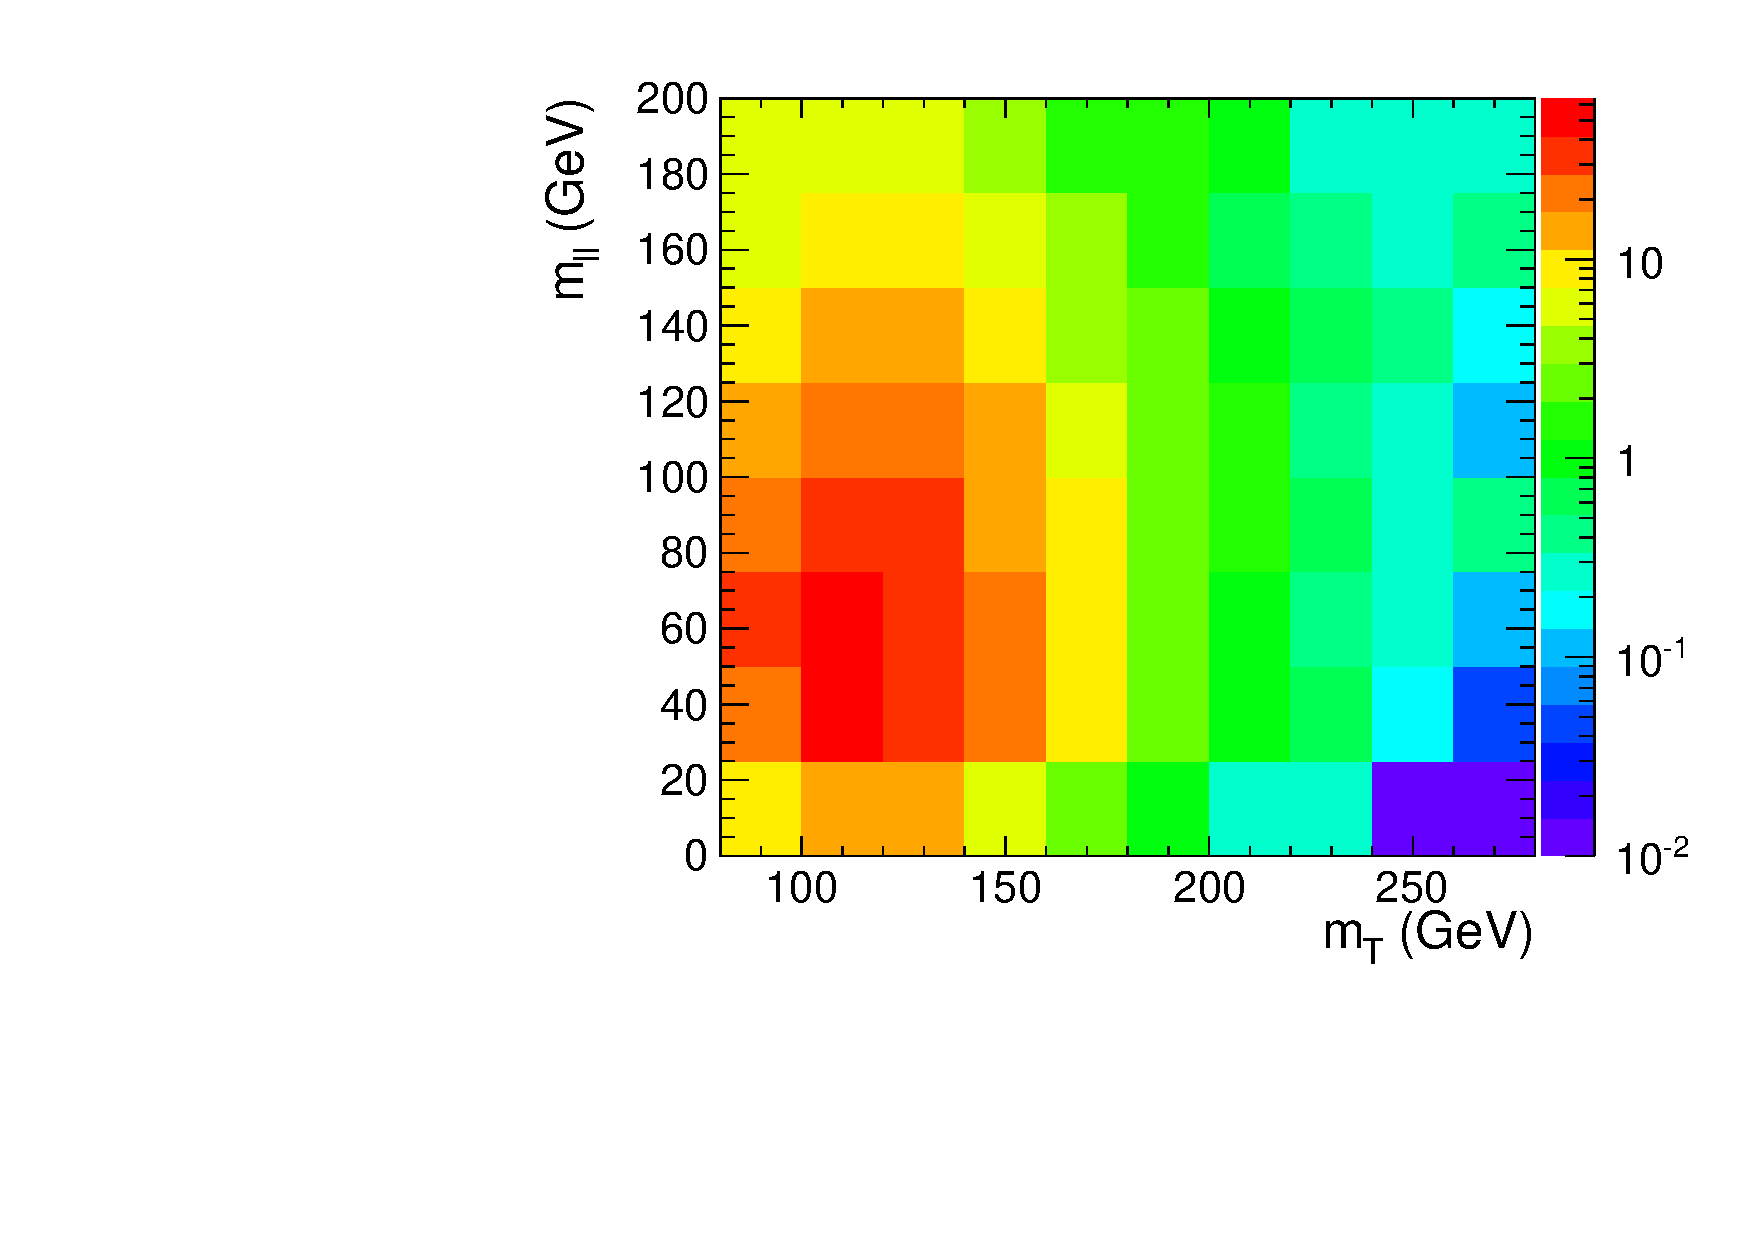
\includegraphics[width=.35\textwidth]{figures/templates/qqWW_2D_mH160_0j_of.pdf}
	}
	\subfigure[qqWW statistical uncertainty]{
	\centering
	\label{subfig:template_qqWWerr_160}
		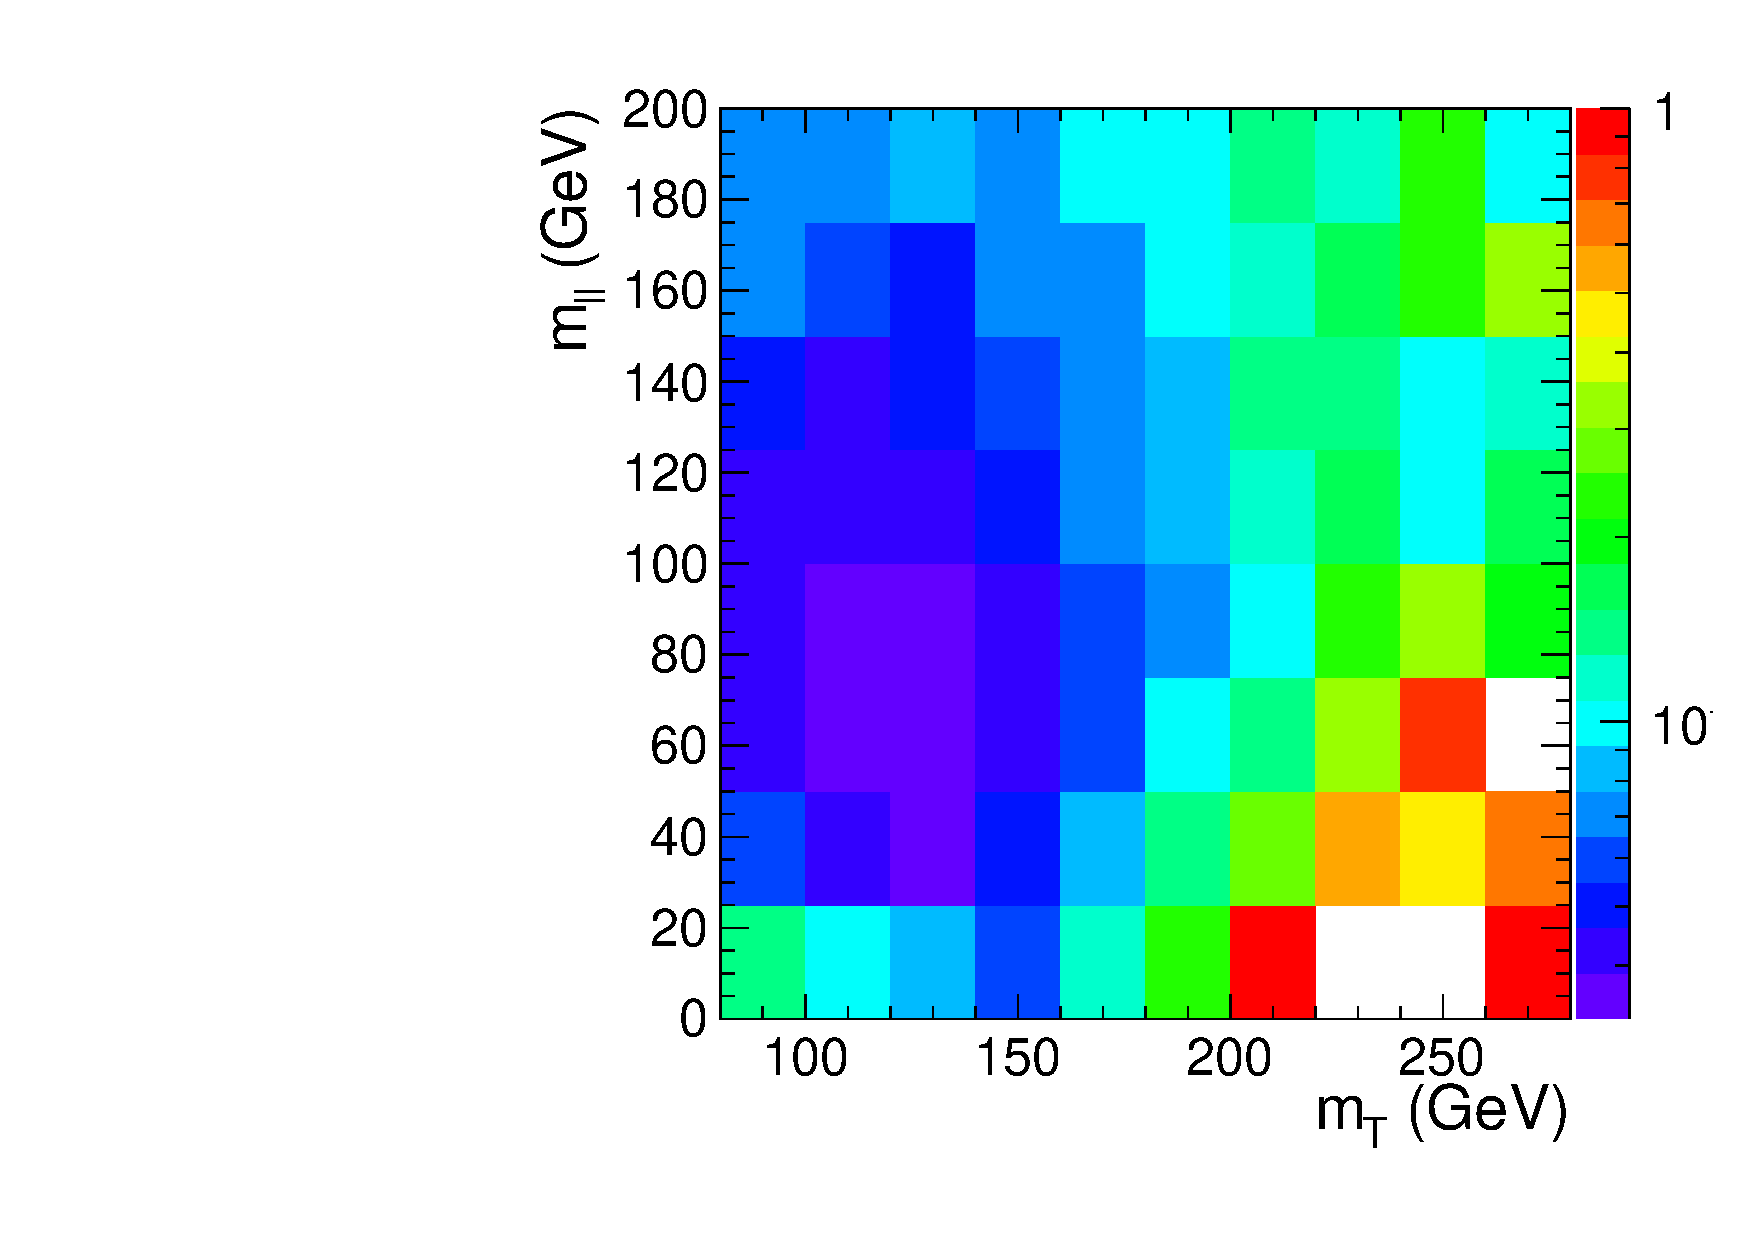
\includegraphics[width=.35\textwidth]{figures/templates/qqWWerr_2D_mH160_0j_of.pdf}
	}

	%
	\centering
	\subfigure[ggWW]{
	\centering
	\label{subfig:template_ggWW_160}
		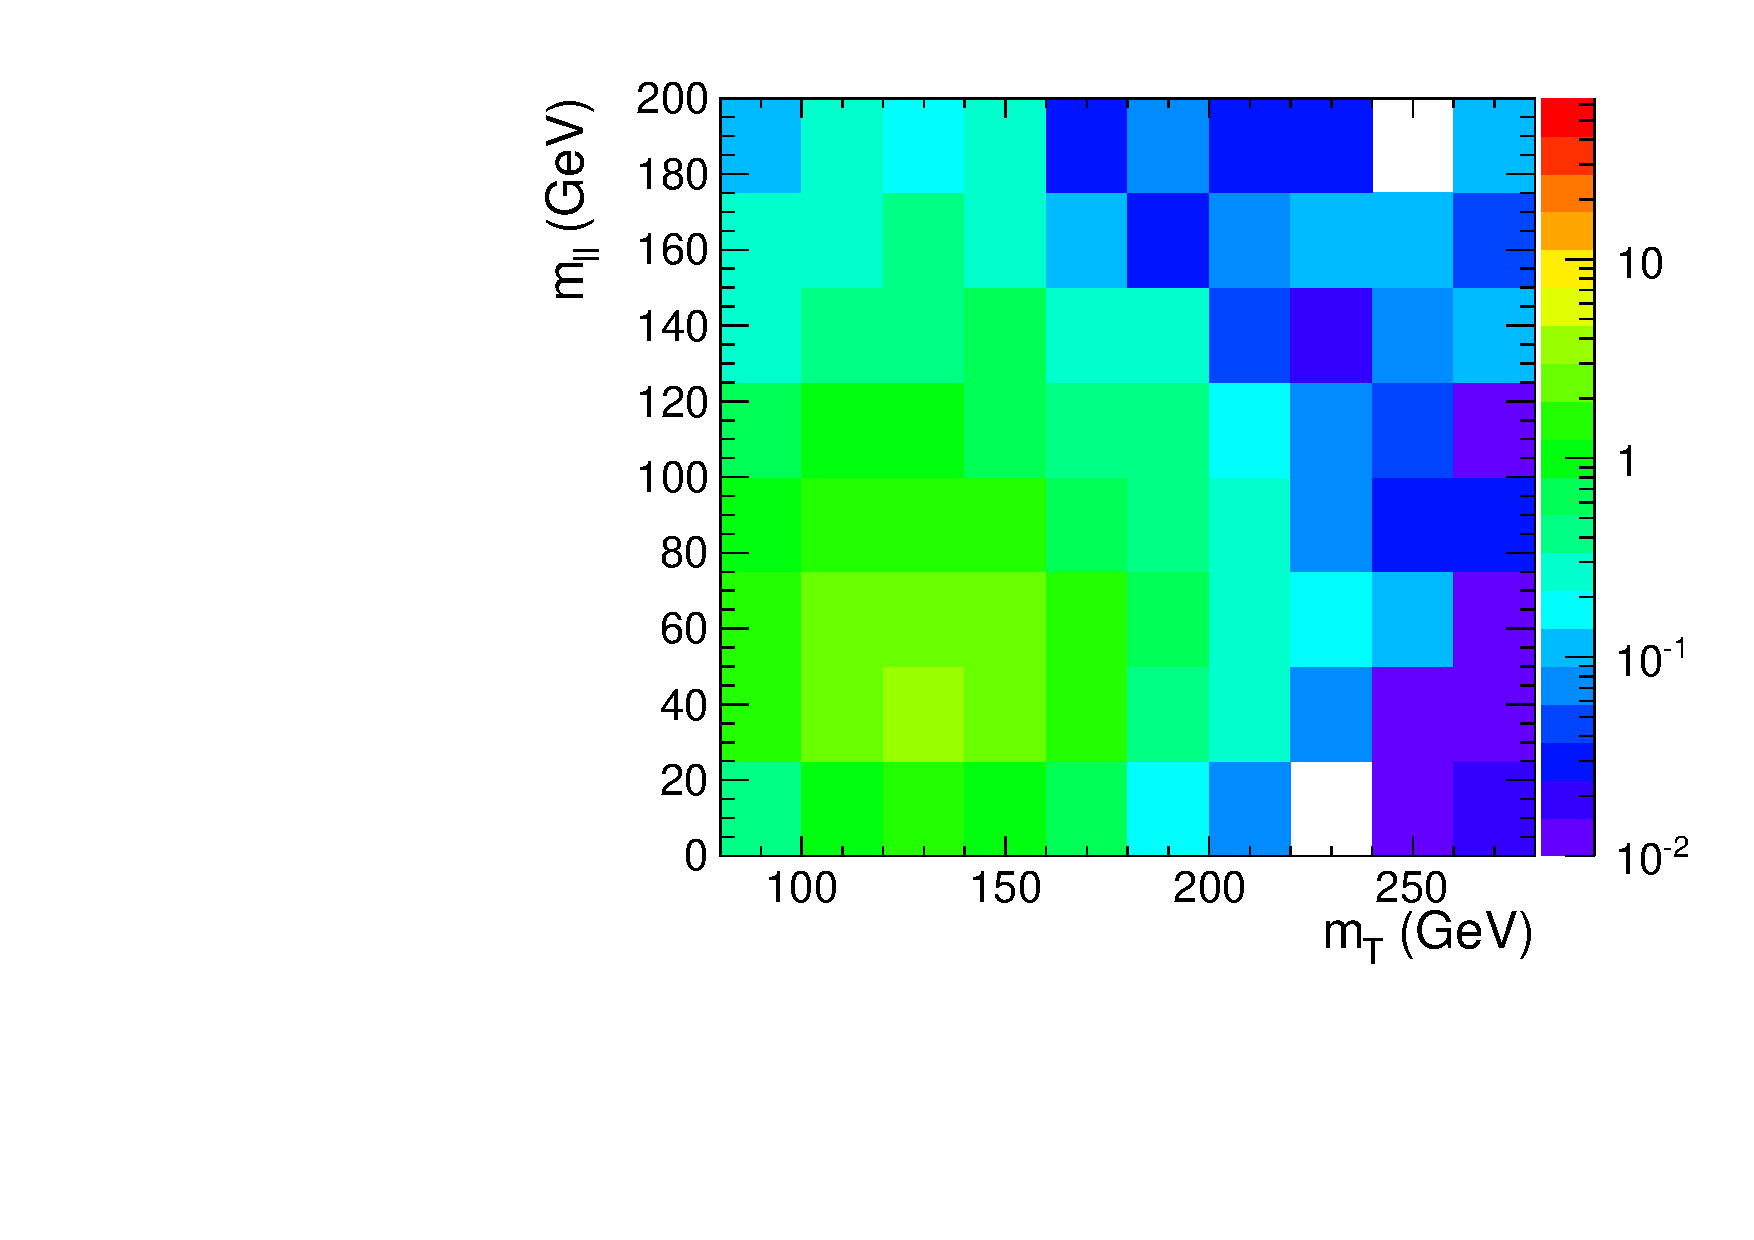
\includegraphics[width=.35\textwidth]{figures/templates/ggWW_2D_mH160_0j_of.pdf}
	}
	\subfigure[ggWW statistical uncertainty]{
	\centering
	\label{subfig:template_ggWWerr_160}
		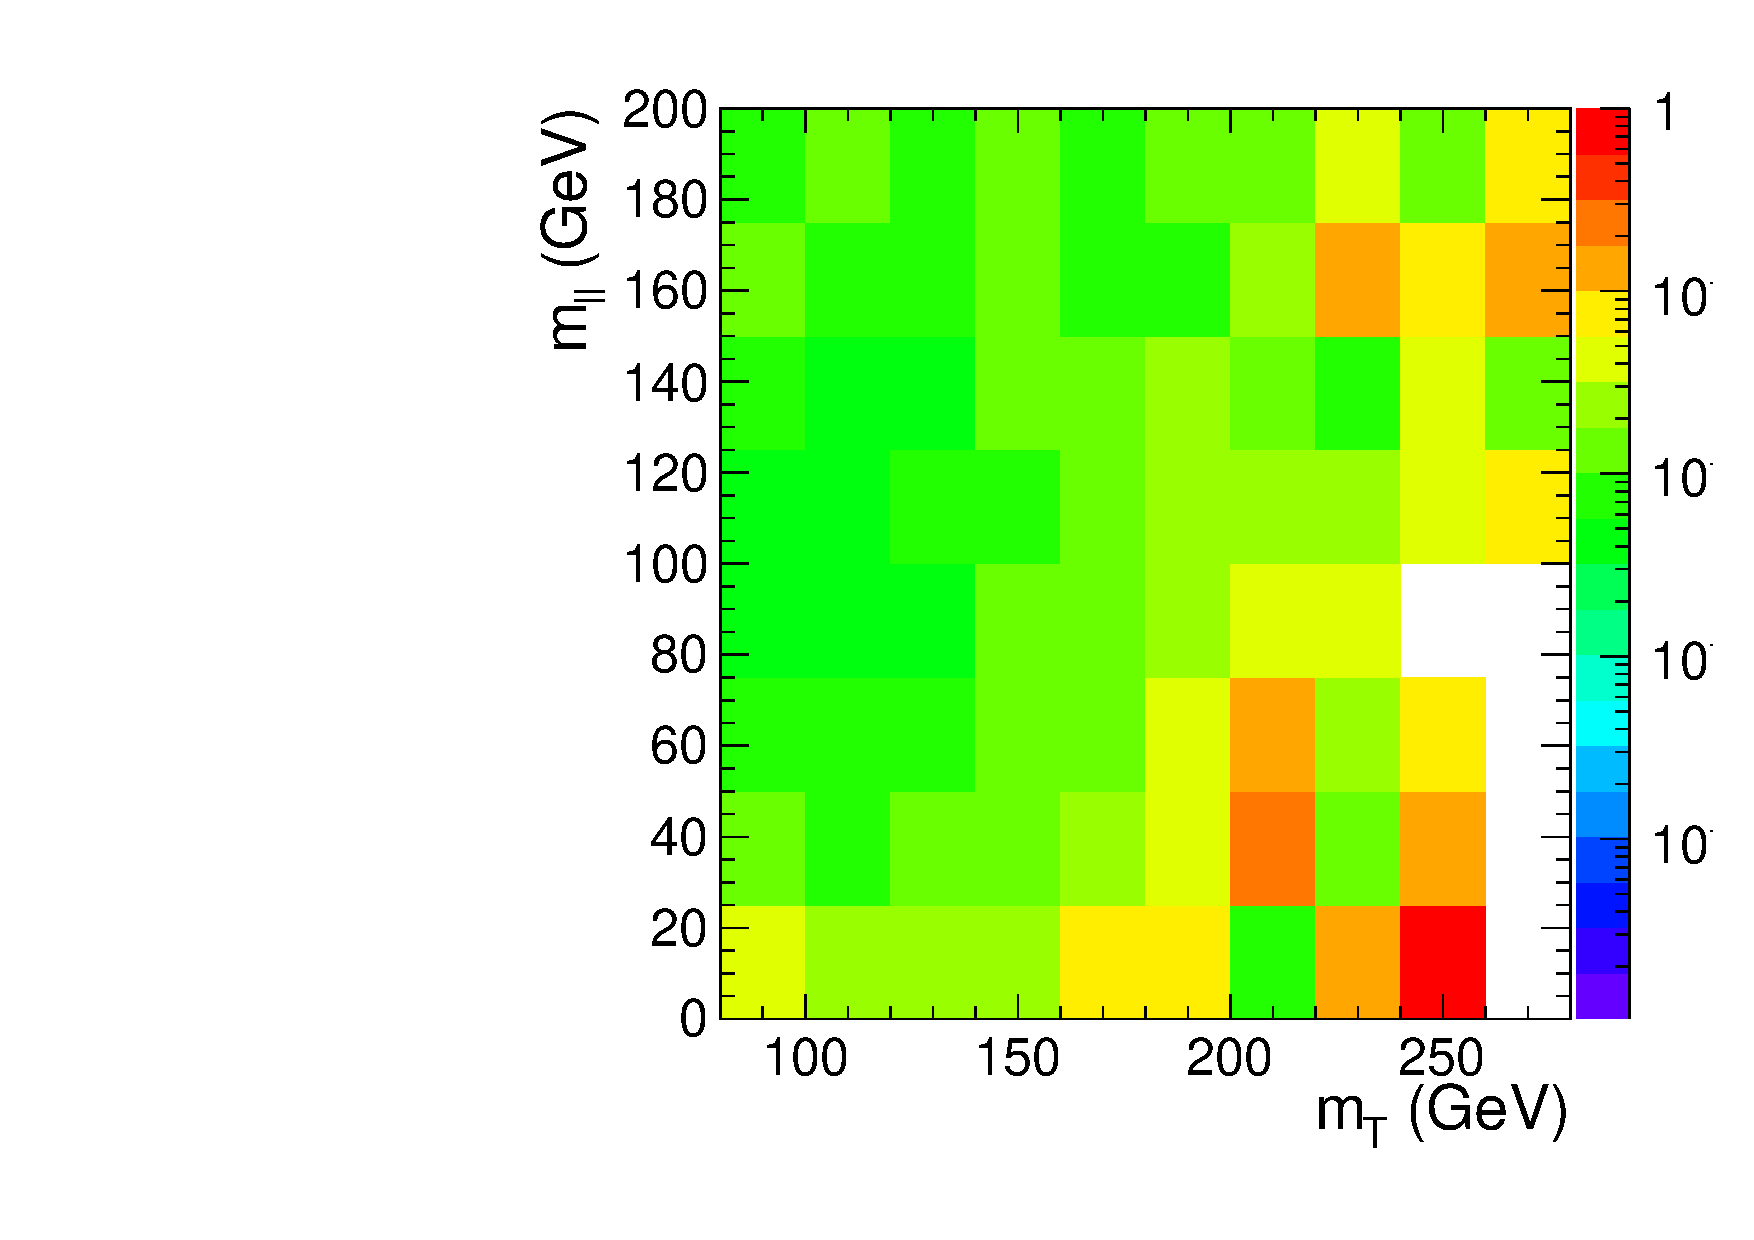
\includegraphics[width=.35\textwidth]{figures/templates/ggWWerr_2D_mH160_0j_of.pdf}
	}

	\caption{2D templates at \mHi = 160 \GeV} 
	\label{fig:templates_160_1}

\end{figure}

\begin{figure}[!hbtp]
	
	%
	\centering
	\subfigure[Wjets]{
	\centering
	\label{subfig:template_Wjets_160}
		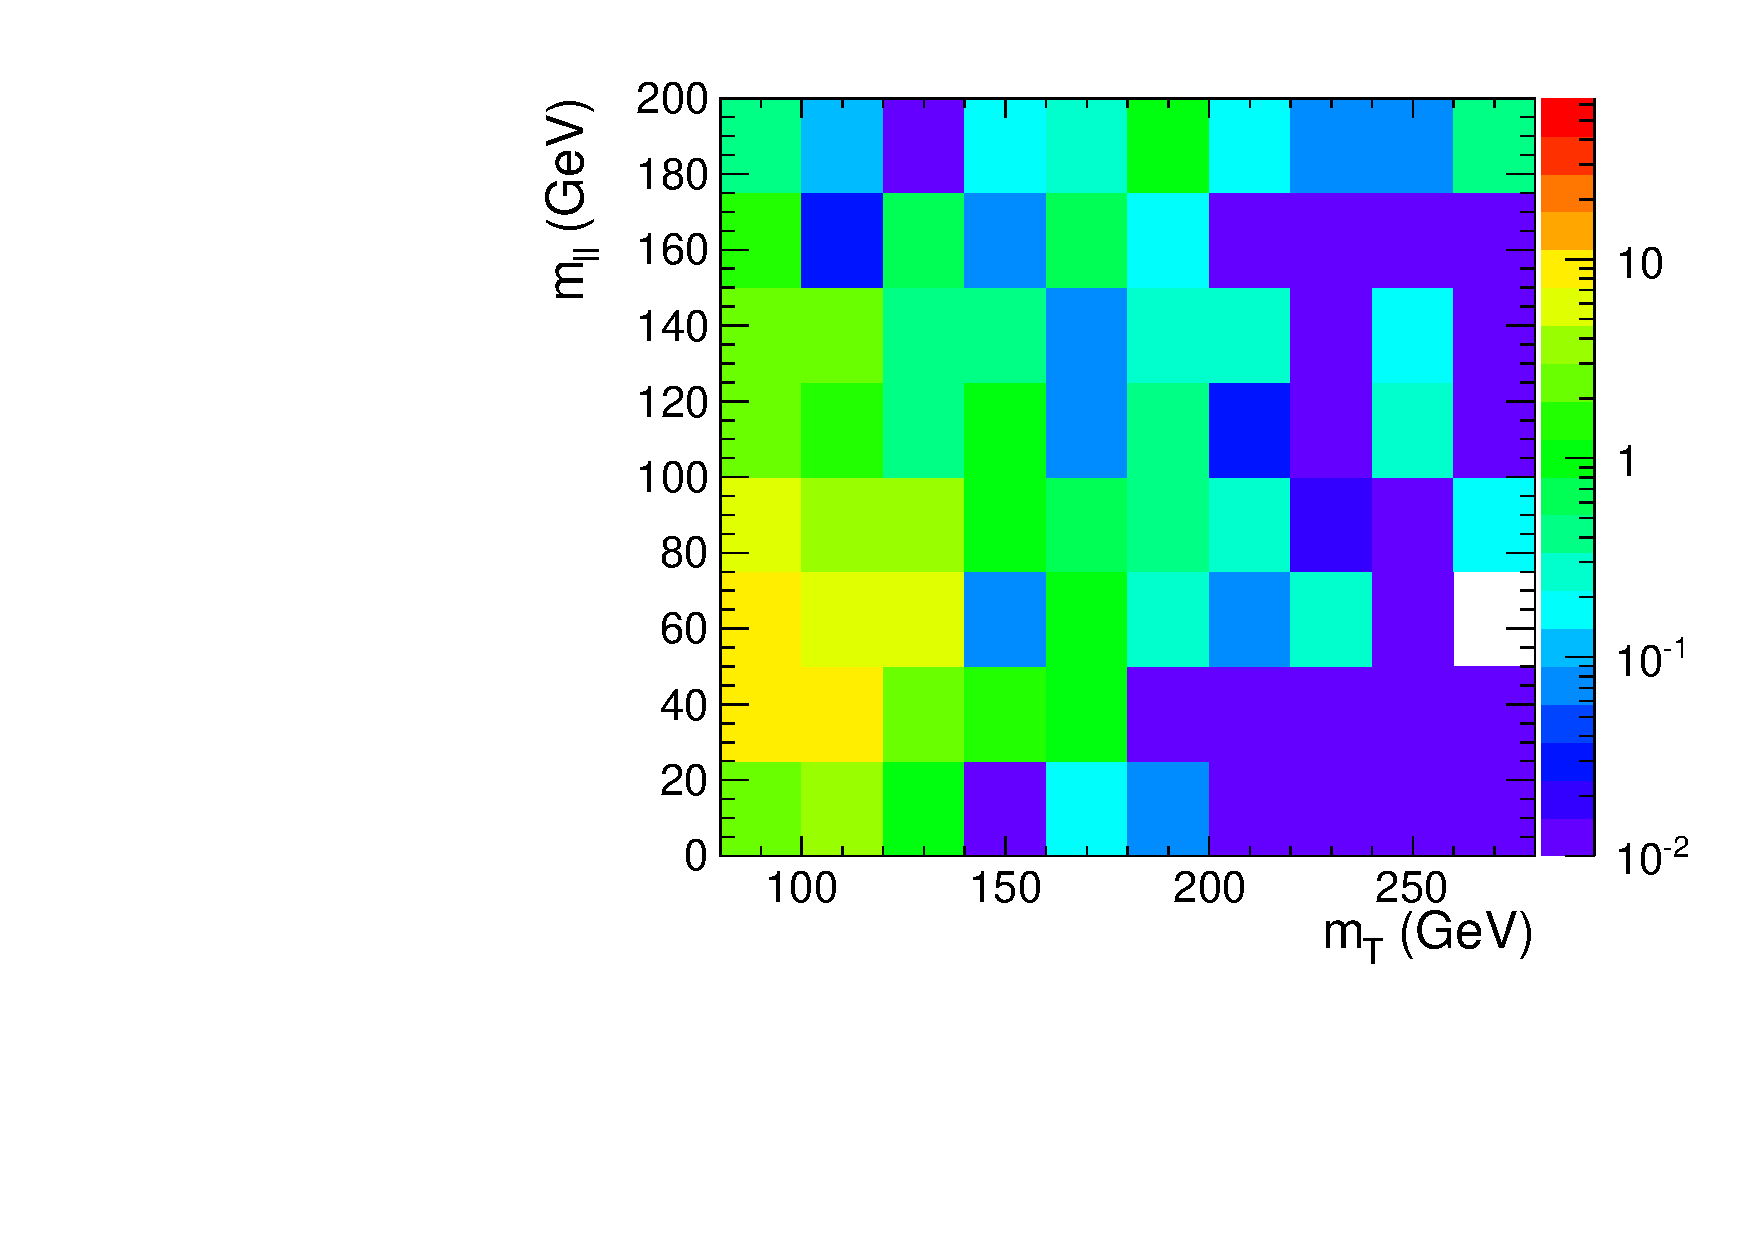
\includegraphics[width=.35\textwidth]{figures/templates/Wjets_2D_mH160_0j_of.pdf}
	}
	\subfigure[Wjets statistical uncertainty]{
	\centering
	\label{subfig:template_Wjetserr_160}
		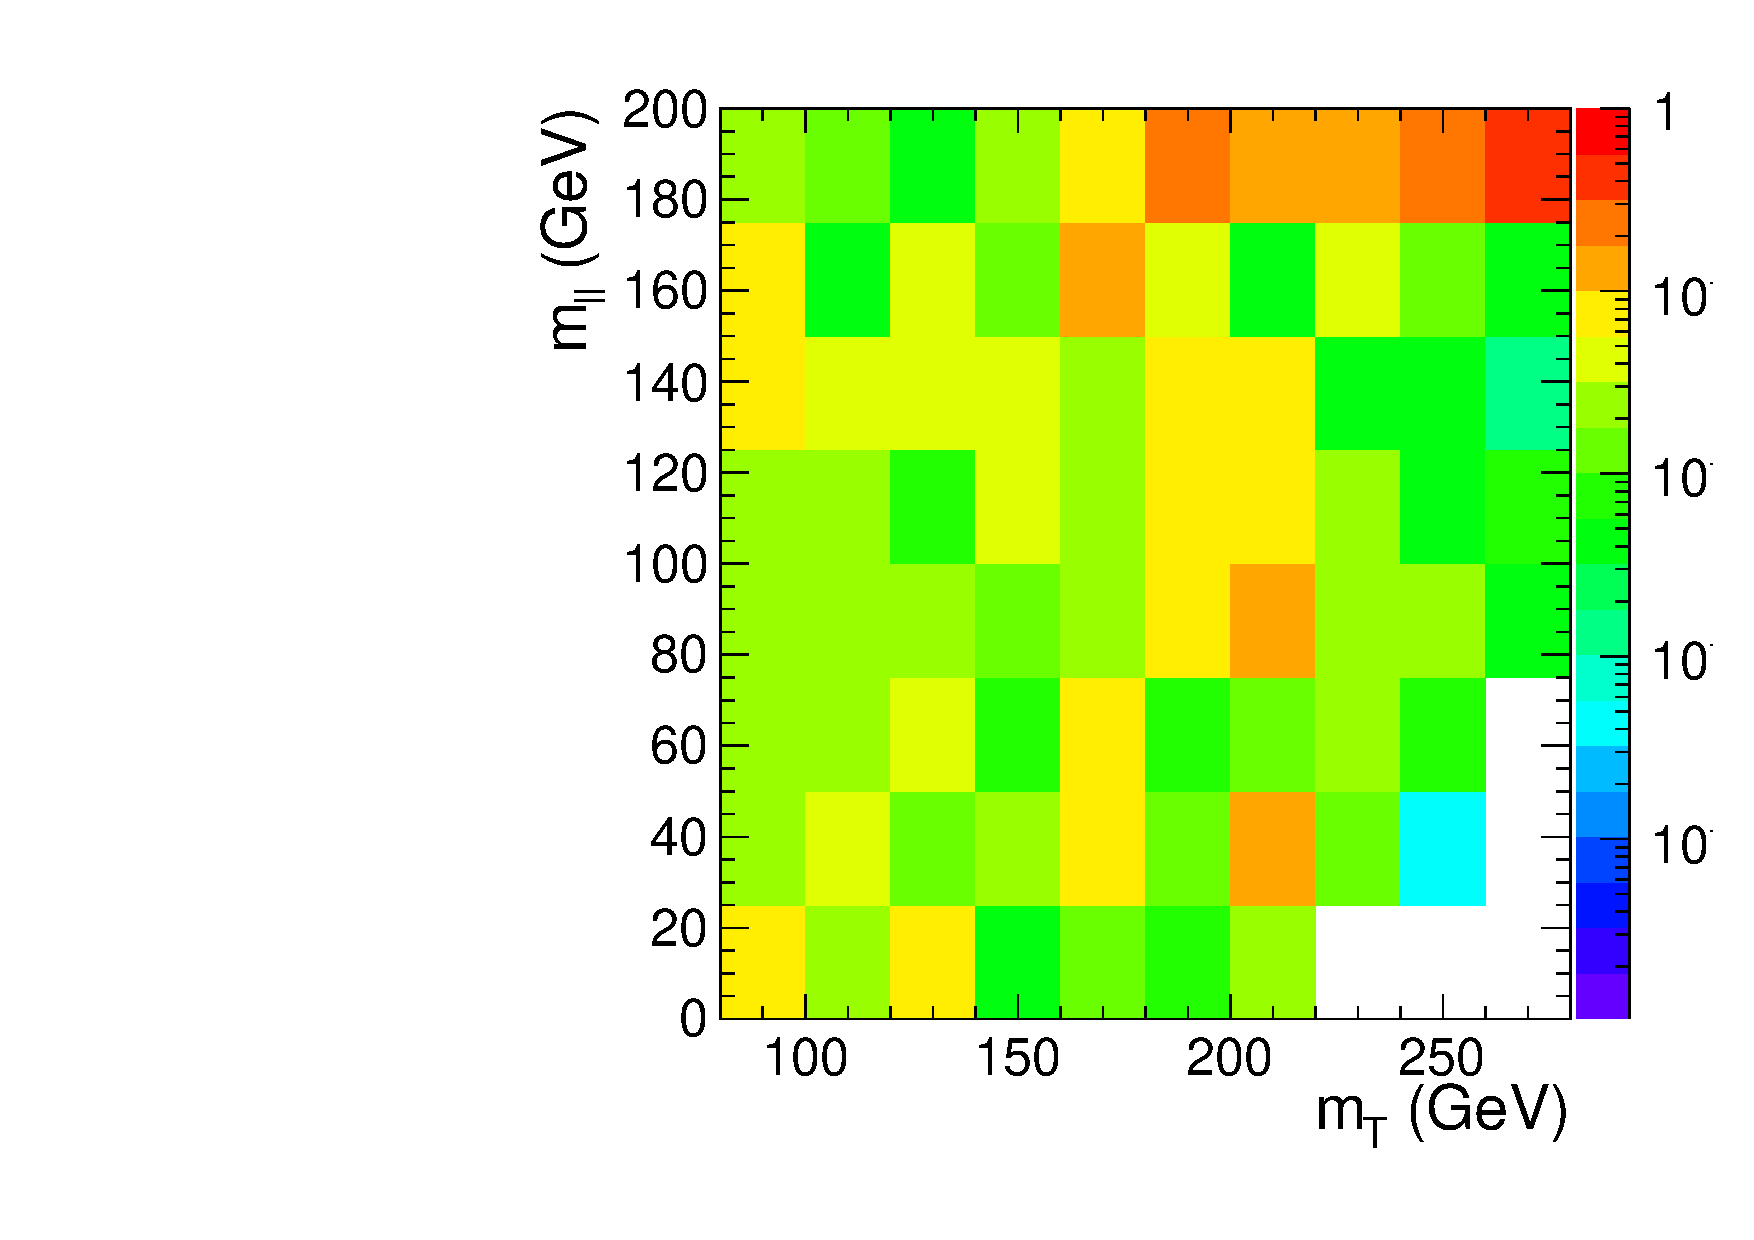
\includegraphics[width=.35\textwidth]{figures/templates/Wjetserr_2D_mH160_0j_of.pdf}
	}
	
	%
	\centering
	\subfigure[Top]{
	\centering
	\label{subfig:template_Top_160}
		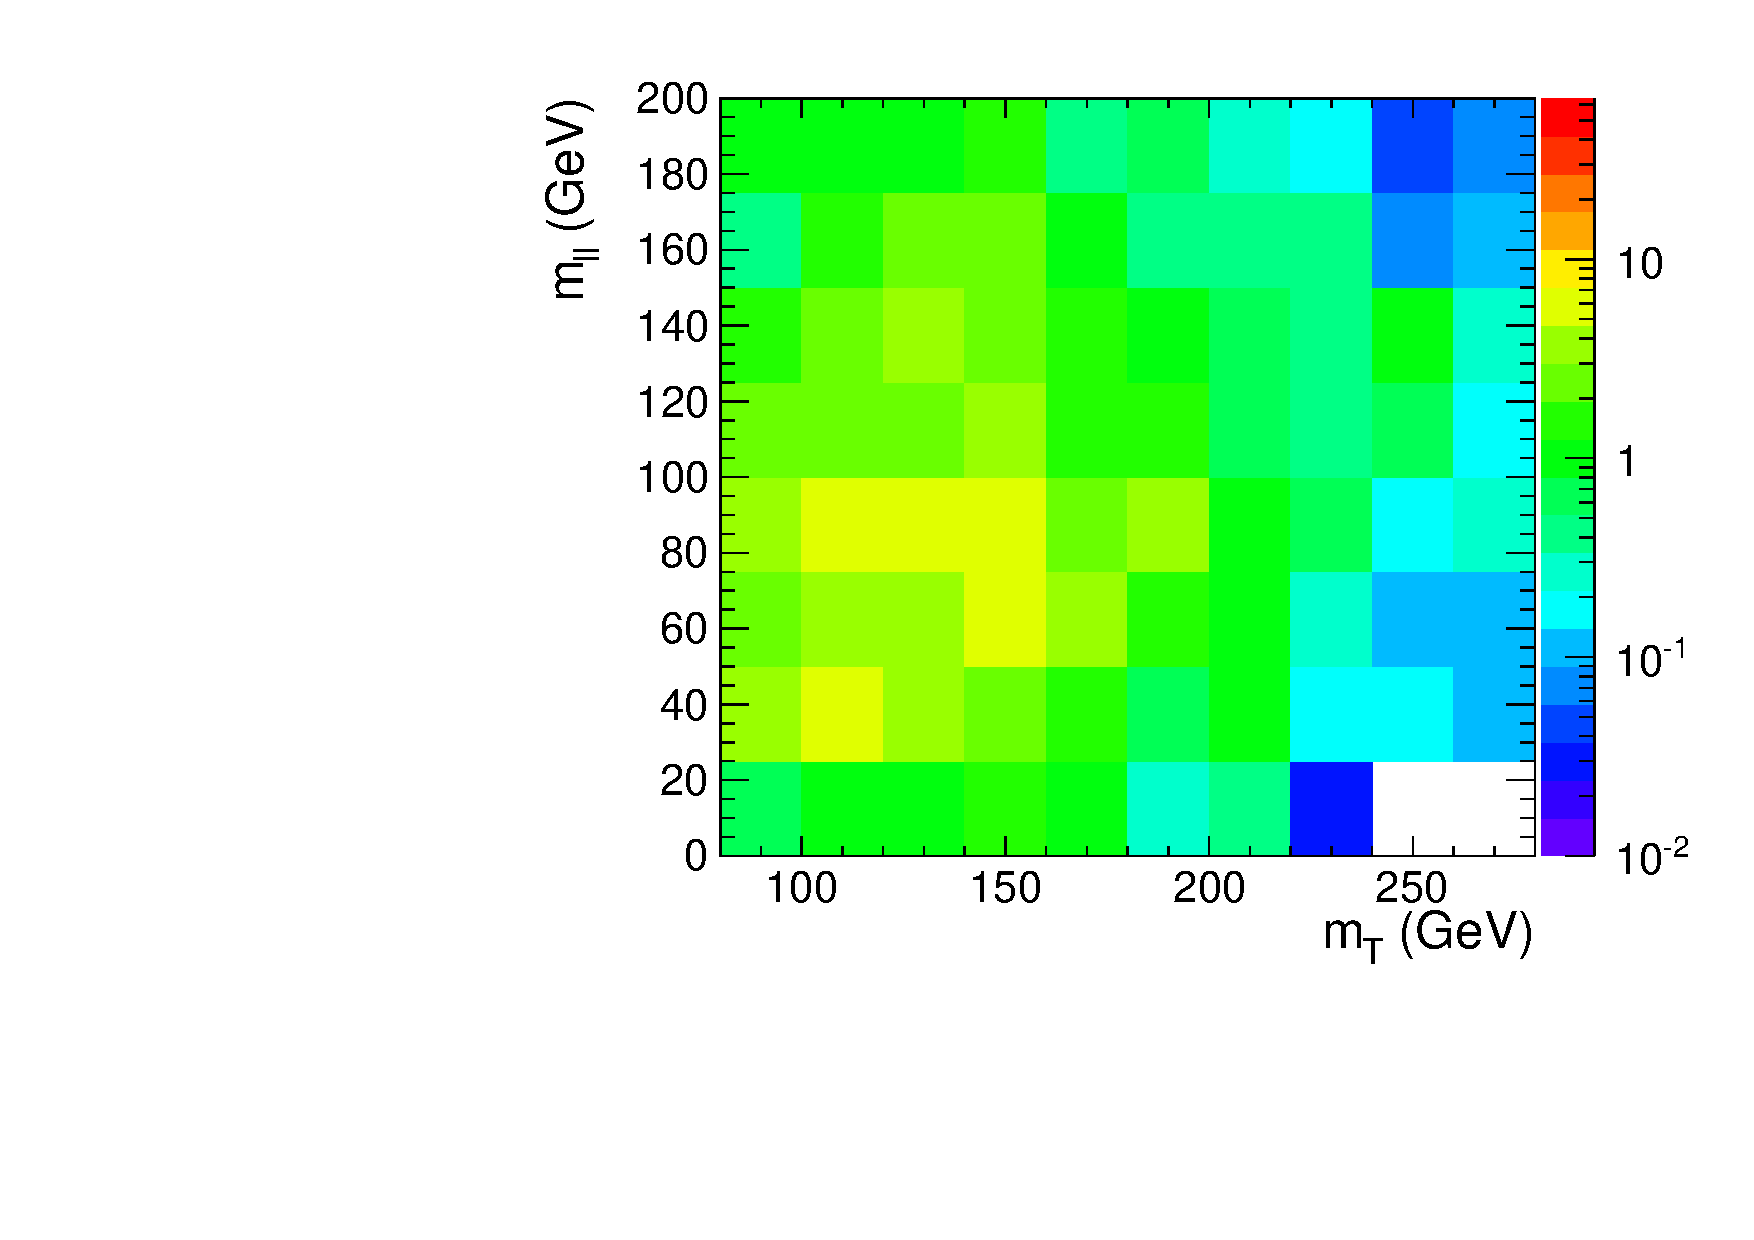
\includegraphics[width=.35\textwidth]{figures/templates/Top_2D_mH160_0j_of.pdf}
	}
	\subfigure[Top statistical uncertainty]{
	\centering
	\label{subfig:template_Toperr_160}
		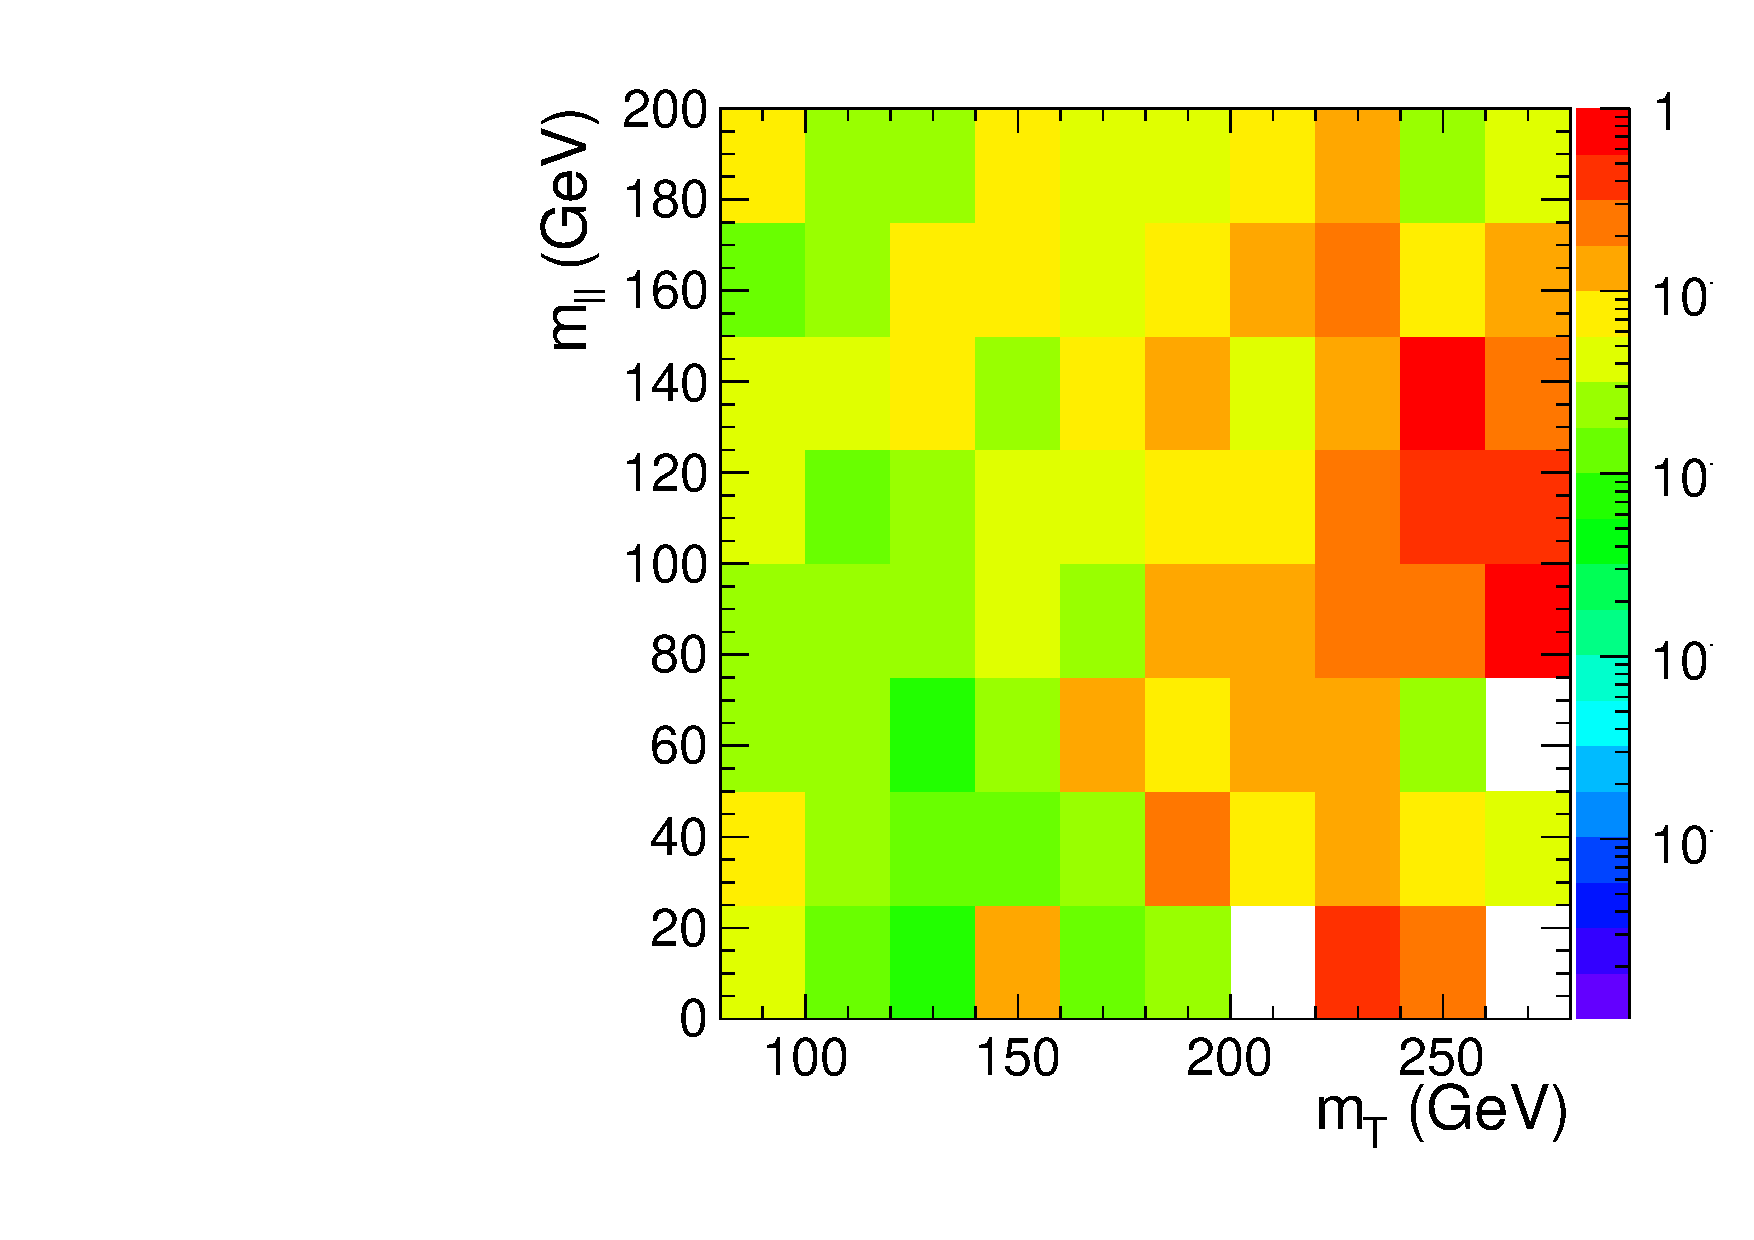
\includegraphics[width=.35\textwidth]{figures/templates/Toperr_2D_mH160_0j_of.pdf}
	}

	%
	\centering
	\subfigure[VV]{
	\centering
	\label{subfig:template_VV_160}
		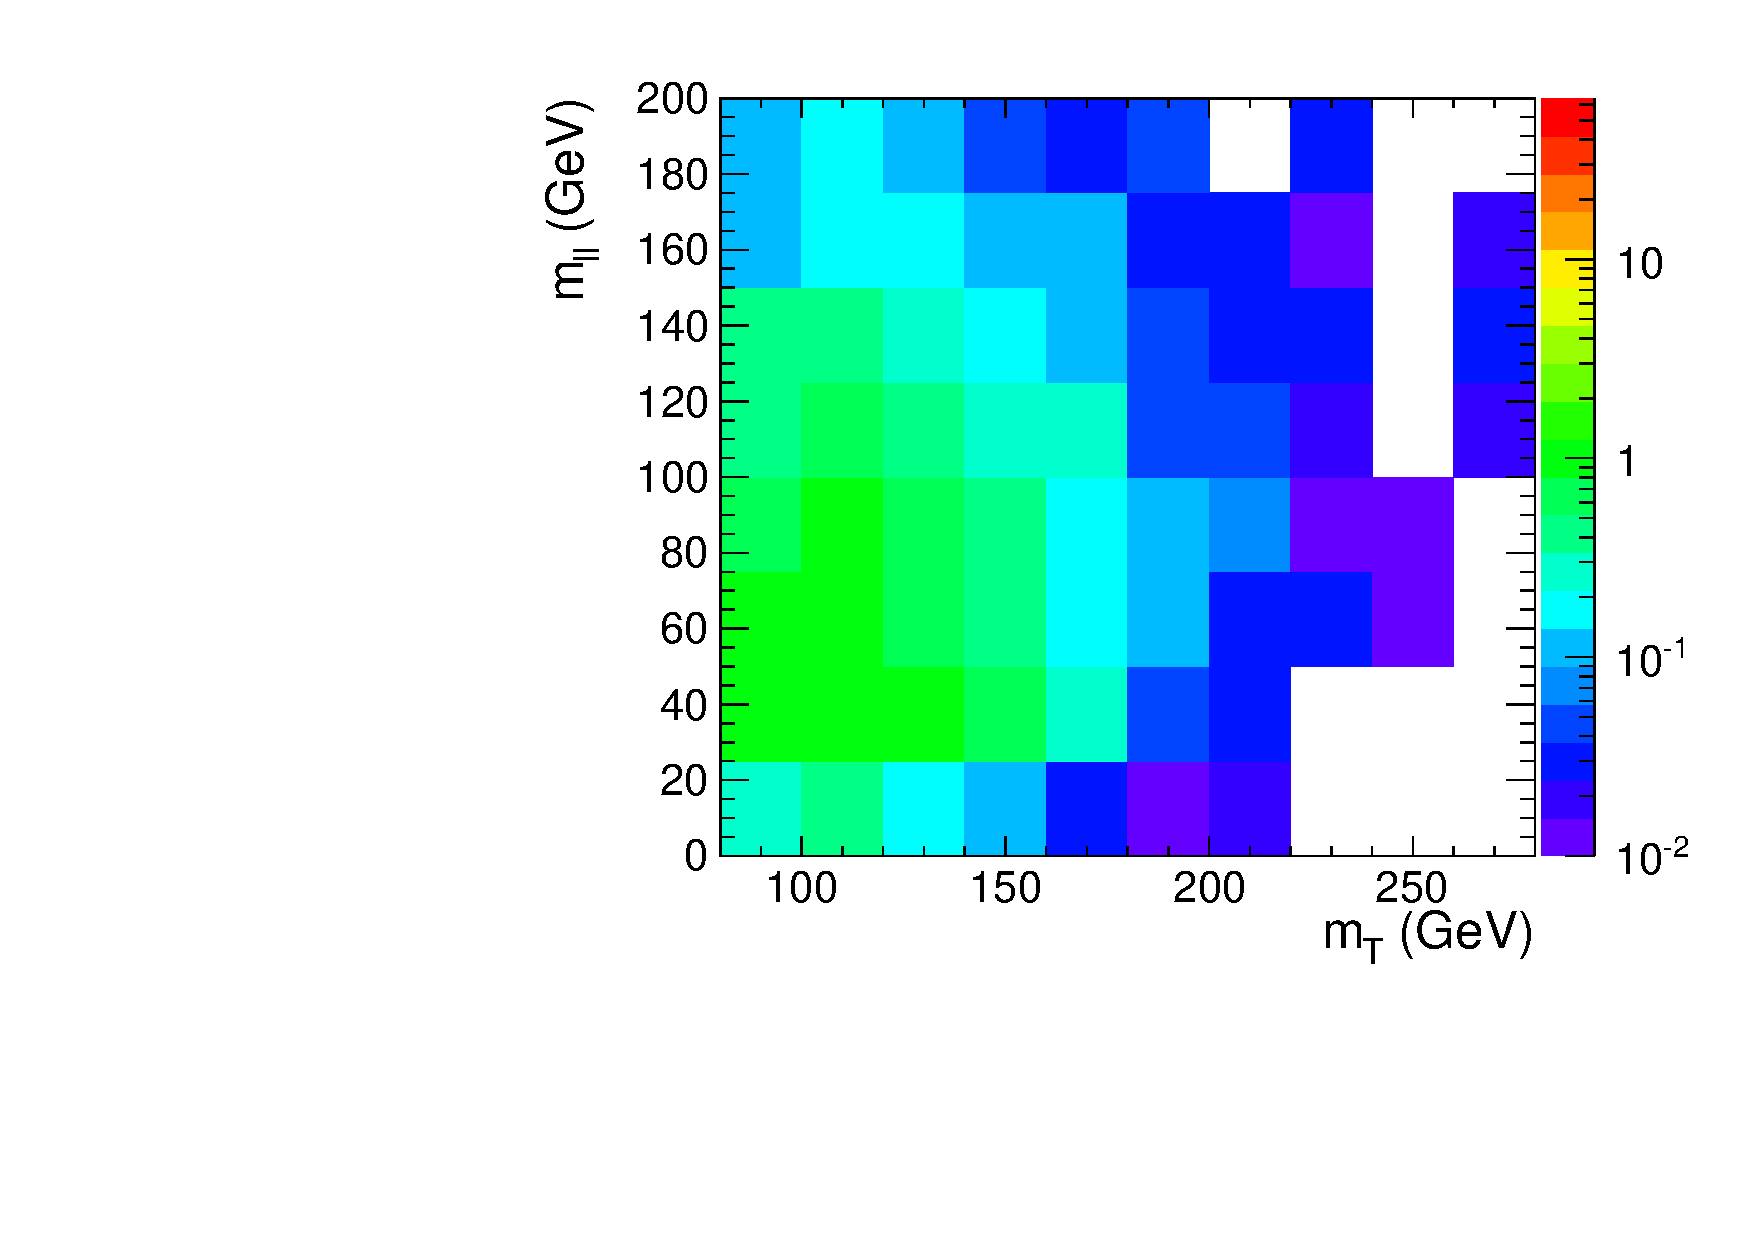
\includegraphics[width=.35\textwidth]{figures/templates/VV_2D_mH160_0j_of.pdf}
	}
	\subfigure[VV statistical uncertainty]{
	\centering
	\label{subfig:template_VVerr_160}
		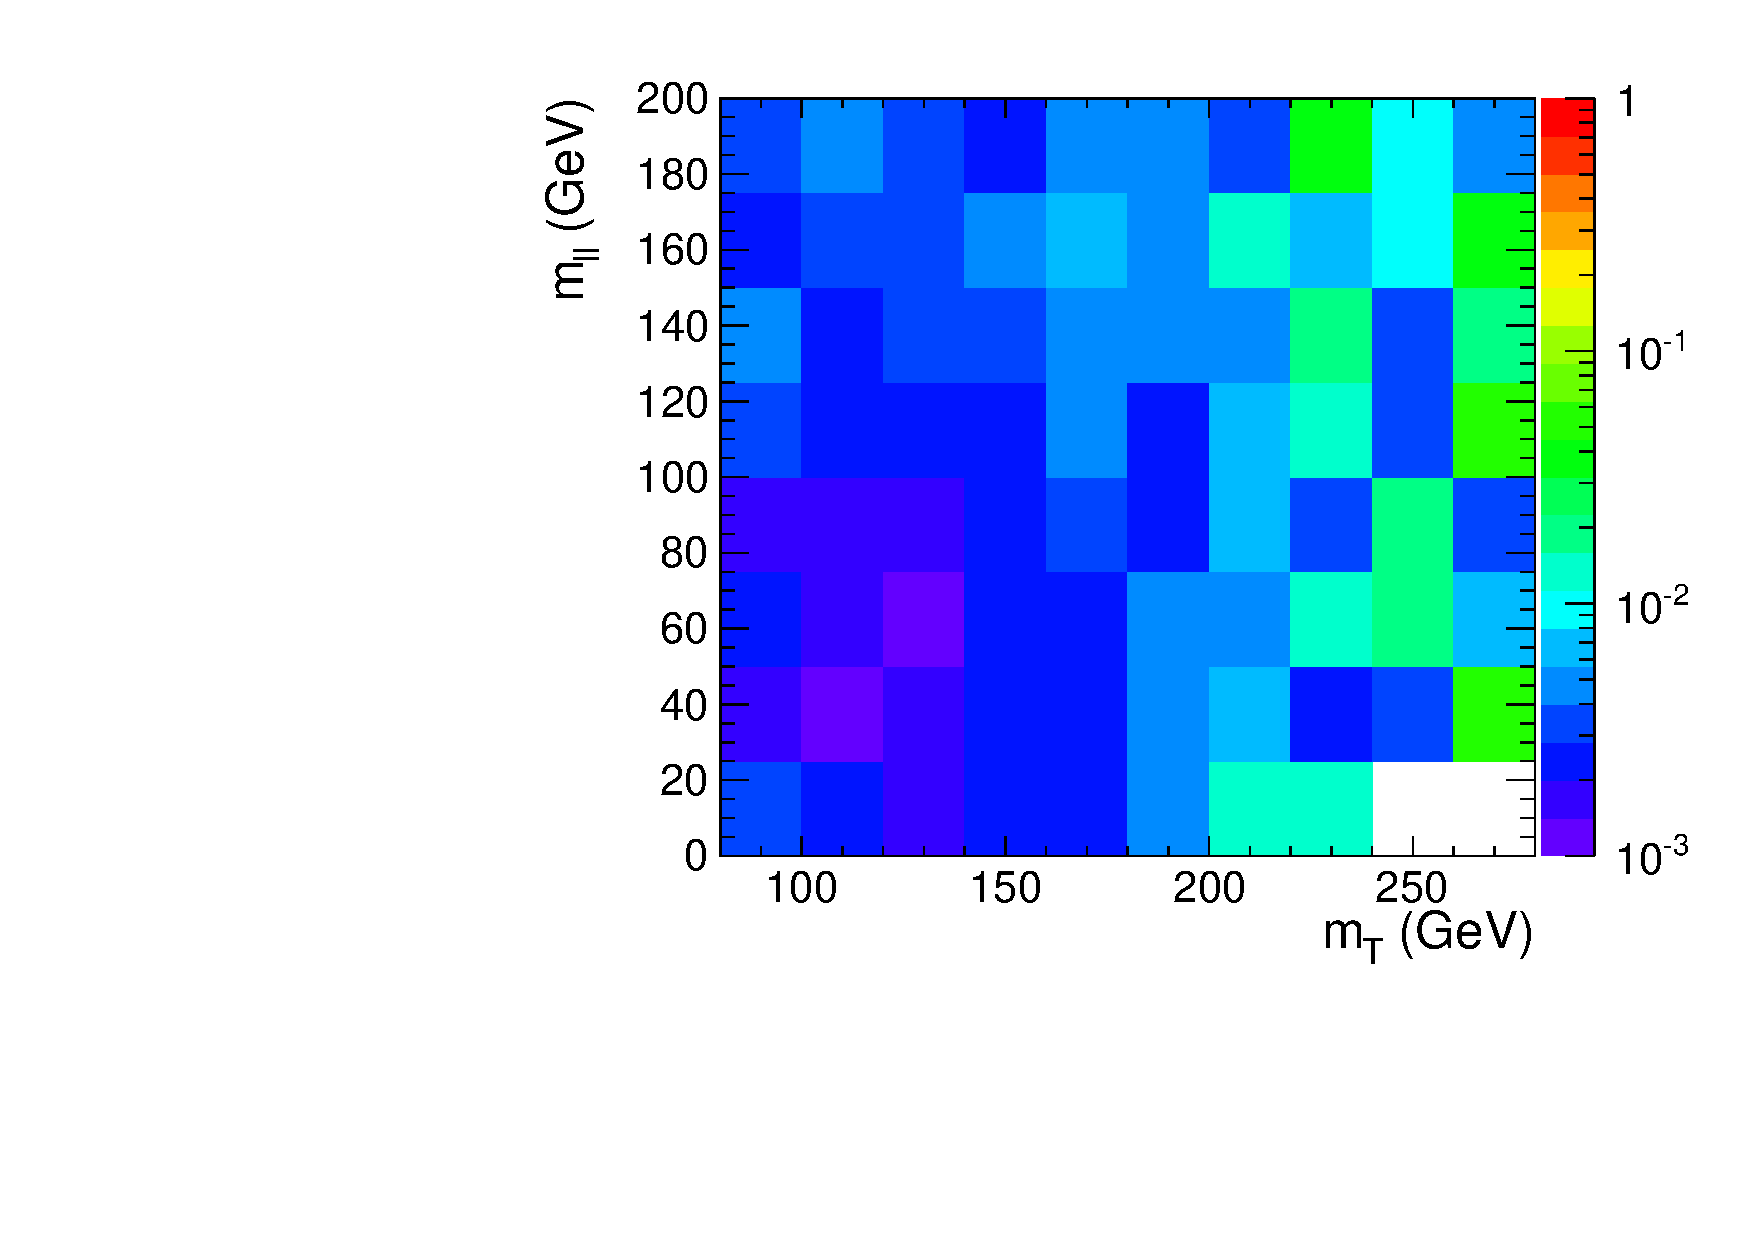
\includegraphics[width=.35\textwidth]{figures/templates/VVerr_2D_mH160_0j_of.pdf}
	}

	\caption{2D templates at \mHi = 160 \GeV} 
	\label{fig:templates_160_2}

\end{figure}

\begin{figure}[!hbtp]
	
	%
	\centering
	\subfigure[Zjets]{
	\centering
	\label{subfig:template_Zjets_160}
		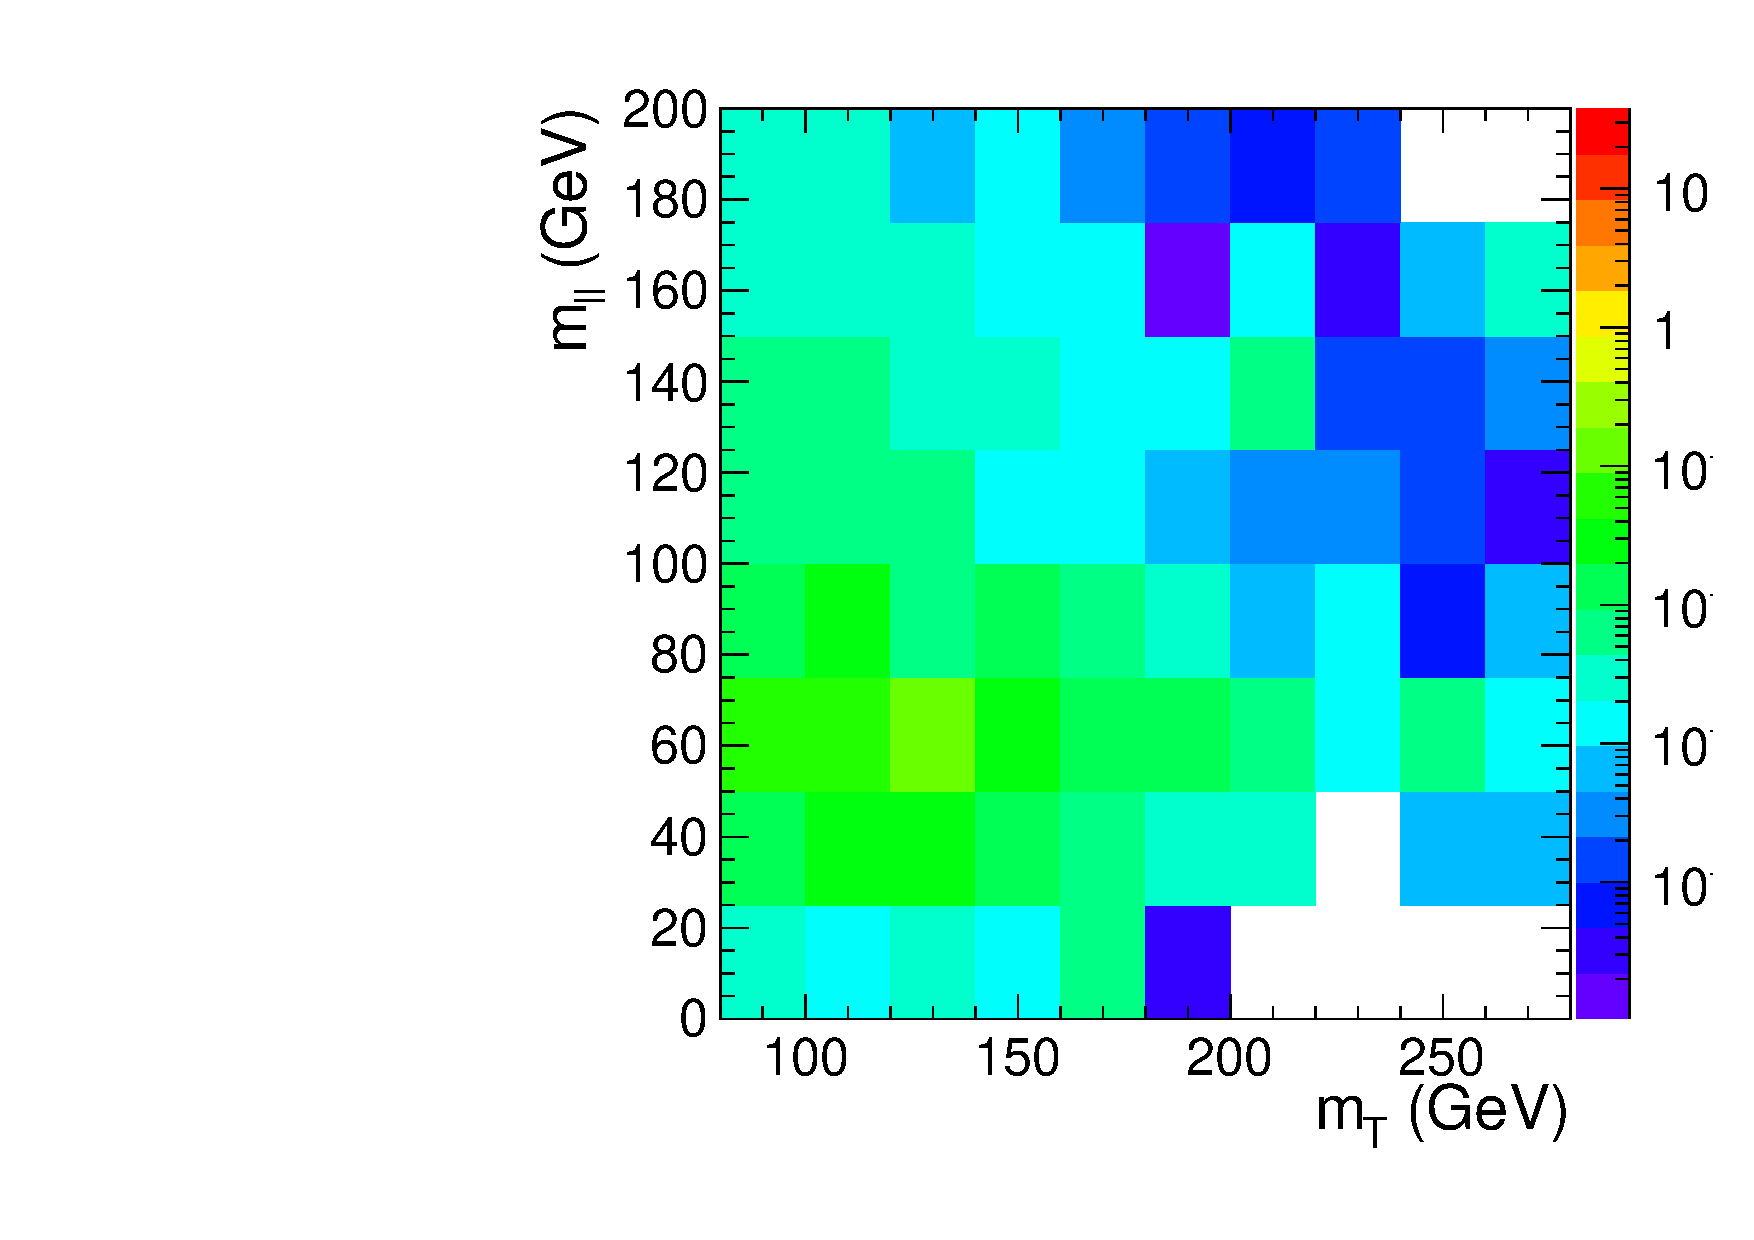
\includegraphics[width=.35\textwidth]{figures/templates/Zjets_2D_mH160_0j_of.pdf}
	}
	\subfigure[Zjets statistical uncertainty]{
	\centering
	\label{subfig:template_Zjetserr_160}
		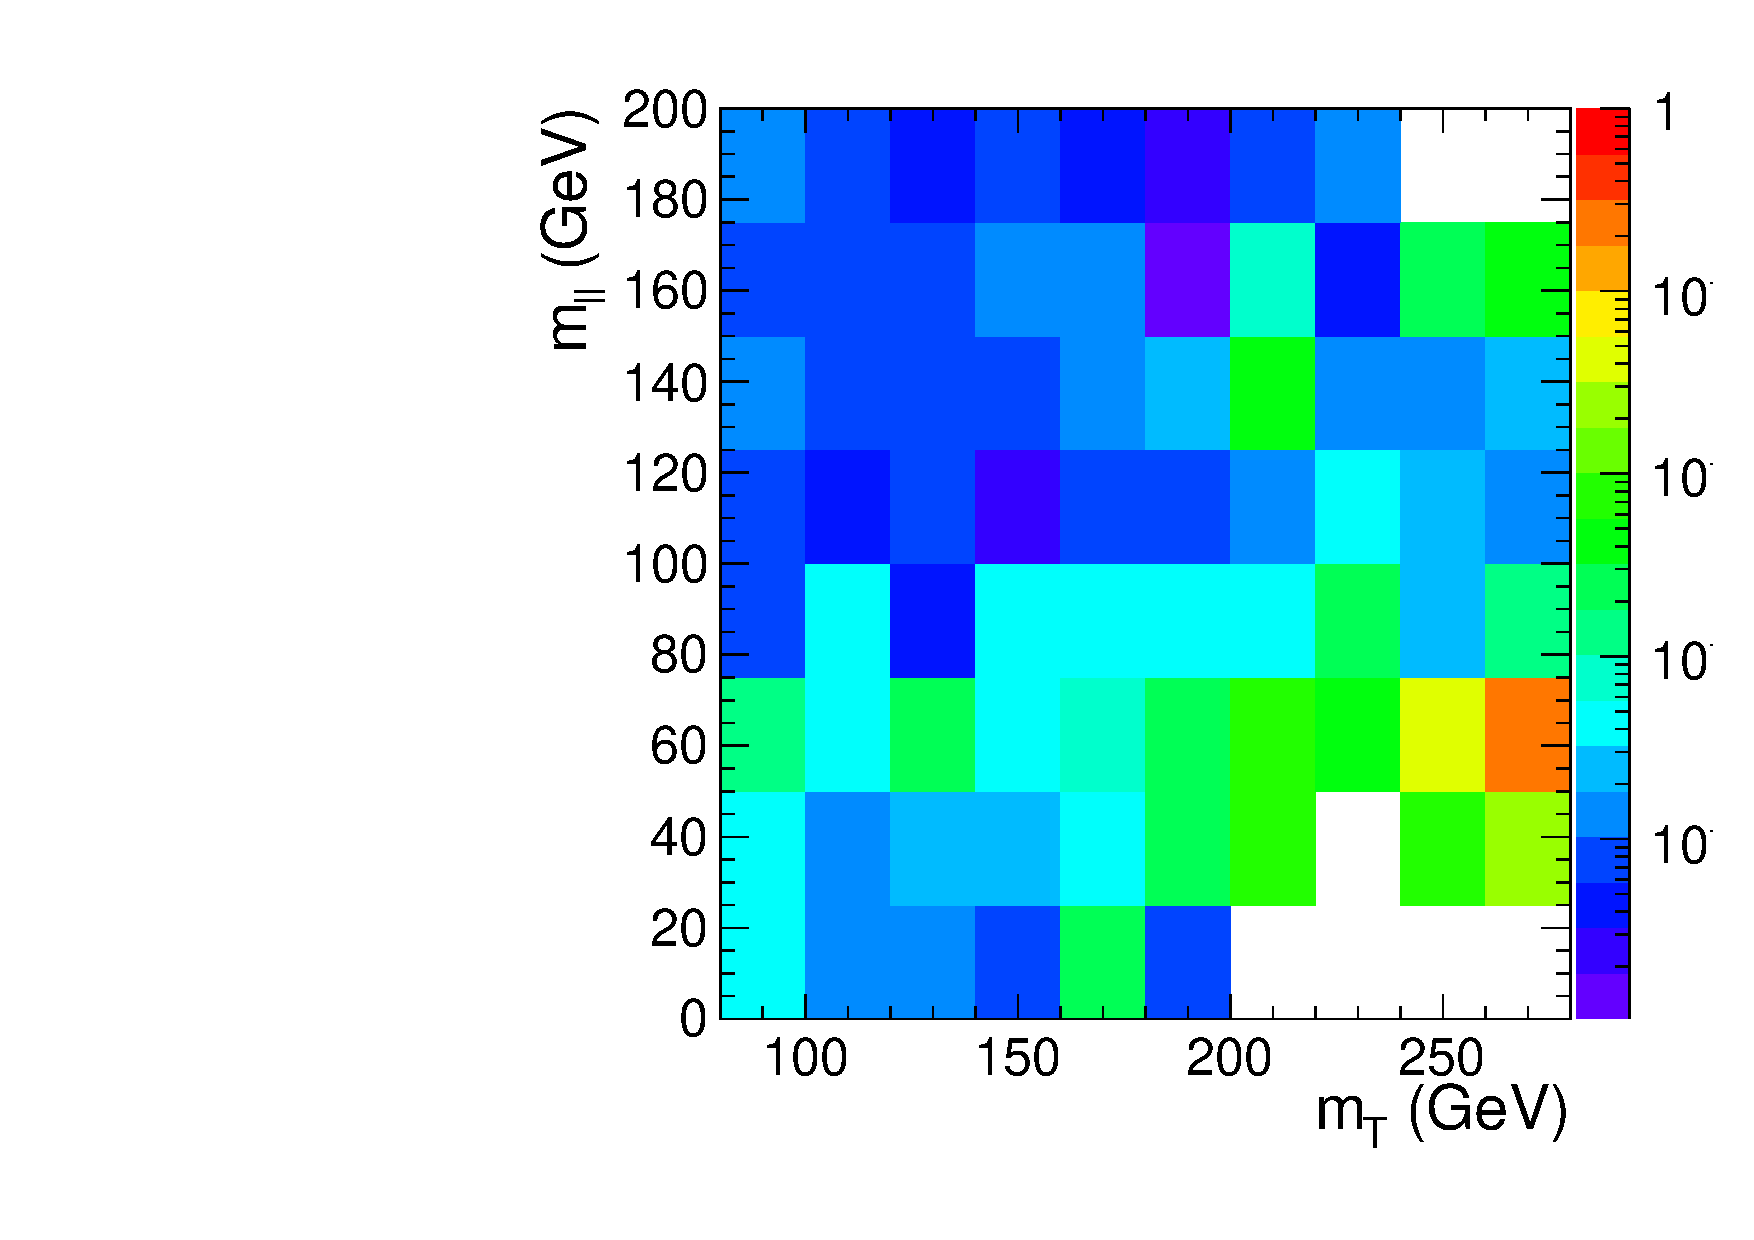
\includegraphics[width=.35\textwidth]{figures/templates/Zjetserr_2D_mH160_0j_of.pdf}
	}

	%
	\centering
	\subfigure[Wgamma]{
	\centering
	\label{subfig:template_Wgamma_160}
		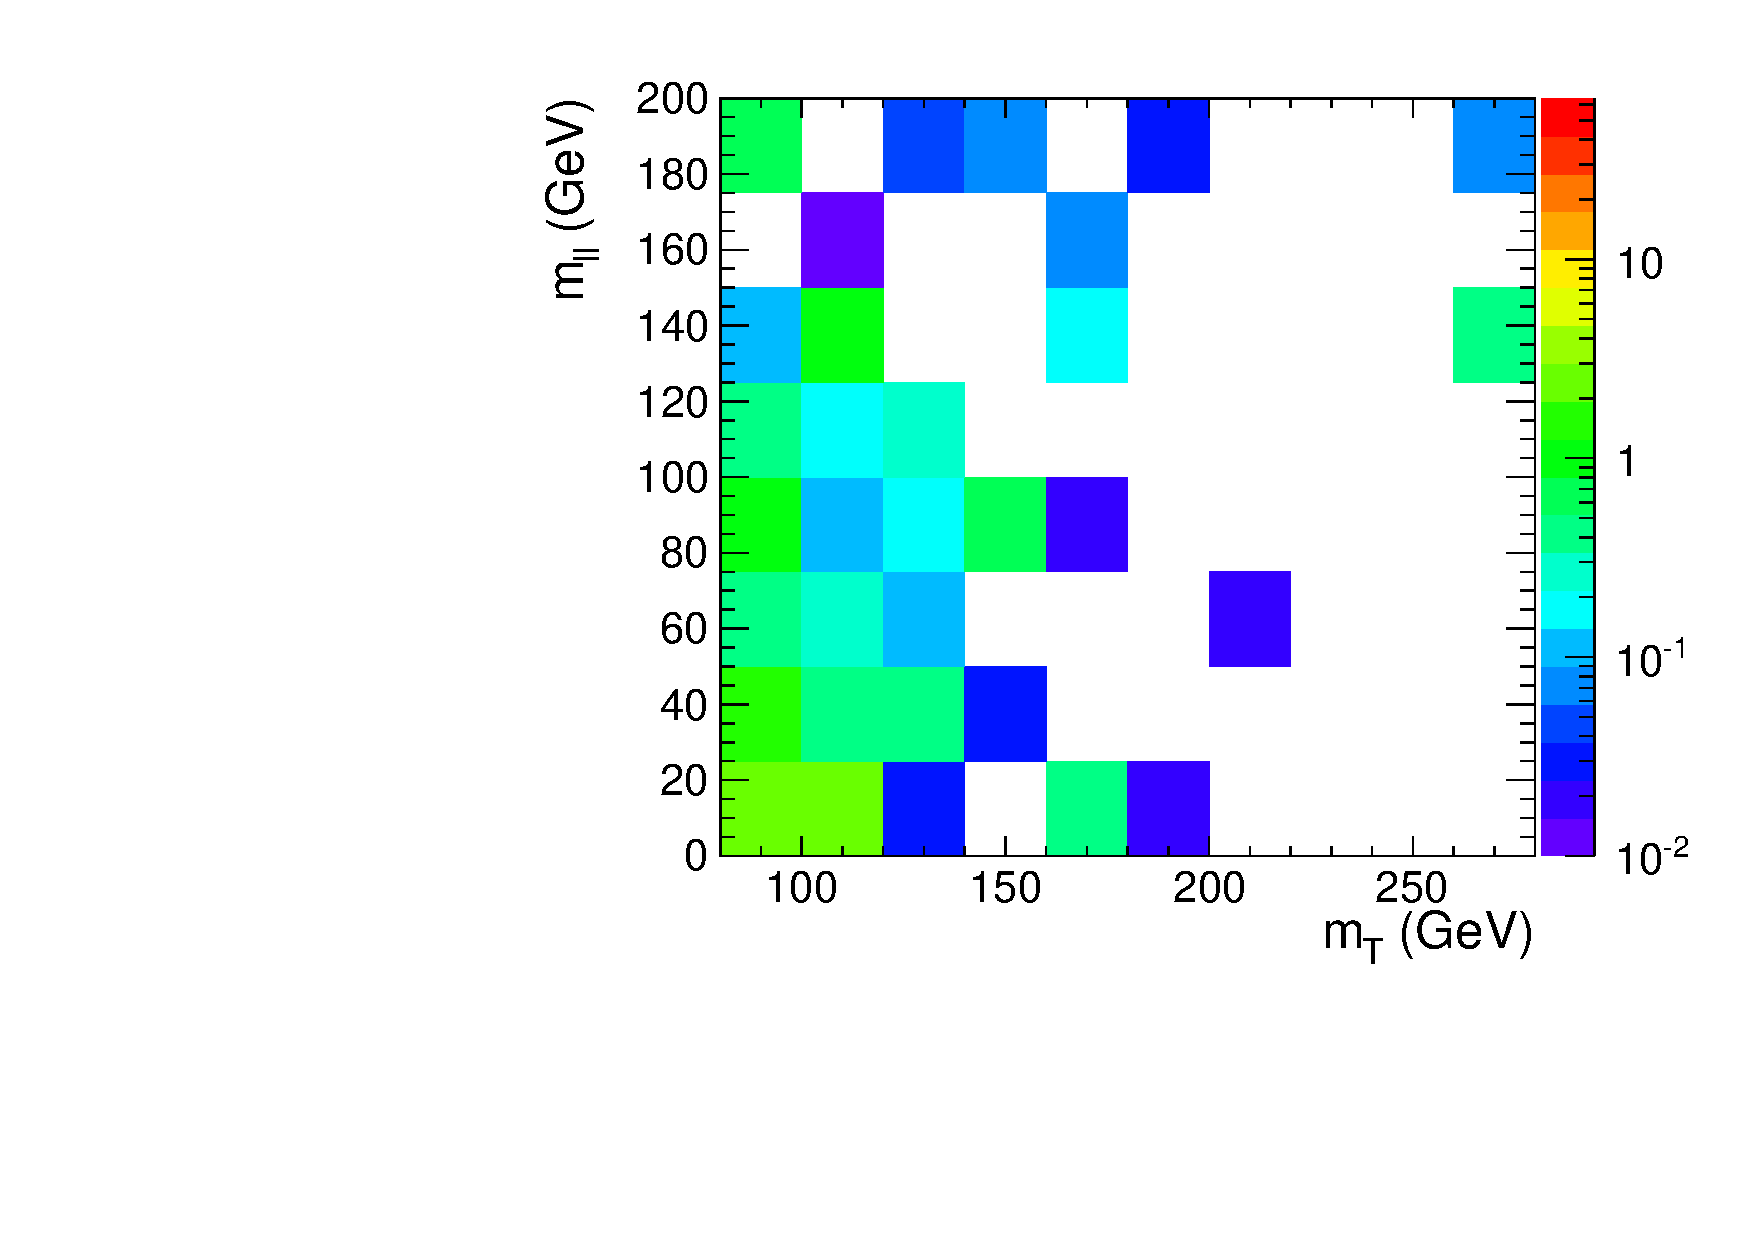
\includegraphics[width=.35\textwidth]{figures/templates/Wgamma_2D_mH160_0j_of.pdf}
	}
	\subfigure[Wgamma statistical uncertainty]{
	\centering
	\label{subfig:template_Wgammaerr_160}
		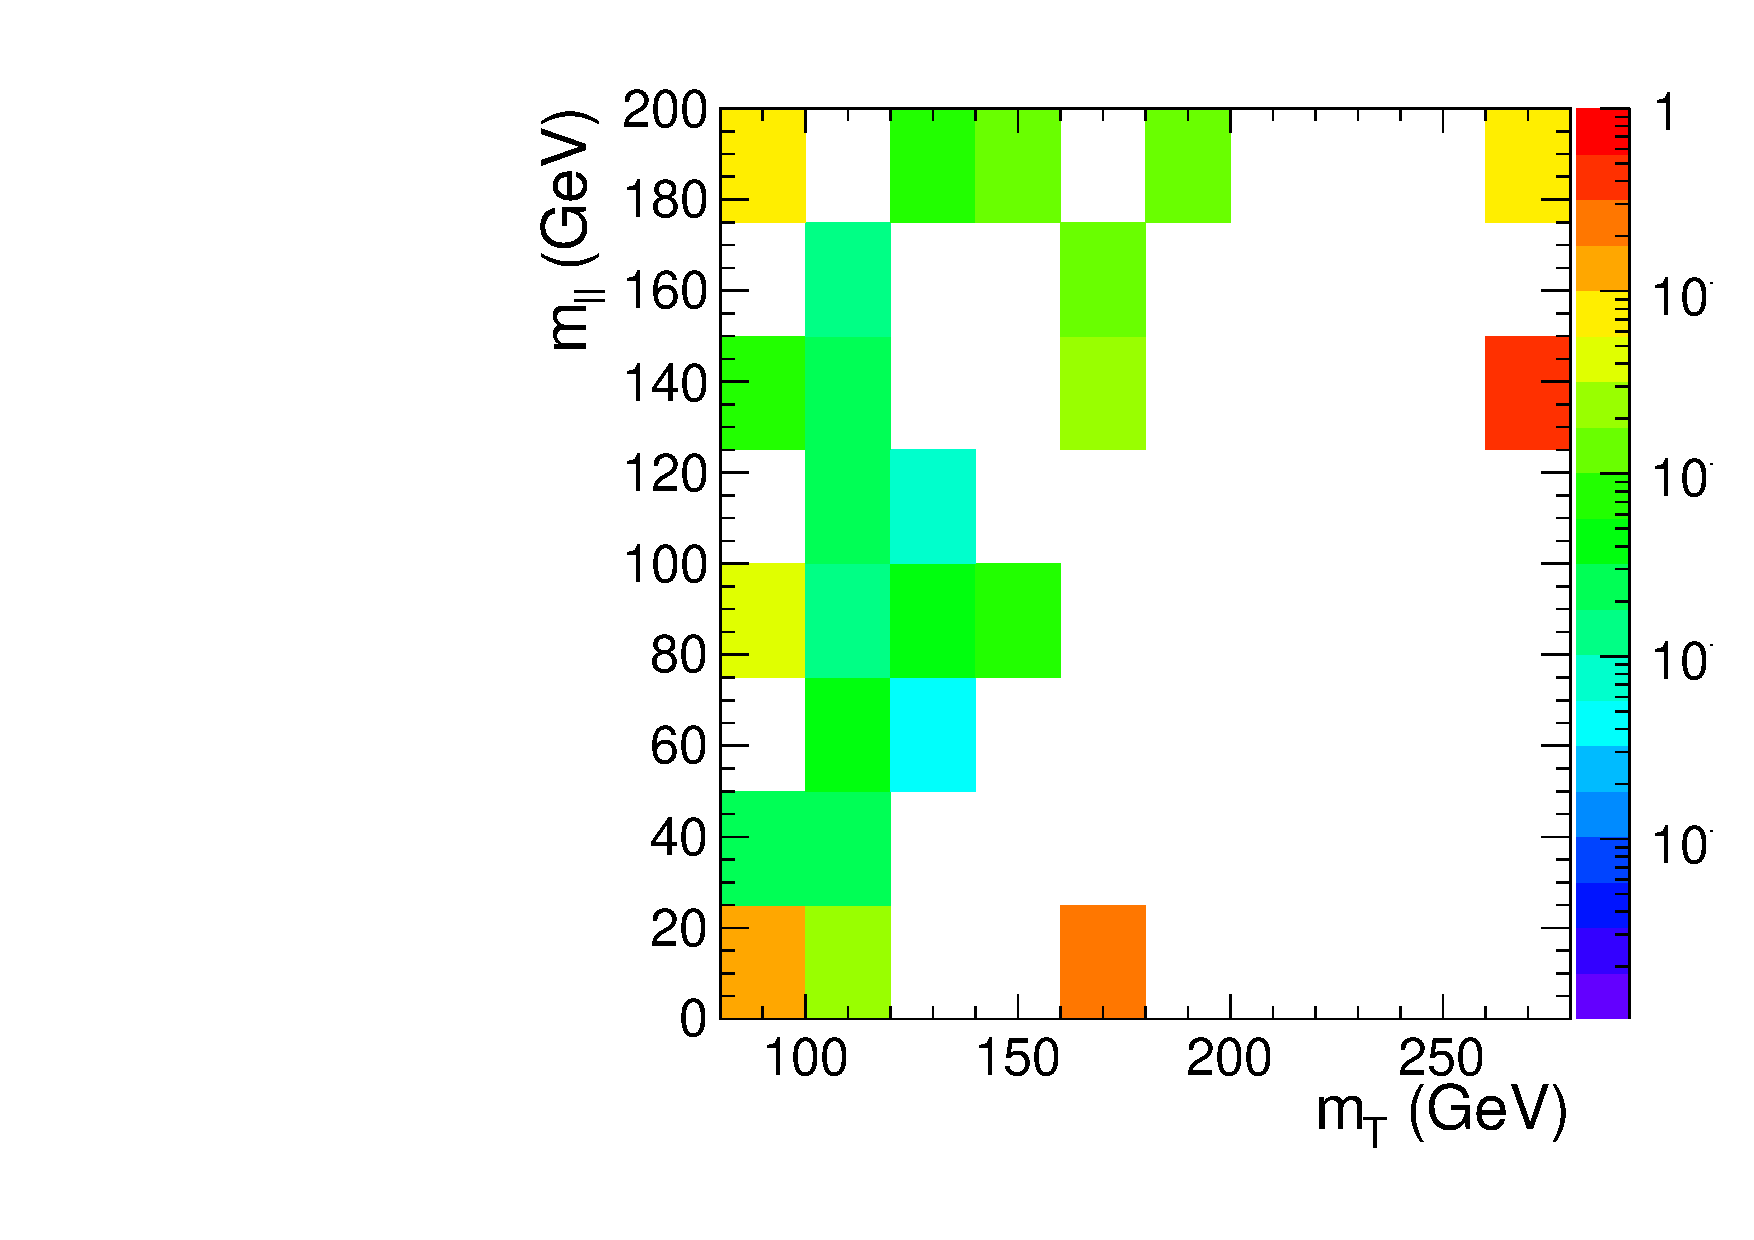
\includegraphics[width=.35\textwidth]{figures/templates/Wgammaerr_2D_mH160_0j_of.pdf}
	}

	\caption{2D templates at \mHi = 160 \GeV} 
	\label{fig:templates_160_3}

\end{figure} 

\begin{figure}[!hbtp]
	
	%
	\centering
	\subfigure[Stacked unrolled template linear]{
	\centering
	\label{subfig:template_unroll_stack_lin}
		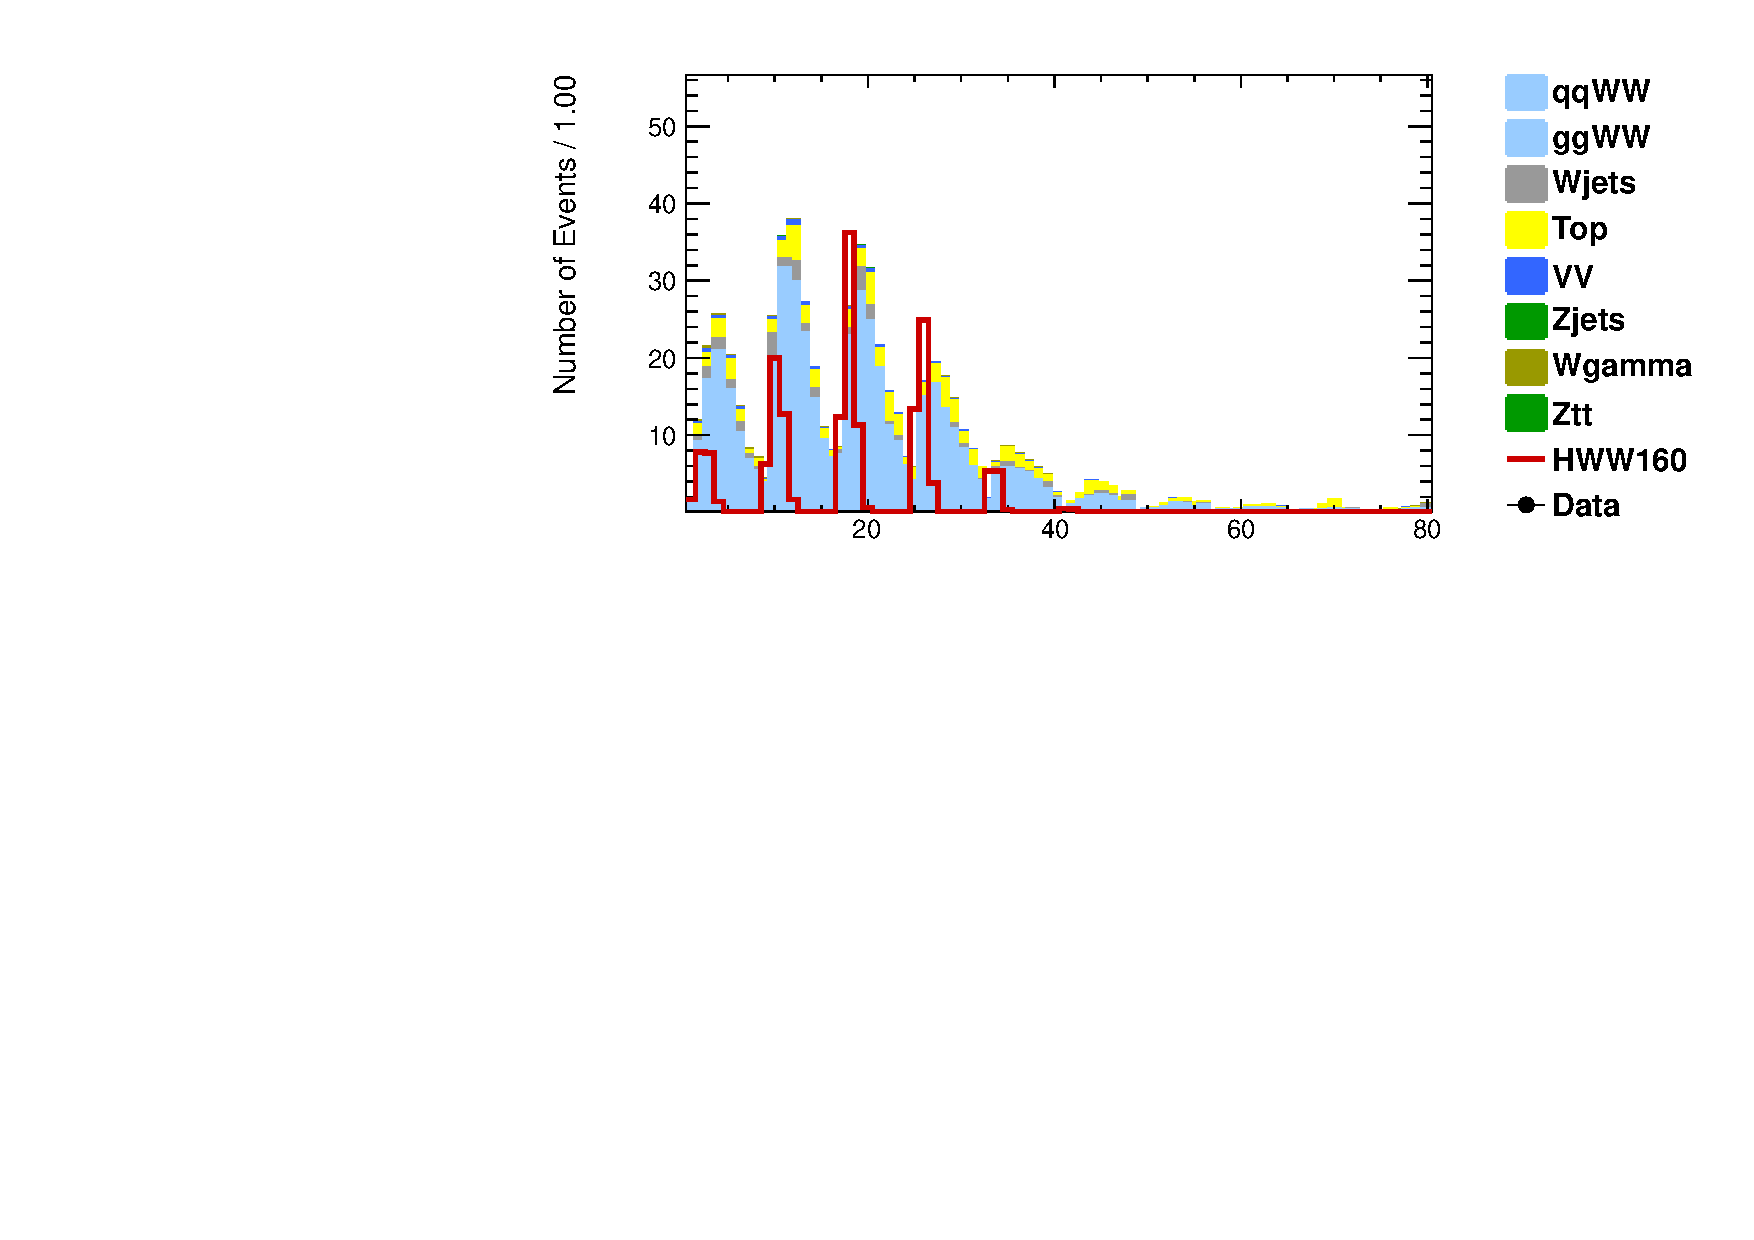
\includegraphics[width=.45\textwidth]{figures/templates/2D_mH160_0j_of_stack_lin.pdf}
	}
	\subfigure[Overlaid unrolled template linear]{
	\centering
	\label{subfig:template_unroll_overlay_lin}
		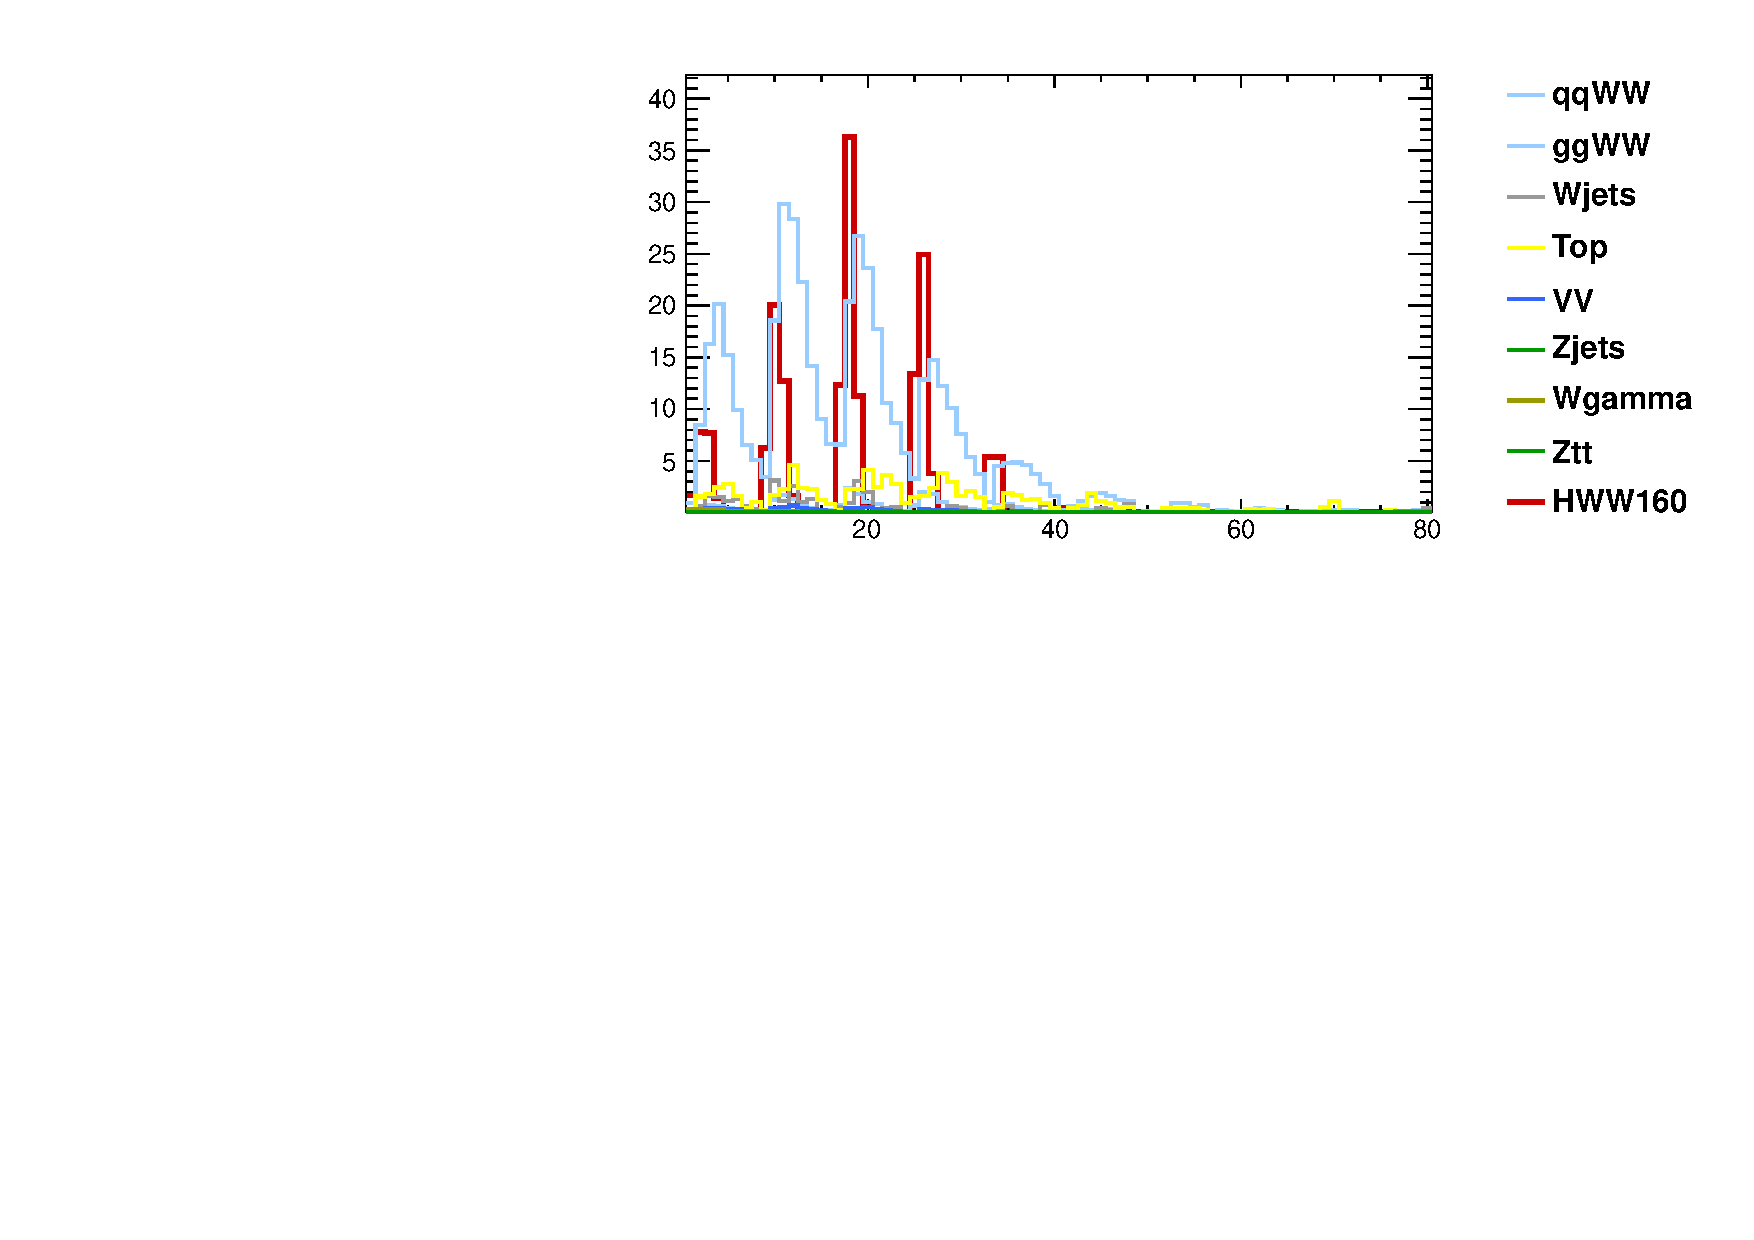
\includegraphics[width=.45\textwidth]{figures/templates/2D_mH160_0j_of_overlay_lin.pdf}
	}

	%
	\centering
	\subfigure[Stacked unrolled template in log scale]{
	\centering
	\label{subfig:template_unroll_stack_log}
		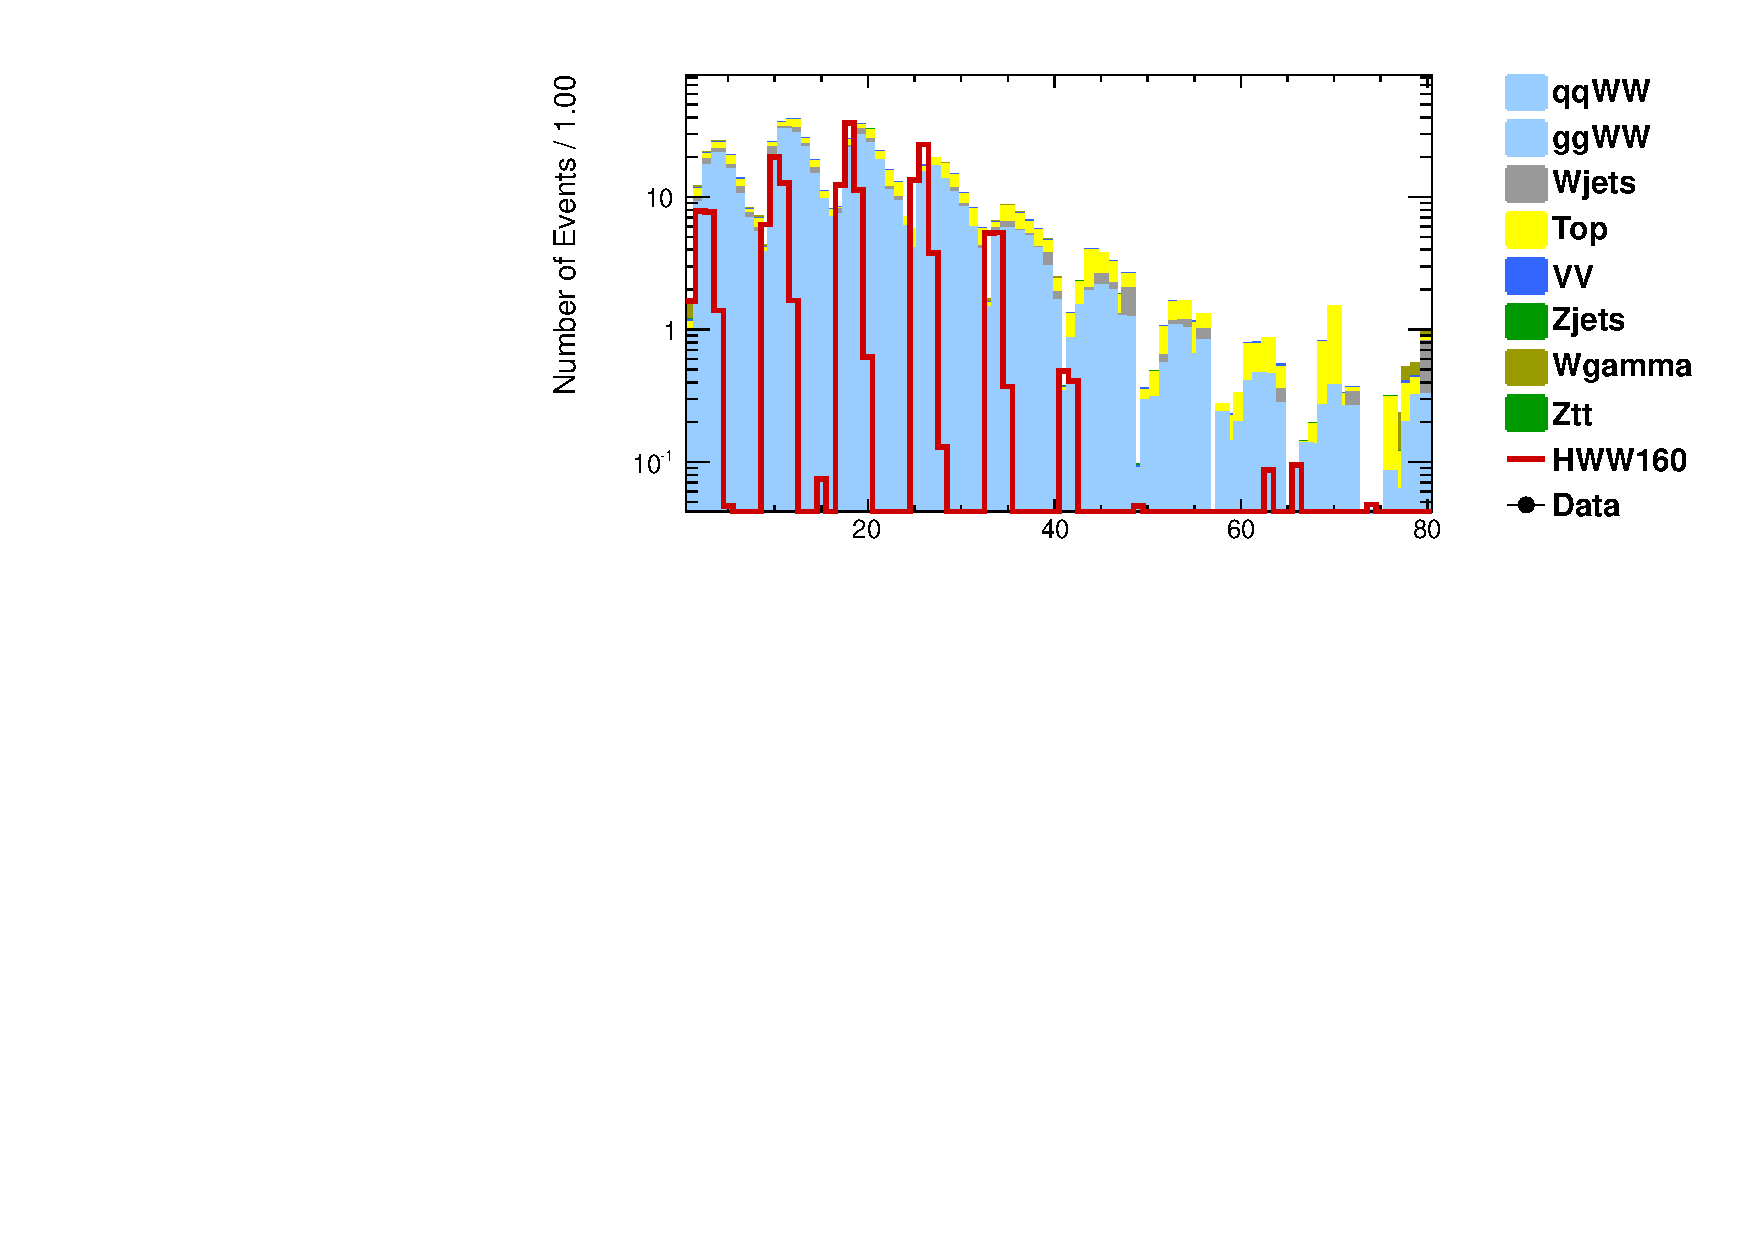
\includegraphics[width=.45\textwidth]{figures/templates/2D_mH160_0j_of_stack_log.pdf}
	}
	\subfigure[Overlaid unrolled template in log scale]{
	\centering
	\label{subfig:template_unroll_overlay_log}
		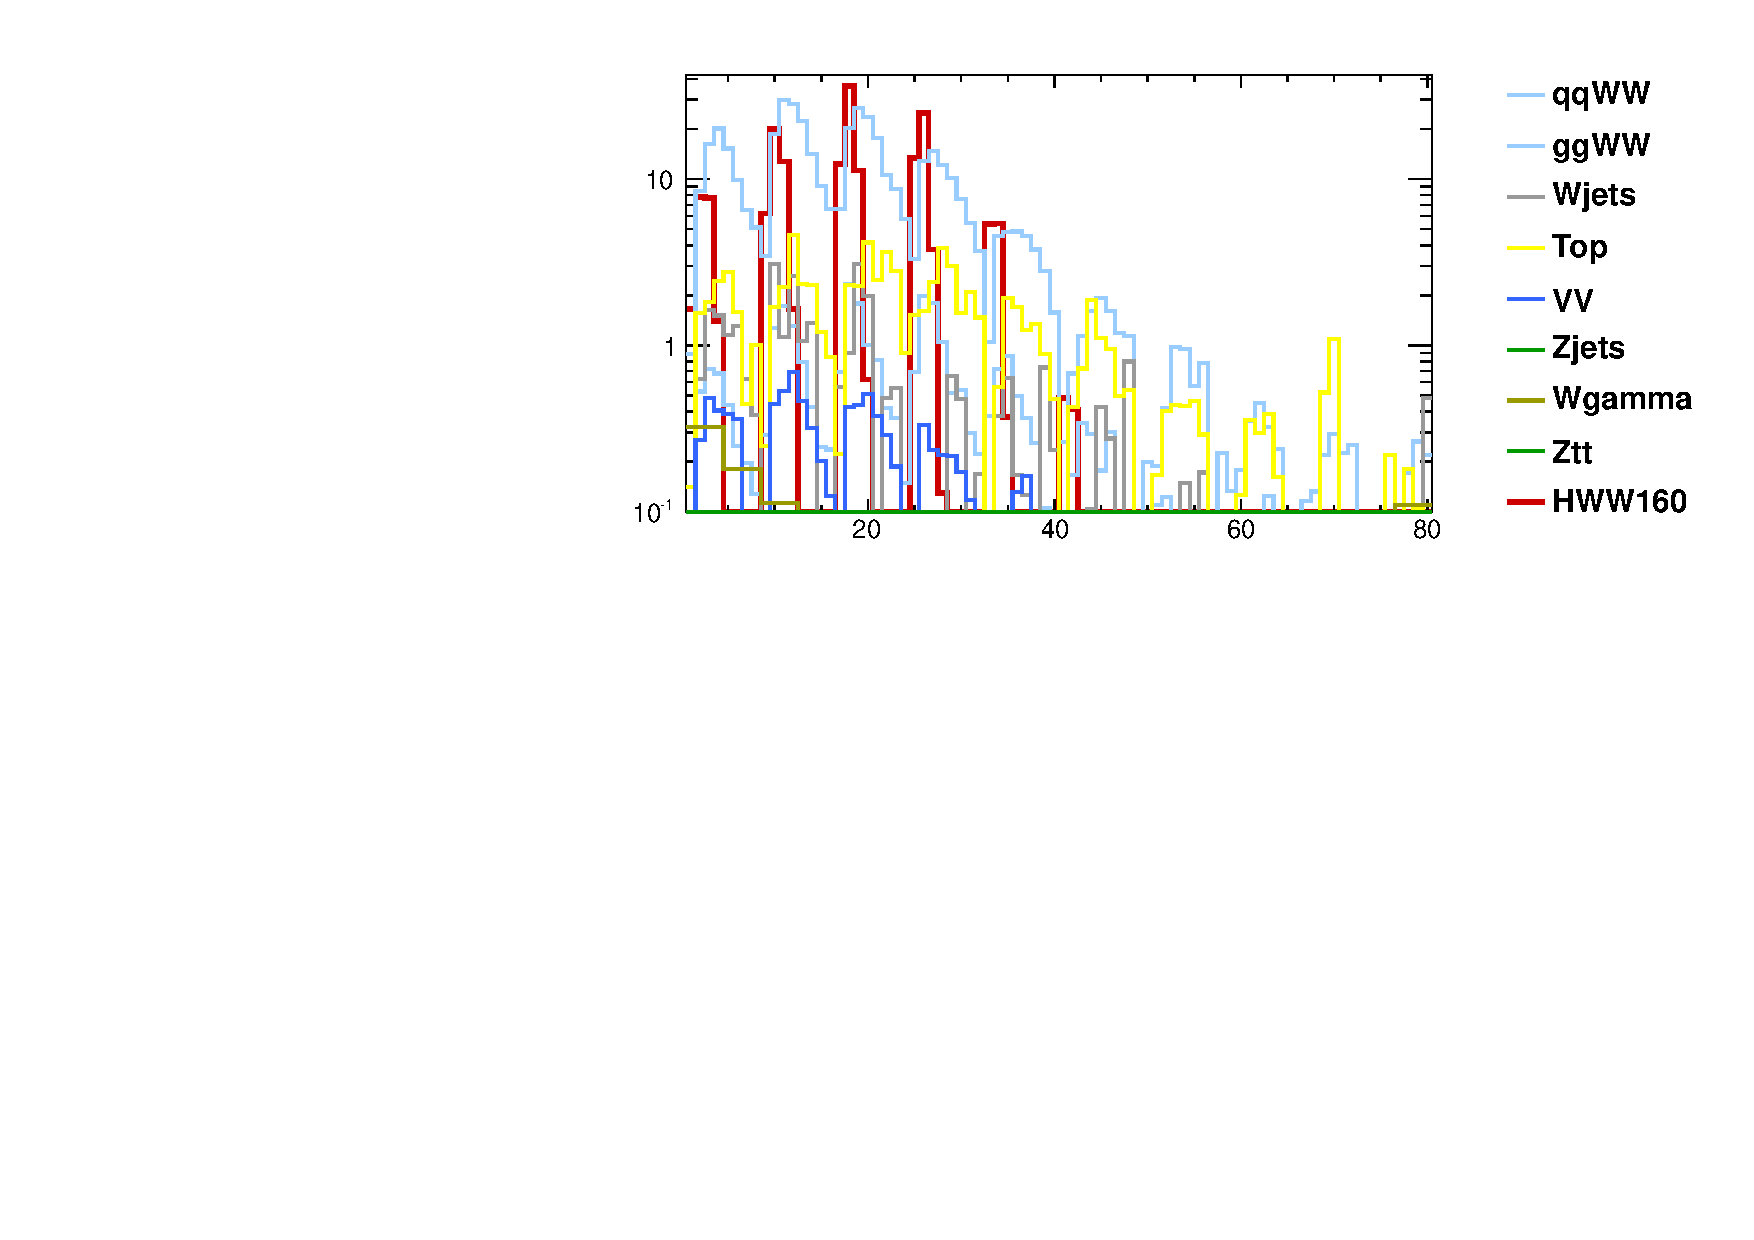
\includegraphics[width=.45\textwidth]{figures/templates/2D_mH160_0j_of_overlay_log.pdf}
	}

	\caption{Unrolled templates at \mHi = 160 \GeV} 
	\label{fig:templates_160_unroll}

\end{figure} 

%%%%%% mH=200 GeV
\begin{figure}[!hbtp]
	
	%
	\centering
	\subfigure[Signal]{
	\centering
	\label{subfig:template_signal_200}
		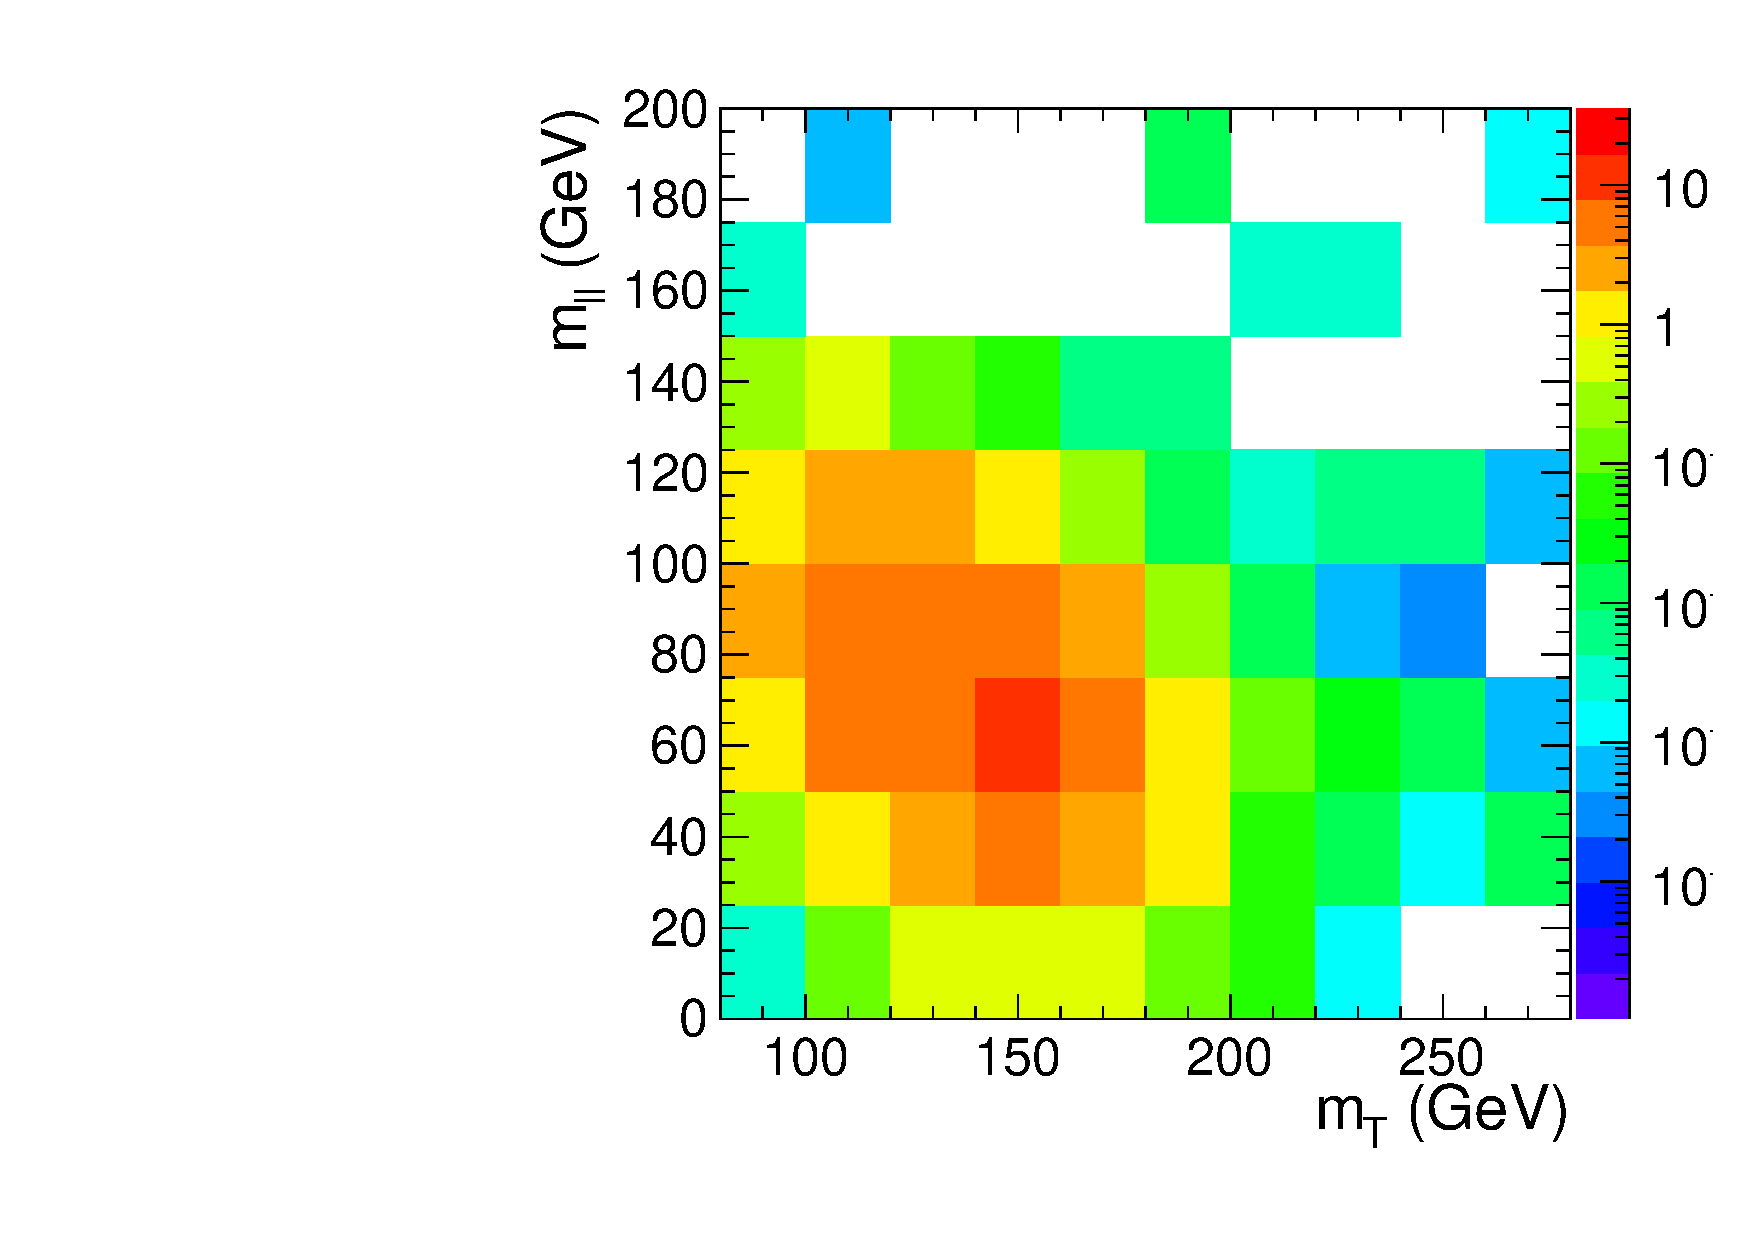
\includegraphics[width=.35\textwidth]{figures/templates/sig_2D_mH200_0j_of.pdf}
	}
	\subfigure[Signal statistical uncertainty]{
	\centering
	\label{subfig:template_signalerr_200}
		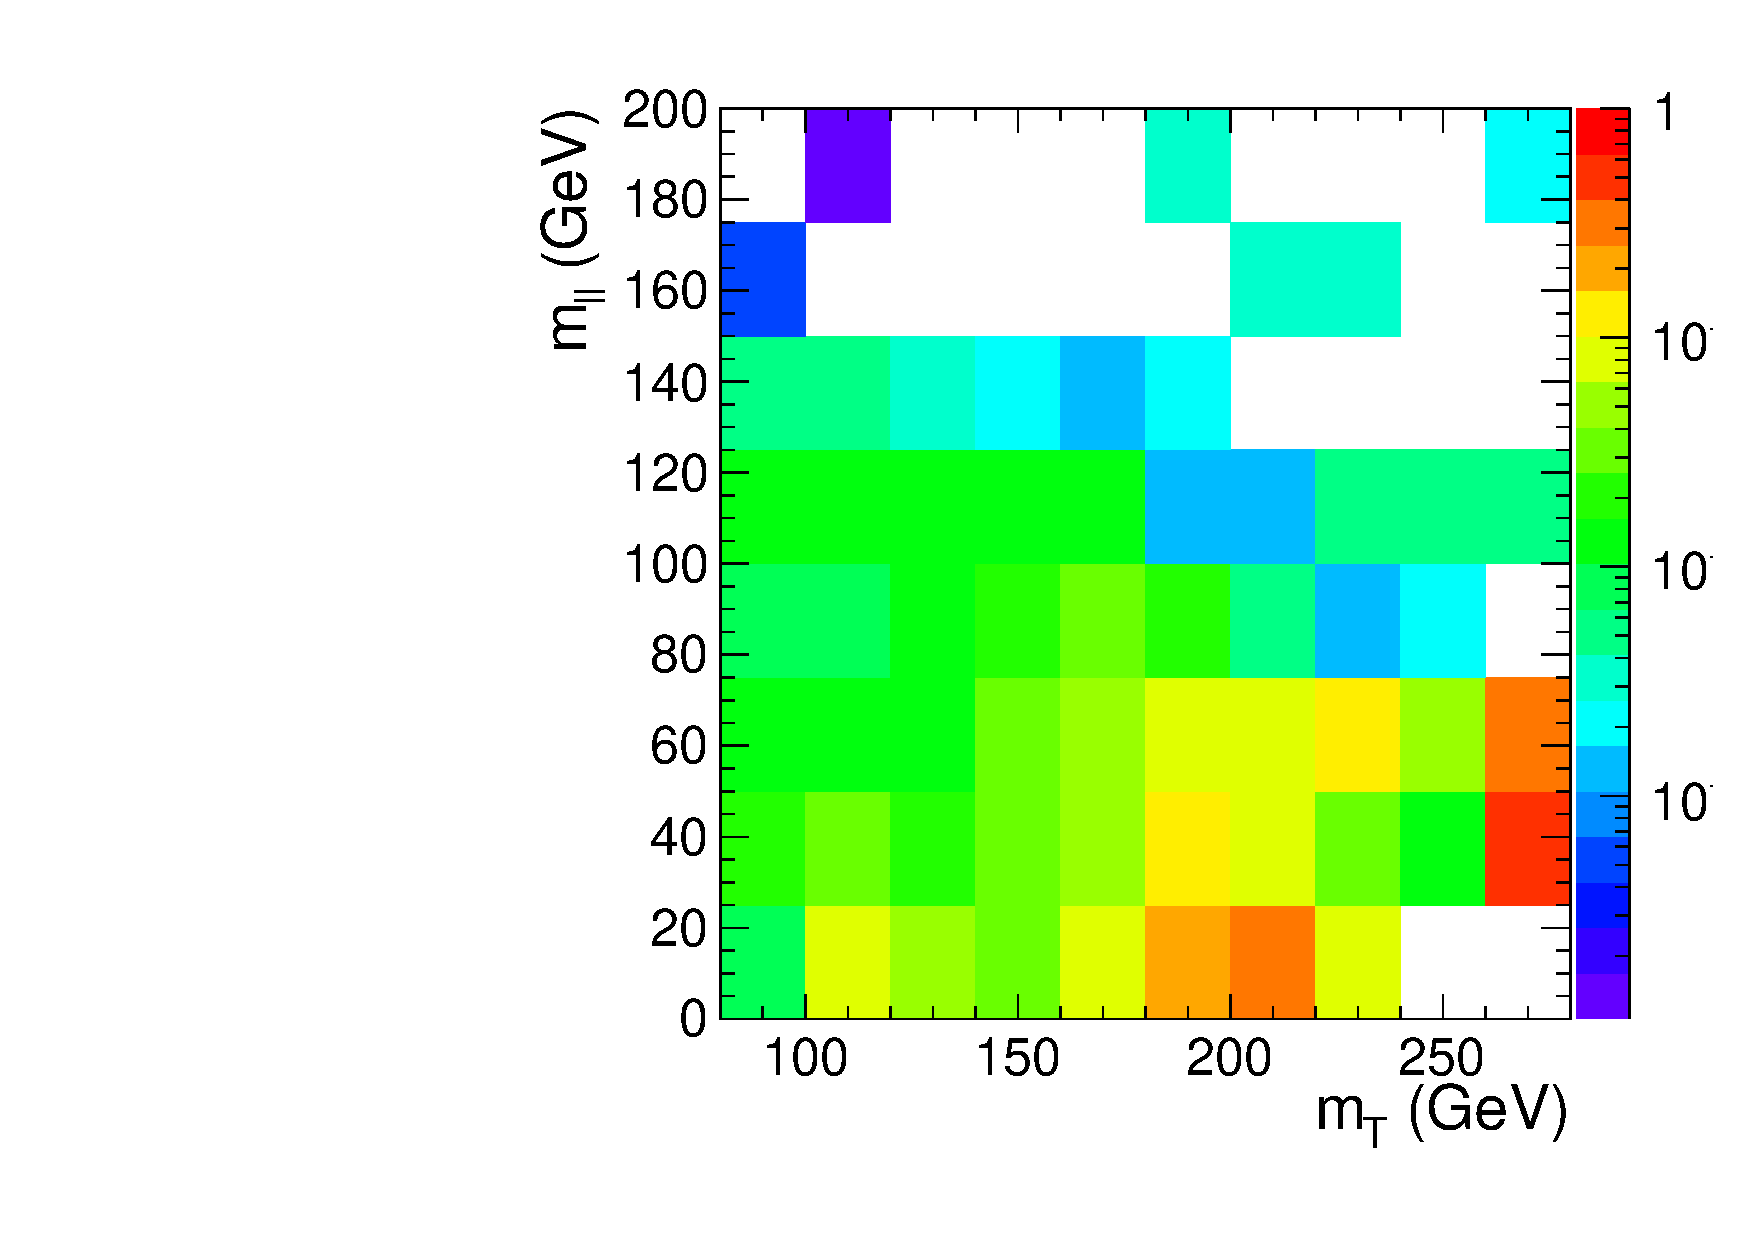
\includegraphics[width=.35\textwidth]{figures/templates/sigerr_2D_mH200_0j_of.pdf}
	}
	
	%
	\centering
	\subfigure[qqWW]{
	\centering
	\label{subfig:template_qqWW_200}
		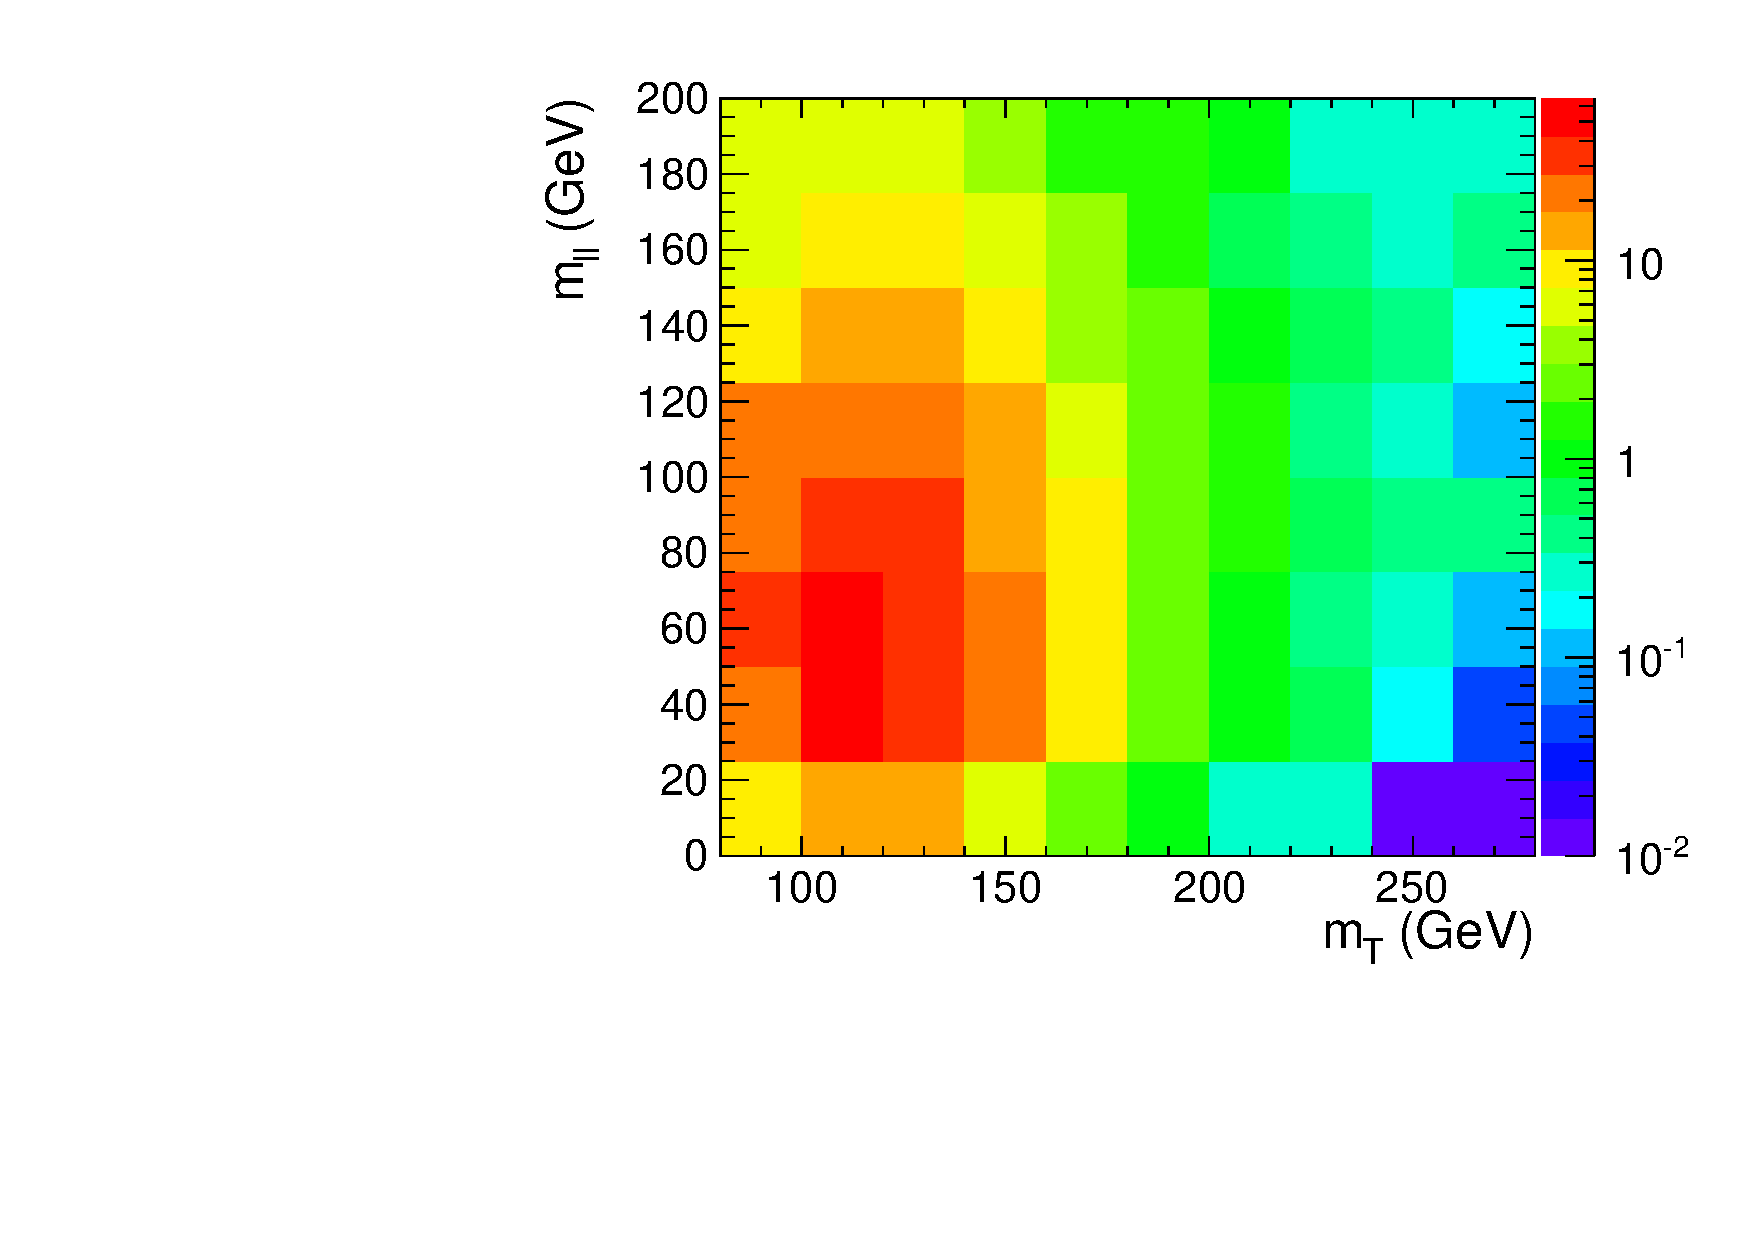
\includegraphics[width=.35\textwidth]{figures/templates/qqWW_2D_mH200_0j_of.pdf}
	}
	\subfigure[qqWW statistical uncertainty]{
	\centering
	\label{subfig:template_qqWWerr_200}
		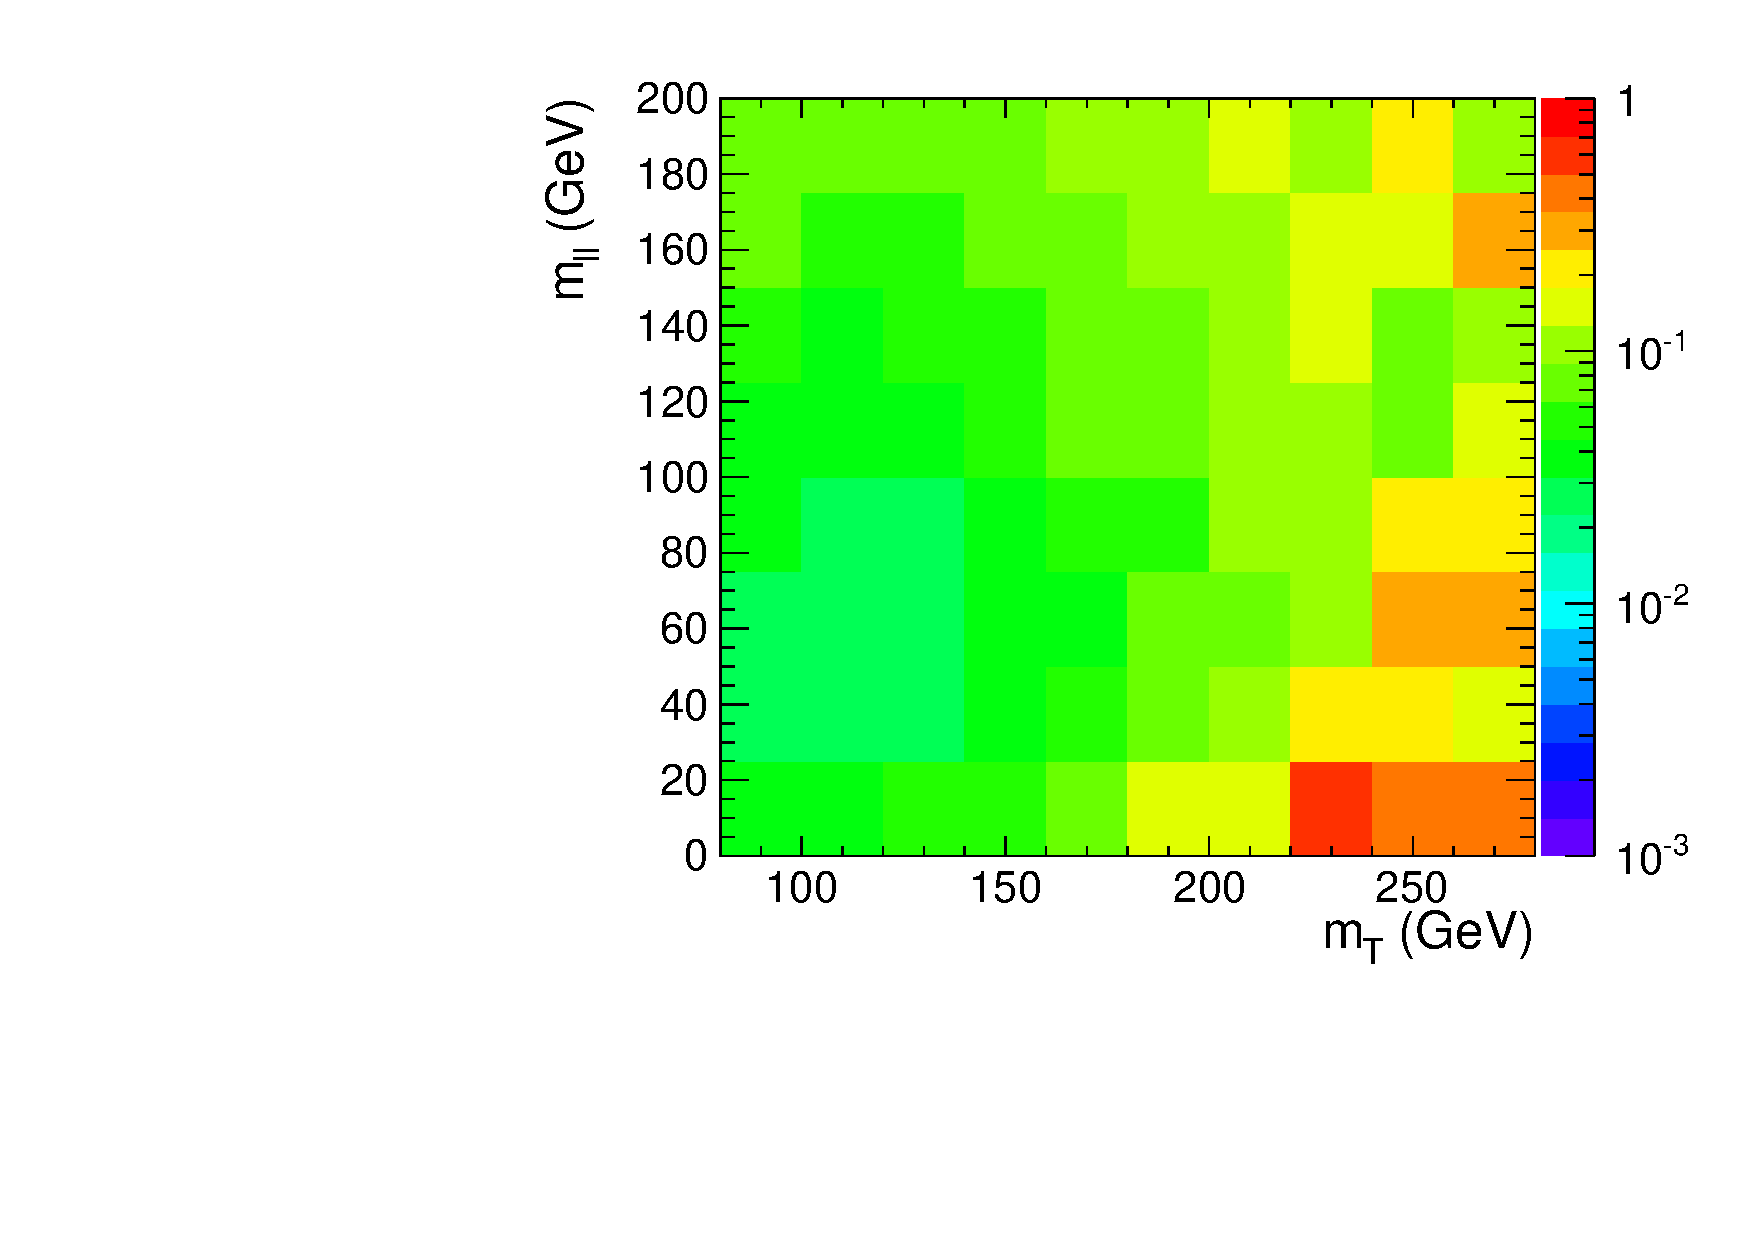
\includegraphics[width=.35\textwidth]{figures/templates/qqWWerr_2D_mH200_0j_of.pdf}
	}

	%
	\centering
	\subfigure[ggWW]{
	\centering
	\label{subfig:template_ggWW_200}
		\includegraphics[width=.35\textwidth]{figures/templates/ggWW_2D_mH200_0j_of.pdf}
	}
	\subfigure[ggWW statistical uncertainty]{
	\centering
	\label{subfig:template_ggWWerr_200}
		\includegraphics[width=.35\textwidth]{figures/templates/ggWWerr_2D_mH200_0j_of.pdf}
	}

	\caption{2D templates at \mHi = 200 \GeV} 
	\label{fig:templates_200_1}

\end{figure}

\begin{figure}[!hbtp]
	
	%
	\centering
	\subfigure[Wjets]{
	\centering
	\label{subfig:template_Wjets_200}
		\includegraphics[width=.35\textwidth]{figures/templates/Wjets_2D_mH200_0j_of.pdf}
	}
	\subfigure[Wjets statistical uncertainty]{
	\centering
	\label{subfig:template_Wjetserr_200}
		\includegraphics[width=.35\textwidth]{figures/templates/Wjetserr_2D_mH200_0j_of.pdf}
	}
	
	%
	\centering
	\subfigure[Top]{
	\centering
	\label{subfig:template_Top_200}
		\includegraphics[width=.35\textwidth]{figures/templates/Top_2D_mH200_0j_of.pdf}
	}
	\subfigure[Top statistical uncertainty]{
	\centering
	\label{subfig:template_Toperr_200}
		\includegraphics[width=.35\textwidth]{figures/templates/Toperr_2D_mH200_0j_of.pdf}
	}

	%
	\centering
	\subfigure[VV]{
	\centering
	\label{subfig:template_VV_200}
		\includegraphics[width=.35\textwidth]{figures/templates/VV_2D_mH200_0j_of.pdf}
	}
	\subfigure[VV statistical uncertainty]{
	\centering
	\label{subfig:template_VVerr_200}
		\includegraphics[width=.35\textwidth]{figures/templates/VVerr_2D_mH200_0j_of.pdf}
	}

	\caption{2D templates at \mHi = 200 \GeV} 
	\label{fig:templates_200_2}

\end{figure}

\begin{figure}[!hbtp]
	
	%
	\centering
	\subfigure[Zjets]{
	\centering
	\label{subfig:template_Zjets_200}
		\includegraphics[width=.35\textwidth]{figures/templates/Zjets_2D_mH200_0j_of.pdf}
	}
	\subfigure[Zjets statistical uncertainty]{
	\centering
	\label{subfig:template_Zjetserr_200}
		\includegraphics[width=.35\textwidth]{figures/templates/Zjetserr_2D_mH200_0j_of.pdf}
	}

	%
	\centering
	\subfigure[Wgamma]{
	\centering
	\label{subfig:template_Wgamma_200}
		\includegraphics[width=.35\textwidth]{figures/templates/Wgamma_2D_mH200_0j_of.pdf}
	}
	\subfigure[Wgamma statistical uncertainty]{
	\centering
	\label{subfig:template_Wgammaerr_200}
		\includegraphics[width=.35\textwidth]{figures/templates/Wgammaerr_2D_mH200_0j_of.pdf}
	}

	\caption{2D templates at \mHi = 200 \GeV} 
	\label{fig:templates_200_3}

\end{figure} 

\begin{figure}[!hbtp]
	
	%
	\centering
	\subfigure[Stacked unrolled template linear]{
	\centering
	\label{subfig:template_unroll_stack_lin}
		\includegraphics[width=.45\textwidth]{figures/templates/2D_mH200_0j_of_stack_lin.pdf}
	}
	\subfigure[Overlaid unrolled template linear]{
	\centering
	\label{subfig:template_unroll_overlay_lin}
		\includegraphics[width=.45\textwidth]{figures/templates/2D_mH200_0j_of_overlay_lin.pdf}
	}

	%
	\centering
	\subfigure[Stacked unrolled template in log scale]{
	\centering
	\label{subfig:template_unroll_stack_log}
		\includegraphics[width=.45\textwidth]{figures/templates/2D_mH200_0j_of_stack_log.pdf}
	}
	\subfigure[Overlaid unrolled template in log scale]{
	\centering
	\label{subfig:template_unroll_overlay_log}
		\includegraphics[width=.45\textwidth]{figures/templates/2D_mH200_0j_of_overlay_log.pdf}
	}

	\caption{Unrolled templates at \mHi = 200 \GeV} 
	\label{fig:templates_200_unroll}

\end{figure} 

  
  \newpage
  \section{S/B with various bin sizes}
     \label{app:binsize}
     \begin{figure}[htp]
	\centering
	\includegraphics[width=1.0\textwidth]{figures/binsize.pdf}
	\caption{ blah }
  	\label{fig:app_binsize}
\end{figure}

Figure~\ref{fig:app_binsize} shows S/B in the unrolled templates. 
Bins with large signal contribution are shown with different bin sizes. 
S/B does not change much by the size of bins.  
Thus, we choose the largest bin size of the choices to get maximum statistics in each bin.  


\end{document}
